% 使用 XeLaTeX 编译。封面必须保留，学校、队号及姓名仅出现在封面。
\documentclass[bwprint]{gmcmthesis}

% === 额外宏包（cls 未内置的）===
\usepackage[framemethod=TikZ]{mdframed}
\usepackage[section]{placeins}
\usepackage{needspace}
\usepackage{subfig}
\usepackage{float}
\usepackage{algorithm2e}

% === TikZ ===
\usepackage{tikz}
\usetikzlibrary{arrows.meta,positioning,shapes.geometric,fit,calc}
\usepackage{longtable}
\usepackage{booktabs}
\usepackage{multirow}

% === 引用上标格式 ===
\setcitestyle{super,square,comma}

% === 竞赛信息 ===
\title{山区洪涝灾害下无人机运输与通信协同优化\\ ——基于等效航程能耗模型与中继布设的联合调度设计}
\baominghao{[参赛队号]}
\schoolname{[学校名称]}
\membera{[成员A]}
\memberb{[成员B]}
\memberc{[成员C]}

\begin{document}

\maketitle

% === 摘要 ===
\begin{abstract}

本文针对广西横州市镇龙乡山区洪涝灾害场景下的应急物资无人机运输与全程通信
保障问题，按单点组批、异构机队调度、运输与中继联合调度、任务分区与资源配置
四个层次递进建立优化模型，并以数字高程模型、无人机与电池参数和通信链路参数
逐问求解、逐级校验。全部计算基于 Python 实现，飞行时间、能耗与通信链路均按
题给统一规则建模，任一结果均可由随附脚本复算。

\textbf{问题一：单点往返最大安全载荷与货箱组批。}以等效航程法把水平飞行能耗
折算为可用电量乘以航程与等效航程之比，叠加爬升能耗与返航安全裕度
百分之二十的约束，对三机型与十五服务区组成的四十五个组合逐一二分求最大安全载荷。
结果中 A 型全部取质量上限 25\,kg，B 型取 30\,kg（仅 S008 受能量约束降为
约 28.9\,kg），C 型多数取 80\,kg，而 S002、S003、S004、S008、S012 五个远区
受能量约束，分别为 69.0、68.4、63.9、59.2、68.2\,kg。按机型与服务区组批共
18 架次，总能耗 59.02\,kWh，累计作业时间约 9.1\,h，各架次返航荷电状态均不低于
百分之二十。安全余量扫描表明，余量比例由 0.2 升到 0.35 时架次由 18 增至 25，
能耗由 59.02 升至 77.63\,kWh，增幅约 31.5\%，安全与效率存在明确权衡。

\textbf{问题二：异构无人机多点多架次调度。}以架次为决策单元，按时限贪心组批
生成初始解并拆出紧急架次，再并行比较模拟退火、遗传算法、自适应大邻域搜索、
禁忌搜索与 GRASP，并以多权重--多种子强化搜索收敛 Pareto 前沿。调度层按截止期
优先，并耦合无人机与电池双资源就绪队列求可行派单；评估按严格口径执行，\textbf{
每个货箱的投递时刻所属服务区必须与其箱号归属区一致}（区一致零违例），凡
"捎带"结算者一律判不可行。选取零迟到的禁忌搜索均衡方案：
25 架次，其中 A 型 11、B 型 8、C 型 6，完工时间约 118.5\,min（7113\,s），
总能耗 70.28\,kWh，全部 80 箱按各自时限、投送至各自指定服务区交付，加权迟到
为零。相较原遗传算法均衡方案，完工提前约 20.5\,min（14.7\%）、能耗降低约
7.0\,kWh（9.1\%）；若以能耗为先，可选用 21 架次方案
（约 131\,min、62.46\,kWh）。

\textbf{问题三：通信约束下运输与中继联合调度。}建立频率 2400\,MHz 的自由空间
传播加地形遮挡的电波模型，接收门限为负 90\,dBm，直连、接入、回程链路上限为
122、116、126\,dB，并按 30\,m 步长沿航线逐点判定遮挡。覆盖采样确定三个中继
布设点，W 点服务西与北片区，E 点服务东片区，N 点服务 S004；对 25 架次区一致
方案沿航线审核得到 1394 个需中继采样点，初始布设即实现全覆盖、运输无需平移。
以该方案为运输层输入，两架中继按时间分片复用：W 点单班，服务时段
716 至 6777\,s（能耗 2.082\,kWh）；E 点服务时段 760 至 3354\,s，
能耗 0.986\,kWh；N 点服务时段 3409 至 4135\,s，能耗 0.483\,kWh，
中继合计约 3.55\,kWh，回程链路全部可行，各班能耗均低于单架次能源上限。
联合完工由运输最后返场 7113\,s（约 118.5\,min）决定，中继约束引入的完工
代价为零，全部 80 箱仍按各自时限投送至指定服务区交付、加权迟到为零，
覆盖盲区为零。

\textbf{问题四：任务分区与资源配置。}按中继覆盖结构给出
三组与两组两种分区（25 架次中多区架次均落在同一覆盖片区内，无跨片区同组
约束），对每组以最小机队搜索
确定机型与电池数量，再叠加冗余备份核算库存。结果表明，若按组完全独立配置，
两种分区均超出库存，例如两组方案需 A 型机 6 架超出 2 架、B 型机 5 架超出
3 架、C 型机 3 架超出 1 架、中继 5 架超出 3 架；分三组时重复配置更多。给定库存下
更优组织为任务分区、资源池化，即分区仅用于任务组织，机队与中继仍集中调度并
时间分片复用，问题三的协同方案以 8 架运输机、14 组电池、2 架中继恰好满足库存，
实现零迟到与零盲区；若坚持独立配置，需增配 A 型机 2 架、B 型机 3 架、
C 型机 1 至 3 架、A 型电池 2 至 3 组、B 型电池 3 组、C 型电池 0 至 2 组、
中继 3 至 5 架与能源组件 1 至 3 组。

\textbf{灵敏度分析}表明模型结论稳健：安全余量扫描复现安全效率权衡并呈现机型
结构切换；多目标权重在合理范围内只改变拆分粒度，不改变 C 型瓶颈结构；中继
W 点最长连续服务 101\,min，占单架次能源上限对应时长约 140\,min 的 72.2\%，
悬停功率扰动正负百分之十后方案不变；通信余量统计中 W 点最紧 1.00\,dB、E 点
1.10\,dB、N 点 9.40\,dB，三个布设点均无低于 1\,dB 的采样点，余量下压 1\,dB
仅个别采样点接近门限，布设方案整体对链路参数不敏感。

\keywords{无人机调度\quad 等效航程能耗模型\quad 禁忌搜索\quad 中继布设\quad 任务分区\quad 通信保障}
\end{abstract}

\pagestyle{plain}

% === 正文 ===
% 问题重述
\section{问题重述}
\label{sec:background}

\subsection{问题背景}

2026 年 7 月，广西横州市镇龙乡遭受严重洪涝灾害，道路与桥梁损毁，多处村屯
成为与外界隔绝的孤岛\cite{refXinhua,refXinhua2}。应急物资只能依赖无人机从
调度中心 O01 空运至各受灾服务区。镇龙乡属典型山区地形，山峰与沟谷高差达数百
米，低空飞行易被山体遮挡，无人机与调度中心之间的无线电通信难以全程保持视距
链路，成为应急投送的关键瓶颈。图 \ref{fig:map} 给出研究区域内的数字高程模型
与调度节点分布，可见 O01 与 S001 至 S015 共 15 个服务区散布于河谷与山脊之间。

\begin{figure}[htbp]
\centering
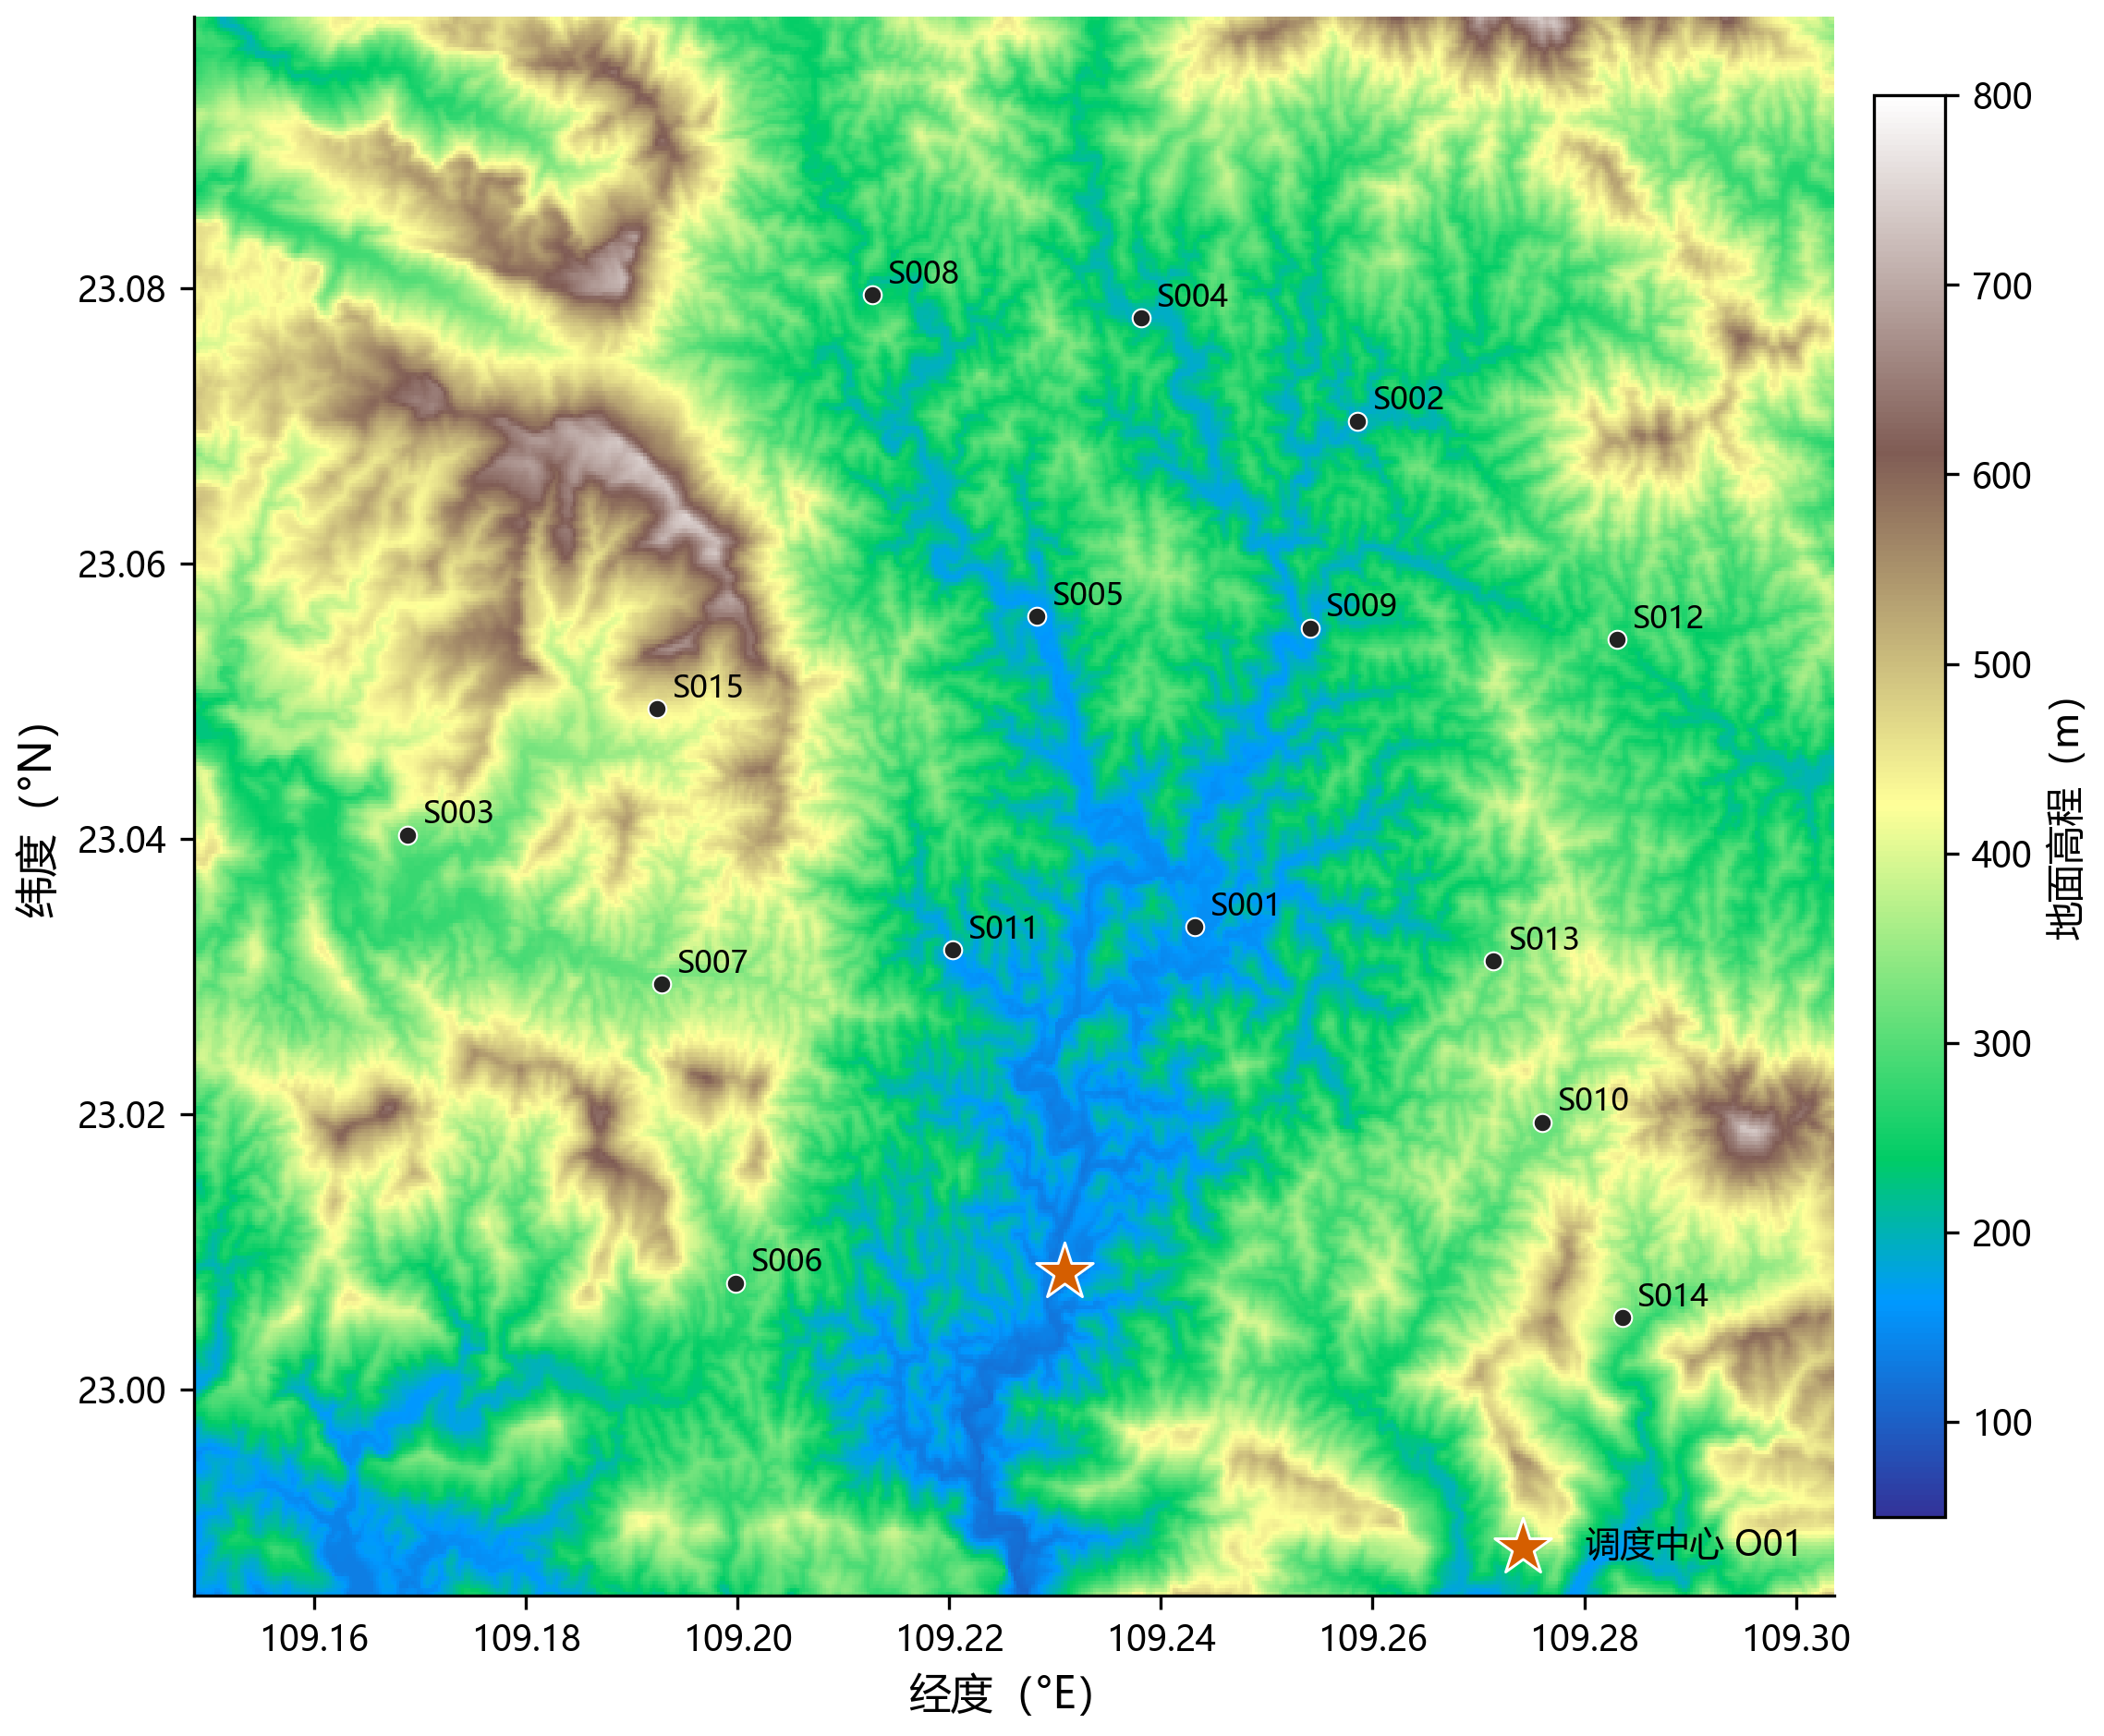
\includegraphics[width=0.78\textwidth]{figures/p1_map.png}
\caption{研究区域数字高程模型与调度节点分布（O01 为调度中心，圆点为服务区）}
\label{fig:map}
\end{figure}

本问题给出 O01 与 15 个服务区的经纬度与地面高程、30\,m 分辨率的数字高程模型、
三类运输无人机与配套电池、两架中继无人机与能源组件，以及 80 个待投运货箱
（分医疗物资、饮用水、应急食品、生活卫生用品四类，各有质量、体积与配送时限）。
题目要求在山区约束下设计无人机运输方案，并保证无人机全程通信不中断。

\subsection{问题提出}

本问题要求依次求解以下四个子问题。

\textbf{问题一：单点往返最大安全载荷与货箱组批。}针对每类运输无人机到各服务
区的单点往返任务，考虑飞行时间、载荷能耗与返航安全余量，确定单架次最大安全
载荷，并据此把各服务区货箱合理分组，给出每类机型的组批方案与架次能耗、返航
荷电状态。

\textbf{问题二：异构无人机多点多架次调度。}15 个服务区的 80 个货箱具有不同配送
时限，机队由 A、B、C 三类共 8 架无人机与 14 组共享电池组成，即 A 型 6 组、B 型 4 组、C 型 4 组。要求合理安排
各架次的任务序列、起降时刻与电池分配，使全部货箱按时送达，并尽量少用架次、
降低总能耗与总完工时间。

\textbf{问题三：通信约束下运输与中继联合调度。}无人机整个飞行过程必须与调度
中心保持通信，通信可采用直连或经悬停中继的双跳方式。中继无人机的最佳布设
位置与架次安排需结合山区地形与电波传播模型确定，并与运输调度联合优化，实现全程
无盲区且运输效率不劣化。

\textbf{问题四：任务分区与资源配置。}将 15 个服务区划分为两组与三组两种方案，
按组配备运输无人机、电池、中继无人机及能源组件等资源，考虑冗余备份，说明各
组能否独立完成保障任务，并给出资源配置方案。
% 模型假设
\section{模型假设}
\label{sec:assume}

为使问题可解并保证模型与题目规则一致，作如下假设。

\begin{enumerate}
\item \textbf{飞行运动学假设}：无人机垂直起飞与降落，爬升与下降速度恒为
$v_{\mathrm{up}}$ 与 $v_{\mathrm{down}}$；水平巡航按航线匀速飞行，速度为
$v_c$。航线巡航高度取航段上各点地面高程的最大值再加 50\,m 安全余量，即
$h_{\mathrm{cruise}}=\max_{x\in leg}\mathrm{DEM}(x)+50$\,m；服务区内作业高度
取该区地面高程，按悬停 30\,s 投递计入时延。飞行时间按三段相加，即
$t=h^+/v_{\mathrm{up}}+d/v_c+h^-/v_{\mathrm{down}}$。

\item \textbf{载荷能耗假设}：水平飞行单位里程能耗由等效航程函数 $L_g(q)$
刻画，该函数随载荷 $q$ 增大而缩短；水平能耗等于可用电量乘以航程与等效航程
之比，即 $E_{\mathrm{hor}}=E_{\mathrm{use}}\cdot d/L_g(q)$。爬升段为克服重力
做功，即 $E_{\mathrm{up}}=(m_0+q)gh^+/(\eta\cdot3.6\times10^6)$\,kWh，下降段
近似忽略。任意架次总能耗不得超过返航安全上限，即
$E_{\mathrm{total}}\le(1-\rho)E_{\mathrm{use}}$，其中 $\rho=20\%$ 为返航安全
余量。

\item \textbf{电池与充电假设}：每个架次出发前在 O01 更换满电电池；返航后电池
按两阶段曲线充电，即荷电状态低于 0.9 时充电时长为
$T\cdot(0.65\cdot(0.9-SOC)/0.9+0.35)$，否则为
$T\cdot0.35\cdot(1-SOC)/0.1$；充电完成的电池才可再次出勤，同一块电池同一时刻
仅供一架无人机使用。

\item \textbf{通信传播假设}：信号按自由空间传播衰减，附加系统损耗
$L_{\mathrm{sys}}=3$\,dB 与地形遮挡损耗 $L_{\mathrm{obs}}=10$\,dB；接收灵敏度
$P_{\mathrm{sens}}=-98$\,dBm，解调余量 $M=8$\,dB，即接收门限
$P_{\mathrm{th}}=-90$\,dBm。判定通信有效需链路总损耗不超过直连、接入、回程
三档上限（122、116、126\,dB）之一，且收发两端间不存在地形遮挡，即在连线
上以 30\,m 步长采样，任一点地形高于连线则判遮挡。

\item \textbf{中继假设}：中继无人机由 O01 起飞，悬停于候选位置执行转发任务，
悬停高度按与地面链路衔接要求取布设点高程以上一定高度且不超过 300\,m；每次
任务含 180\,s 起飞准备、30\,s 建链、服务时段与转场时间；中继单架次能源预算为
$(1-\rho)E_{\mathrm{use}}=2.56$\,kWh，超出则须返场充电再出勤。

\item \textbf{资源约束假设}：每架无人机任一时刻只能执行一个任务；货箱不可
分包，即一个货箱由单一架次一次送达；暂不考虑气象、禁飞区与无人机故障，
故障冗余问题见第\ref{sec:p4}节。
\end{enumerate}
% 符号说明
\section{符号说明}
\label{sec:symbol}

主要符号及其含义如表 \ref{tab:symbols} 所示，其余符号在文中首次出现处说明。

\begin{table}[htbp]
\centering
\caption{主要符号说明}
\label{tab:symbols}
\begin{tabular}{clcl}
\toprule
符号 & 含义 & 符号 & 含义 \\
\midrule
$O01$ & 调度中心 & $S_i$ & 第 $i$ 个服务区（$i=1,\dots,15$）\\
$q$ & 架次载荷（kg） & $Q_m$ & 机型 $m$ 最大载荷 \\
$m_0$ & 无人机空机质量 & $g$ & 重力加速度 \\
$v_c,\,v_{\mathrm{up}},\,v_{\mathrm{down}}$ & 巡航/爬升/下降速度 & $d$ & 水平航线距离 \\
$h^+,\,h^-$ & 爬升/下降高度 & $\eta$ & 电机效率 \\
$E_{\mathrm{use}}$ & 满载标称可用电量 & $E_{\mathrm{hor}},\,E_{\mathrm{up}}$ & 水平/爬升能耗 \\
$L_g(q)$ & 载荷 $q$ 下等效航程 & $L_0,\,L_F$ & 空载/满载等效航程 \\
$\rho$ & 返航安全裕度（$20\%$） & $SOC$ & 电池荷电状态 \\
$T$ & 电池满充时长 & $d_1,\,d_e$ & 首飞批/普通批时限 \\
$f$ & 工作频率（$2400$\,MHz） & $L_{\mathrm{FSPL}}$ & 自由空间损耗 \\
$L_{\mathrm{sys}},\,L_{\mathrm{obs}}$ & 系统/遮挡损耗 & $P_{\mathrm{sens}},\,P_{\mathrm{th}}$ & 接收灵敏度/门限 \\
$M$ & 解调余量 & $D$ & 收发间三维距离 \\
$t_{\mathrm{link}},\,t_{\mathrm{prep}}$ & 建链/准备时间 & $P_W,P_E,P_N$ & 三个中继布设点 \\
\bottomrule
\end{tabular}
\end{table}
% 问题一
\section{问题一：单点往返最大安全载荷与货箱组批}
\label{sec:p1}

\subsection{问题分析}

问题一包含两层任务，其一是对每类运输无人机到各服务区的单点往返任务，在满足
飞行时间、载荷能耗与返航安全余量约束下求最大安全载荷；其二是依据该载荷及各
服务区货箱的质量、体积与时限，把货箱分组为架次，使总架次数与总能耗最小。
核心在于建立可核验的载荷、能耗、返航荷电状态映射：载荷越大，等效航程越短、
单位里程能耗越高，架次能耗随之上升，因此最大安全载荷由质量上限、体积上限与
能量上限三者中的最紧者决定。

\subsection{模型建立}

\subsubsection{飞行时间模型}

对航线 O01 到服务区再到 O01 的往返，设航段水平距离 $d$（按大圆距离计算），
航线最高地面高程与起飞点地面高程之差为 $h^+$，返回段下降高度为 $h^-$，
单架次飞行时间按式 \eqref{eq:time} 计算。

\begin{equation}
t_{\mathrm{fly}}= \frac{h^+}{v_{\mathrm{up}}} + \frac{d}{v_c}
+ \frac{h^-}{v_{\mathrm{down}}}
\label{eq:time}
\end{equation}

其中巡航高度为 $h_{\mathrm{cruise}}=\max_{x\in leg}\mathrm{DEM}(x)+50$\,m，
作业高度取服务区地面高程，投递悬停 30\,s。

\subsubsection{能耗模型}

按题目统一规则，水平飞行能耗由等效航程函数折算，等效航程按式
\eqref{eq:lg} 计算。

\begin{equation}
L_g(q) = L_0 - (L_0 - L_F)\left(\frac{q}{Q}\right)^{1.5}
\label{eq:lg}
\end{equation}

水平能耗为 $E_{\mathrm{hor}} = E_{\mathrm{use}}\cdot d/L_g(q)$；爬升段能耗按式
\eqref{eq:eup} 计算。

\begin{equation}
E_{\mathrm{up}} = \frac{(m_0+q)\,g\,h^+}{\eta\cdot 3.6\times10^6}\ \mathrm{kWh}
\label{eq:eup}
\end{equation}

单架次总能耗为水平能耗与爬升能耗之和，返航安全约束按式 \eqref{eq:cap}
给出，其中安全余量 $\rho=20\%$。

\begin{equation}
E_{\mathrm{total}} \le (1-\rho)\,E_{\mathrm{use}},\qquad \rho=20\%
\label{eq:cap}
\end{equation}

同时受载荷与货舱体积约束，即 $q\le Q_m$、$\sum V \le V_{\max}$。

图 \ref{fig:lgcurve} 左图给出三类机型的等效航程随载荷收缩的曲线，右图给出
三机型到 S008 往返的能耗随载荷变化，水平虚线为各自的返航安全上限，交点即
能量约束下的最大安全载荷，可见 C 型因满载航程收缩最快而最先触及上限。

\begin{figure}[htbp]
\centering
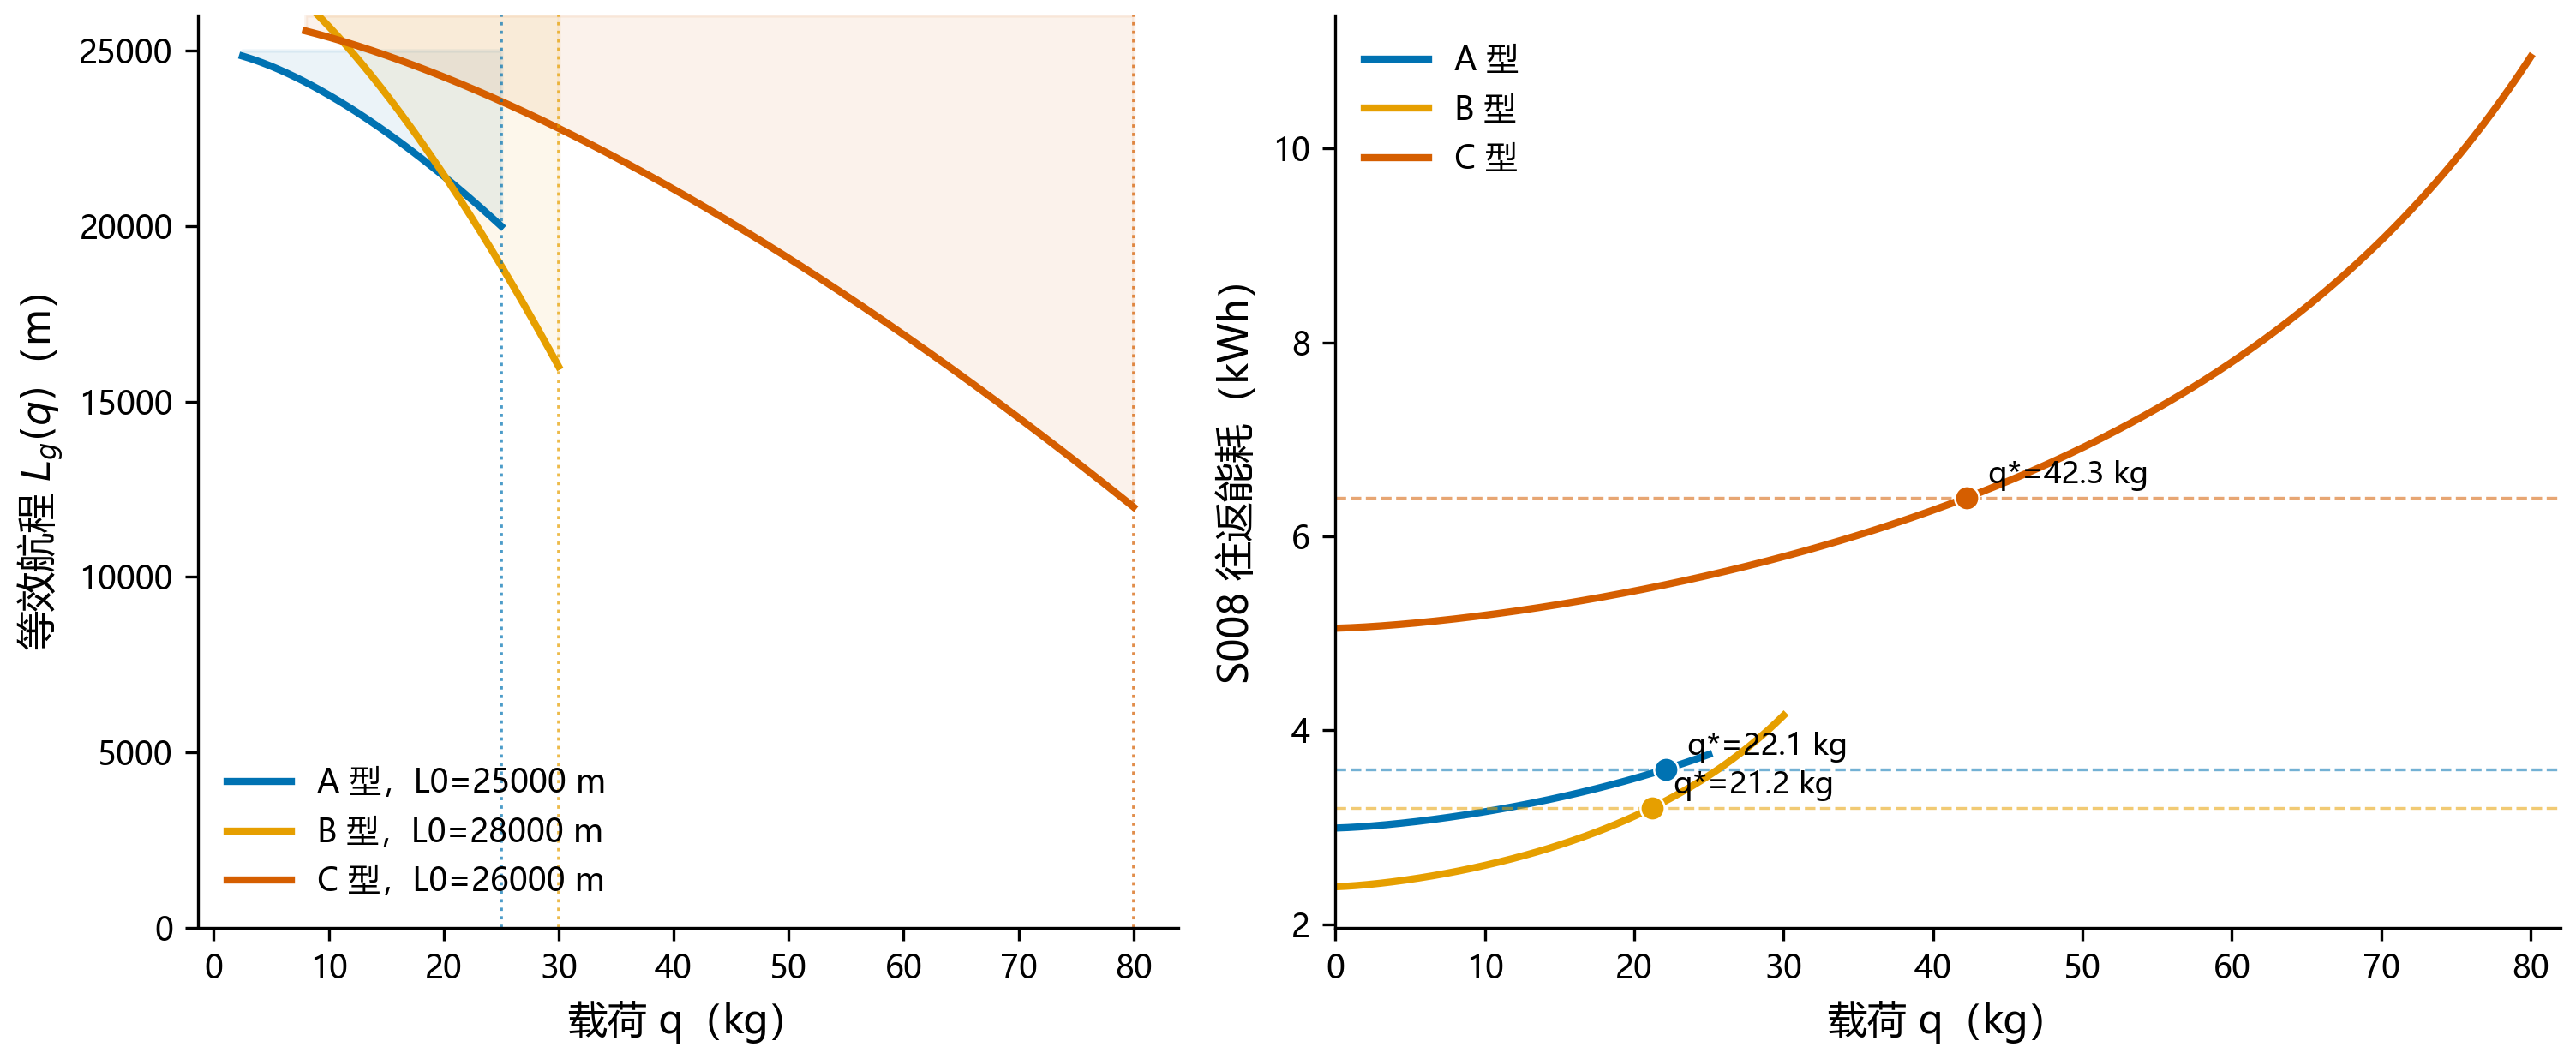
\includegraphics[width=0.96\textwidth]{figures/p1_lg_curve.png}
\caption{左：等效航程随载荷收缩曲线；右：三机型到 S008 往返能耗随载荷变化及能量上限交点}
\label{fig:lgcurve}
\end{figure}

\subsubsection{最大安全载荷求解}

对机型 $m$ 与服务区 $S_i$，总能耗随载荷 $q$ 单调递增，原因是等效航程随
$q$ 递减且爬升功递增。在可行区间内对 $q$ 二分求解
$E_{\mathrm{total}}(q)=(1-\rho)E_{\mathrm{use}}$，即得能量限制载荷，再与
质量上限、体积上限取最小，得到最大安全载荷 $q^*_{m,i}$。

\subsubsection{货箱组批模型}

各服务区货箱按机型与服务区分组，组批视为带容量约束的装箱问题：同一服务区
同一机型的货箱，按质量、体积与能耗装入最少架次，每架次往返于 O01 与单一
服务区。目标为最小化总架次数与总能耗，按式 \eqref{eq:bin} 表述。

\begin{equation}
\min \ \sum_{m,i} n_{m,i}, \qquad
\min \ \sum_{m,i}\sum_{k=1}^{n_{m,i}} E^{(k)}_{m,i}
\label{eq:bin}
\end{equation}

约束为每箱恰入一架次、架次质量体积能耗不超限、架次载荷不超过对应最大安全
载荷。

\subsection{模型求解}

对 A、B、C 三类机型逐区求最大安全载荷，结果如表 \ref{tab:qstar} 所示，其中
能量受限值用粗体标出，其余为质量或体积上限。A 型全部区域取质量上限 25\,kg；
B 型除 S008 因远距高差受能量约束降为约 28.9\,kg 外均取 30\,kg；C 型多数区域
取 80\,kg，而 S002、S003、S004、S008、S012 五个区域因航线较长或爬升较高，
受能量约束为 59.2 至 69.0\,kg。图 \ref{fig:qstar} 直观给出三机型各区域的载荷
对比，可见能量约束集中在 C 型远区。

\begin{table}[htbp]
\centering
\caption{各机型到各服务区的最大安全载荷（kg）}
\label{tab:qstar}
\resizebox{\textwidth}{!}{%
\begin{tabular}{l|ccccccccccccccc|c}
\toprule
机型 & S001 & S002 & S003 & S004 & S005 & S006 & S007 & S008 & S009 & S010 & S011 & S012 & S013 & S014 & S015 \\
\midrule
A & 25 & 25 & 25 & 25 & 25 & 25 & 25 & 25 & 25 & 25 & 25 & 25 & 25 & 25 & 25 \\
B & 30 & 30 & 30 & 30 & 30 & 30 & 30 & \textbf{28.9} & 30 & 30 & 30 & 30 & 30 & 30 & 30 \\
C & 80 & \textbf{69.0} & \textbf{68.4} & \textbf{63.9} & 80 & 80 & 80 & \textbf{59.2} & 80 & 80 & 80 & \textbf{68.2} & 80 & 80 & 80 \\
\bottomrule
\end{tabular}}
\end{table}

\begin{figure}[htbp]
\centering
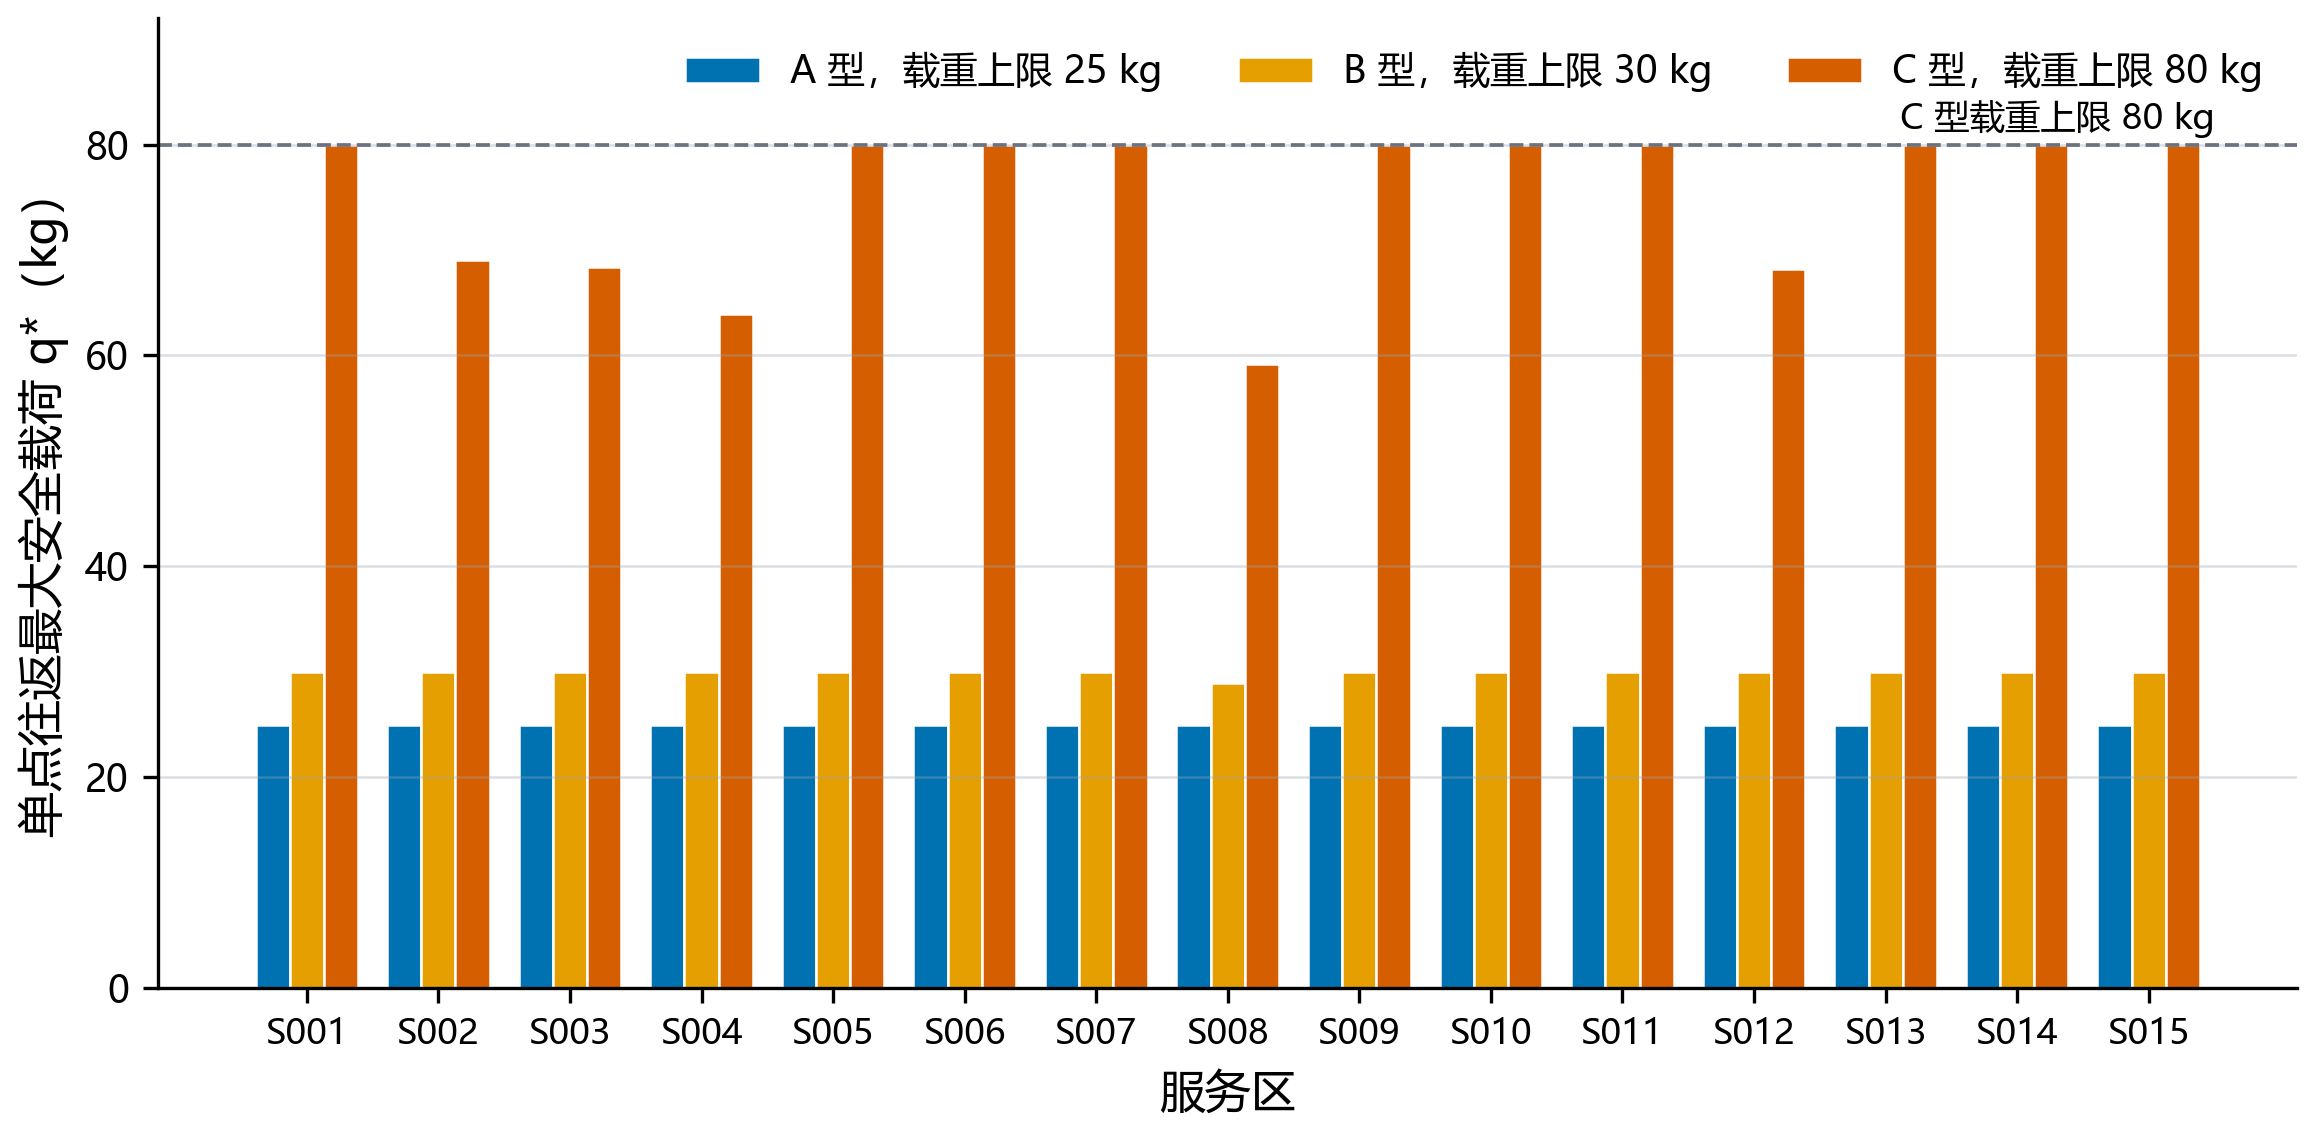
\includegraphics[width=0.84\textwidth]{figures/p1_qstar.png}
\caption{三机型在各服务区的最大安全载荷对比}
\label{fig:qstar}
\end{figure}

按式 \eqref{eq:bin} 组批，全网共 18 架次、总能耗 59.02\,kWh、总飞行时间约
32661\,s。表 \ref{tab:p1summary} 给出各服务区的组批概览：重载区由 C 型承担，
其中 S001 的 154\,kg 货箱分 2 架次完成；S009 至 S015 各 25\,kg 由 B 型单架次
送达。每架次的货箱编号、质量、体积、往返时间、能耗与返航荷电状态见《结果提交
模板》Q1 工作表；全部架次返航荷电状态均不低于 20\%，满足安全约束。

\begin{table}[htbp]
\centering
\caption{问题一各服务区组批概览}
\label{tab:p1summary}
\begin{tabular}{lcccc}
\toprule
服务区 & 货箱数 & 总质量(kg) & 架次数 & 能耗(kWh) \\
\midrule
S001 & 15 & 154 & 2 & 5.90 \\
S002 & 8 & 81 & 2 & 8.42 \\
S003 & 8 & 81 & 2 & 8.53 \\
S004 & 6 & 59 & 1 & 6.14 \\
S005--S008 & 22 & 208 & 4 & 16.03 \\
S009--S015 & 21 & 175 & 7 & 14.00 \\
\midrule
合计 & 80 & 758 & 18 & 59.02 \\
\bottomrule
\end{tabular}
\end{table}

图 \ref{fig:soc} 给出各架次按能耗升序的返航荷电状态，全部位于 20\% 安全
下限之上，最低约 23\%；重载 C 型架次能耗占比最高，返航荷电状态贴近下限，
其余架次保留更充分的余量。

\begin{figure}[htbp]
\centering
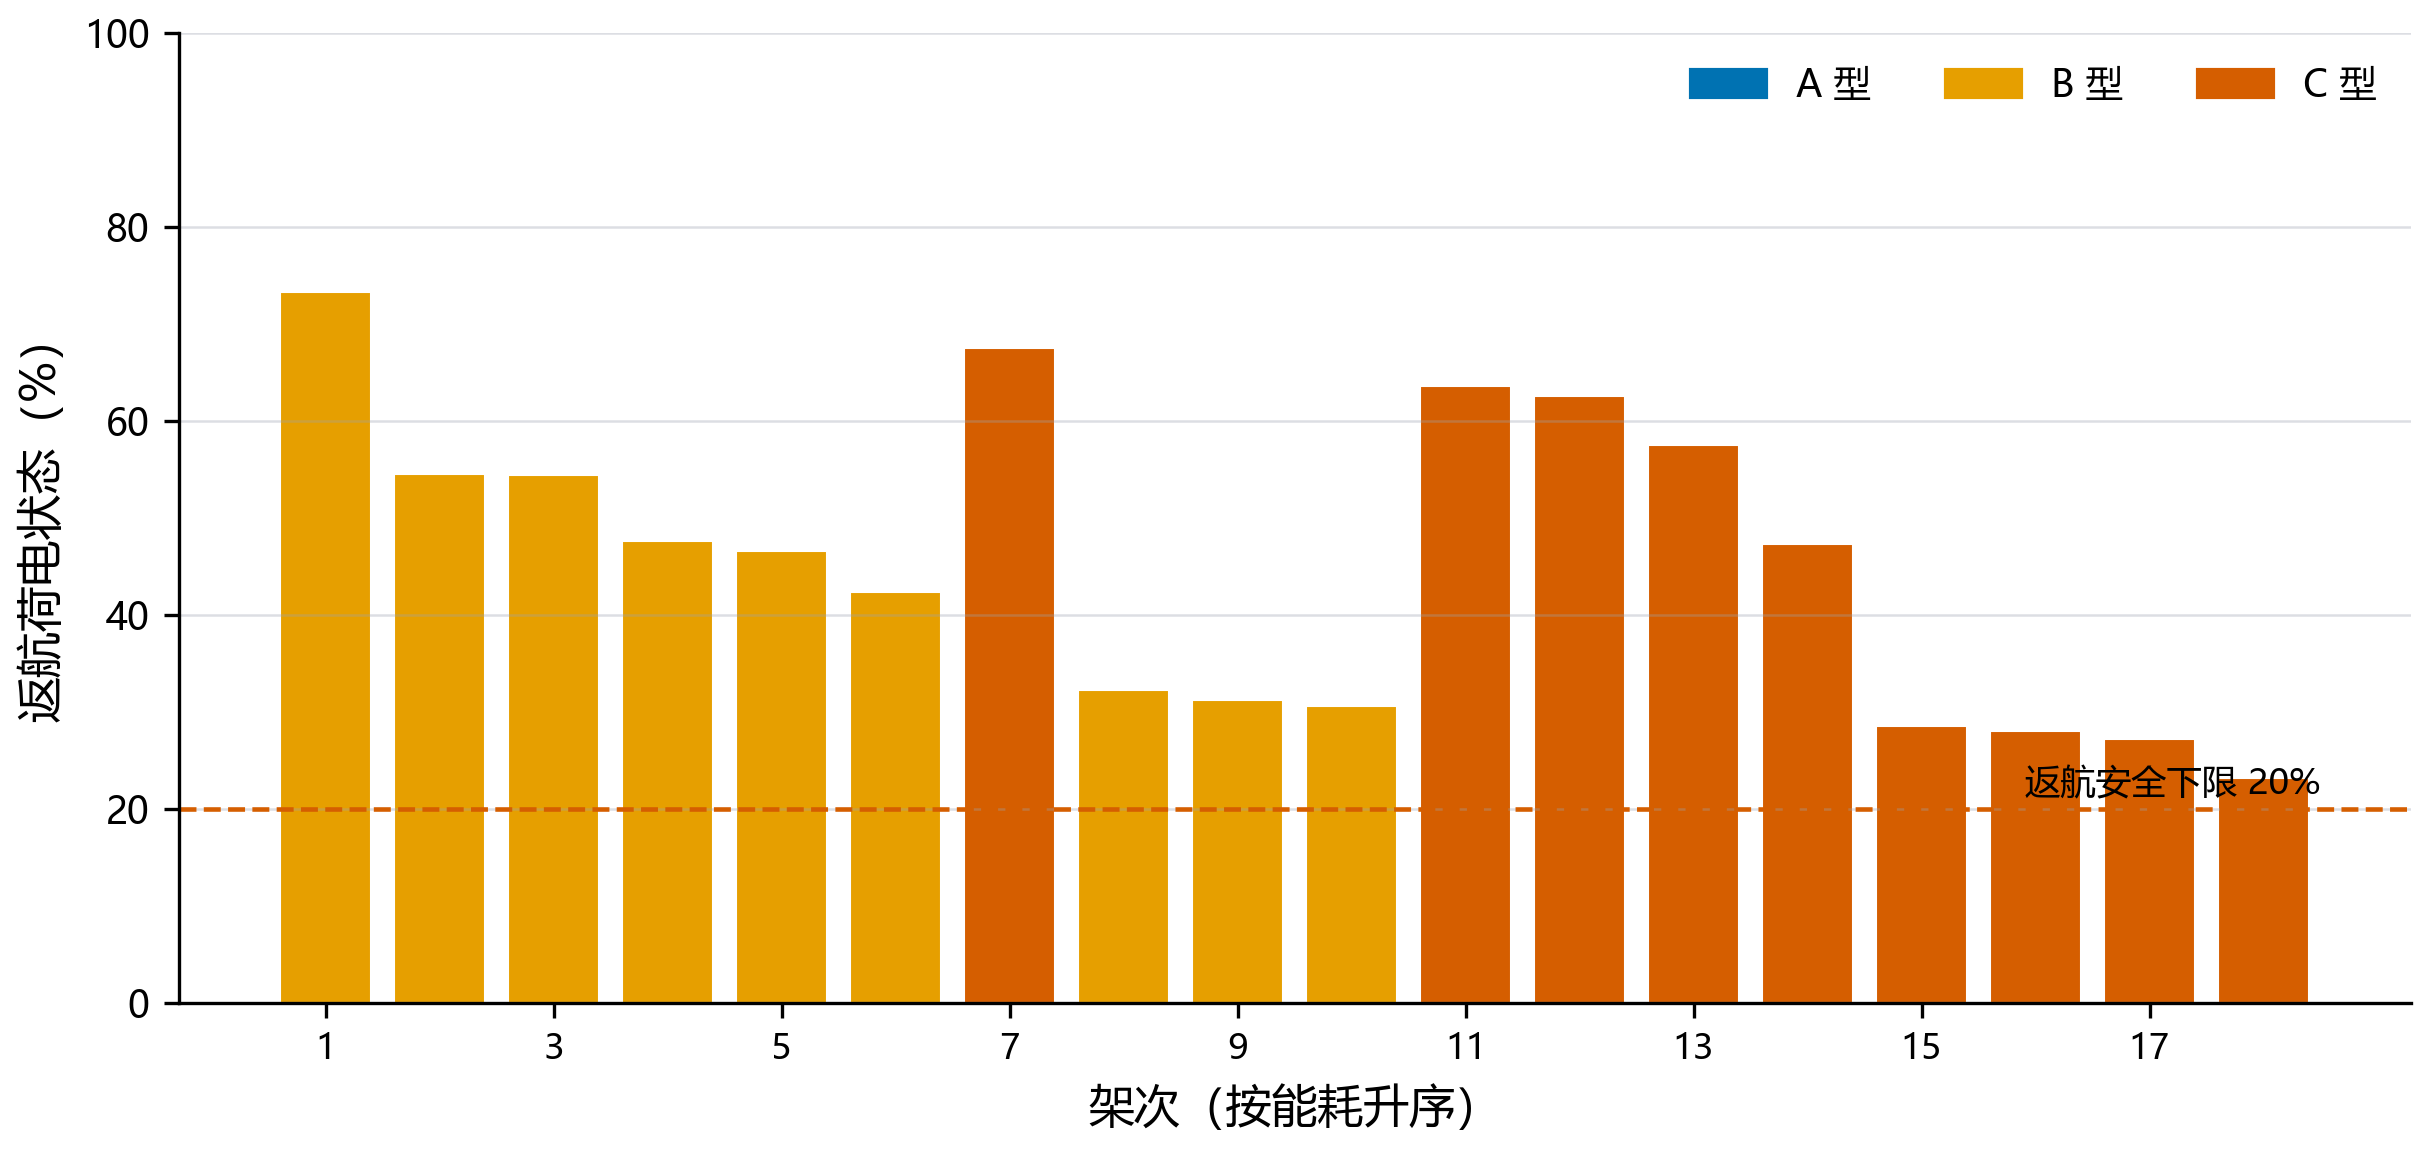
\includegraphics[width=0.9\textwidth]{figures/p1_soc.png}
\caption{问题一各架次返航荷电状态（虚线为 20\% 安全下限）}
\label{fig:soc}
\end{figure}

\subsection{结果分析}

\begin{enumerate}
\item \textbf{能量约束主导远区}：C 型到 S008 的最大安全载荷 59.2\,kg 为全网
最低，对应最长航线与最大爬升的组合；A、B 型因质量上限较低，能量约束几乎不
生效，仅 B 型到 S008 略受约束。这说明远距加高差是山区无人机投送的关键瓶颈。
\item \textbf{组批节省架次}：重载区用 C 型多装，单架 63.9 至 80\,kg，轻载区用
B 型单架直送，18 架次即完成全部 80 箱，架次利用率较高。
\item \textbf{安全余量与效率权衡}：安全余量比例 $\rho$ 从 0.2 增大到 0.35 时，
架次数由 18 增至 25，能耗由 59.02 升至 77.63\,kWh，增幅约 31.5%；$\rho$ 由
0.35 增至 0.40 时架次数不变而能耗由 77.63 降至 74.62\,kWh，说明该区间发生
机型结构切换，部分 C 型远区架次改由更经济的组合完成。详细的扫描结果见第
\ref{sec:sens}节。
\end{enumerate}
% 问题二
\section{问题二：异构无人机多点多架次调度}
\label{sec:p2}

\subsection{问题分析}

问题二要求把 80 个货箱从 O01 运往 15 个服务区，机队为 A、B、C 三类共 8 架
无人机，即 A 型 4 架、B 型 2 架、C 型 2 架，配 14 组共享电池，即 A 型 6、B 型 4、C 型 4。难点有
四个方面。其一为异构性，三类机型在载荷、速度、等效航程与能耗上差异显著，
重载长航任务几乎只能由 C 型承担，C 型成为瓶颈。其二为时限约束，货箱分首飞批
与普通批两类，首飞批时限为 3600、7200、10800\,s 三档，普通批不超过 18000\,s，
医疗货箱另有严时限。其三为资源耦合，无人机与电池双重资源决定架次能否按时
出发，电池充电需按两阶段曲线排程。其四为多目标，架次数、总能耗与总完工时间
三者存在权衡。

\subsection{模型建立}

\subsubsection{决策变量}

以架次为决策单元。架次由机型、航线与货箱集合三元组刻画，调度器输出每个架次
的起降时刻、所用无人机与电池编号。全网货箱集合被划分为互不重叠的架次集合，
每一架次依次访问若干服务区。

\subsubsection{调度规则}

按截止期优先规则对架次排序：架次的关键时刻取其所载货箱的最早时限，即首飞批
优先于普通批，医疗货箱最高优先；同关键时刻按货箱总优先级降序。对每个架次，
在空闲且型号匹配的无人机与满电电池中取最早可用组合，出发时刻按式
\eqref{eq:start} 计算。

\begin{equation}
t_{\mathrm{start}}=\max\{r_k,\ t_{\mathrm{free}}(uav),\ t_{\mathrm{ready}}(bat)\}
+ t_{\mathrm{prep}}
\label{eq:start}
\end{equation}

其中 $r_k$ 为架次释放时刻，$t_{\mathrm{free}}$ 为无人机返场时刻，
$t_{\mathrm{ready}}$ 为电池充满时刻，$t_{\mathrm{prep}}$ 为起飞准备时长，按
机型取 300 加 30 乘以货箱数，单位秒。架次能耗按式 \eqref{eq:lg} 至式
\eqref{eq:eup} 计算，返航后电池进入两阶段充电队列。

\subsubsection{目标函数}

综合四项目标并加权，按式 \eqref{eq:obj2} 表述。

\begin{equation}
\begin{aligned}
\min\ J ={} & w_t \sum_k \frac{\tau_k p_k}{24} + w_f\, N_f \\
& + w_m\, C_{\max} + w_e\, E_{\mathrm{tot}}
\end{aligned}
\label{eq:obj2}
\end{equation}

其中 $\tau_k$ 为架次内货箱的超期时间，$p_k$ 为货箱优先级，$N_f$ 为架次数，
$C_{\max}=\max_k t_{\mathrm{return},k}$ 为完工时间，$E_{\mathrm{tot}}$ 为总
能耗。硬约束为首飞批货箱与医疗货箱必须满足时限，违反即解不可行；软约束为
普通批超期的加权惩罚。

\subsubsection{求解算法}

求解分三步进行。步骤 1 为初始解生成，按时限贪心组批，即先按服务区与机型
聚类，再按容量装入架次，并把每服务区的紧急箱（首飞批与医疗箱）拆出为优先
架次。步骤 2 为种群进化，采用遗传算法，个体为架次集合，目标函数即式
\eqref{eq:obj2}；五种变异算子分别执行架次合并、架次拆分、区段换序、
跨架次移箱与换机型，交叉算子随机选取货箱子集直接继承父代并对其余货箱贪心
插回，精英保留两个最优个体。步骤 3 为调度解码，按截止期优先排序架次，耦合
无人机与电池双资源就绪队列求可行派单，硬约束违反计以巨额惩罚。以固定随机
种子运行，结果可复现。对照组另以模拟退火（货箱移动、交换、合并、拆分与区段
重排五算子）扫描四组权重，用于多目标权衡分析。遗传算法主要参数如表
\ref{tab:gaparams} 所示。

\begin{table}[htbp]
\centering
\caption{遗传算法主要参数}
\label{tab:gaparams}
\begin{tabular}{lcl}
\toprule
参数 & 取值 & 说明 \\
\midrule
种群规模 & 12 & 每代个体数 \\
进化代数 & 150 & 终止条件 \\
变异概率 & 0.45 & 每个体发生变异的概率 \\
变异算子 & 5 类 & 合并、拆分、区段换序、跨架次移箱、换机型 \\
交叉算子 & 子集继承 & 随机子集直传父代，其余贪心插回 \\
精英保留 & 2 & 每代最优个体直接进入下一代 \\
锦标赛规模 & 2 & 选择压力 \\
随机种子 & 7 & 结果可复现 \\
\bottomrule
\end{tabular}
\end{table}

\subsection{模型求解与结果}

\subsubsection{多目标权衡}

在算法进化环节，对同一优化问题并行考察模拟退火、遗传算法、自适应大邻域搜索、
禁忌搜索与 GRASP 五类元启发式框架，并对禁忌搜索执行多权重--多种子强化搜索
（四组权重 $\times$ 三个种子、总预算 600\,s），得到收敛的零迟到 Pareto 前沿，
如表 \ref{tab:pareto} 所示。本文选取完工口径冠军：26 架次、完工约 6960\,s、
能耗 70.71\,kWh，较原遗传算法均衡方案（24 架次、8342\,s、77.31\,kWh）完工提前
约 1382\,s（16.6\%）、能耗降低约 6.6\,kWh；若以能耗为先，21 架次方案约
7837\,s/62.46\,kWh，19 架次方案约 7920\,s/60.40\,kWh。三目标不可同时最优，
故按完工口径选取零迟到的 Tabu 冠军方案。

\begin{table}[htbp]
\centering
\caption{问题二多目标权衡（Tabu 冠军与对照权重方案）}
\label{tab:pareto}
\begin{tabular}{lcccc}
\toprule
方案（算法） & 架次数 & 完工时间(s) & 能耗(kWh) & 加权迟到 \\
\midrule
完工冠军（Tabu，本文选取） & \textbf{26} & \textbf{6960} & \textbf{70.71} & \textbf{0} \\
节能均衡（Tabu） & 21 & 7837 & 62.46 & 0 \\
最低能耗（Tabu） & 19 & 7920 & 60.40 & 0 \\
原均衡（GA，对照） & 24 & 8342 & 77.31 & 0 \\
\bottomrule
\end{tabular}
\end{table}

图 \ref{fig:pareto2d} 以气泡大小表示架次数，直观显示各方案在完工时间与
总能耗平面上的权衡位置；本文完工冠军在零迟到前提下以最少时间换取最优完工，
节能备选则以更低能耗换取更长完工。

\begin{figure}[htbp]
\centering
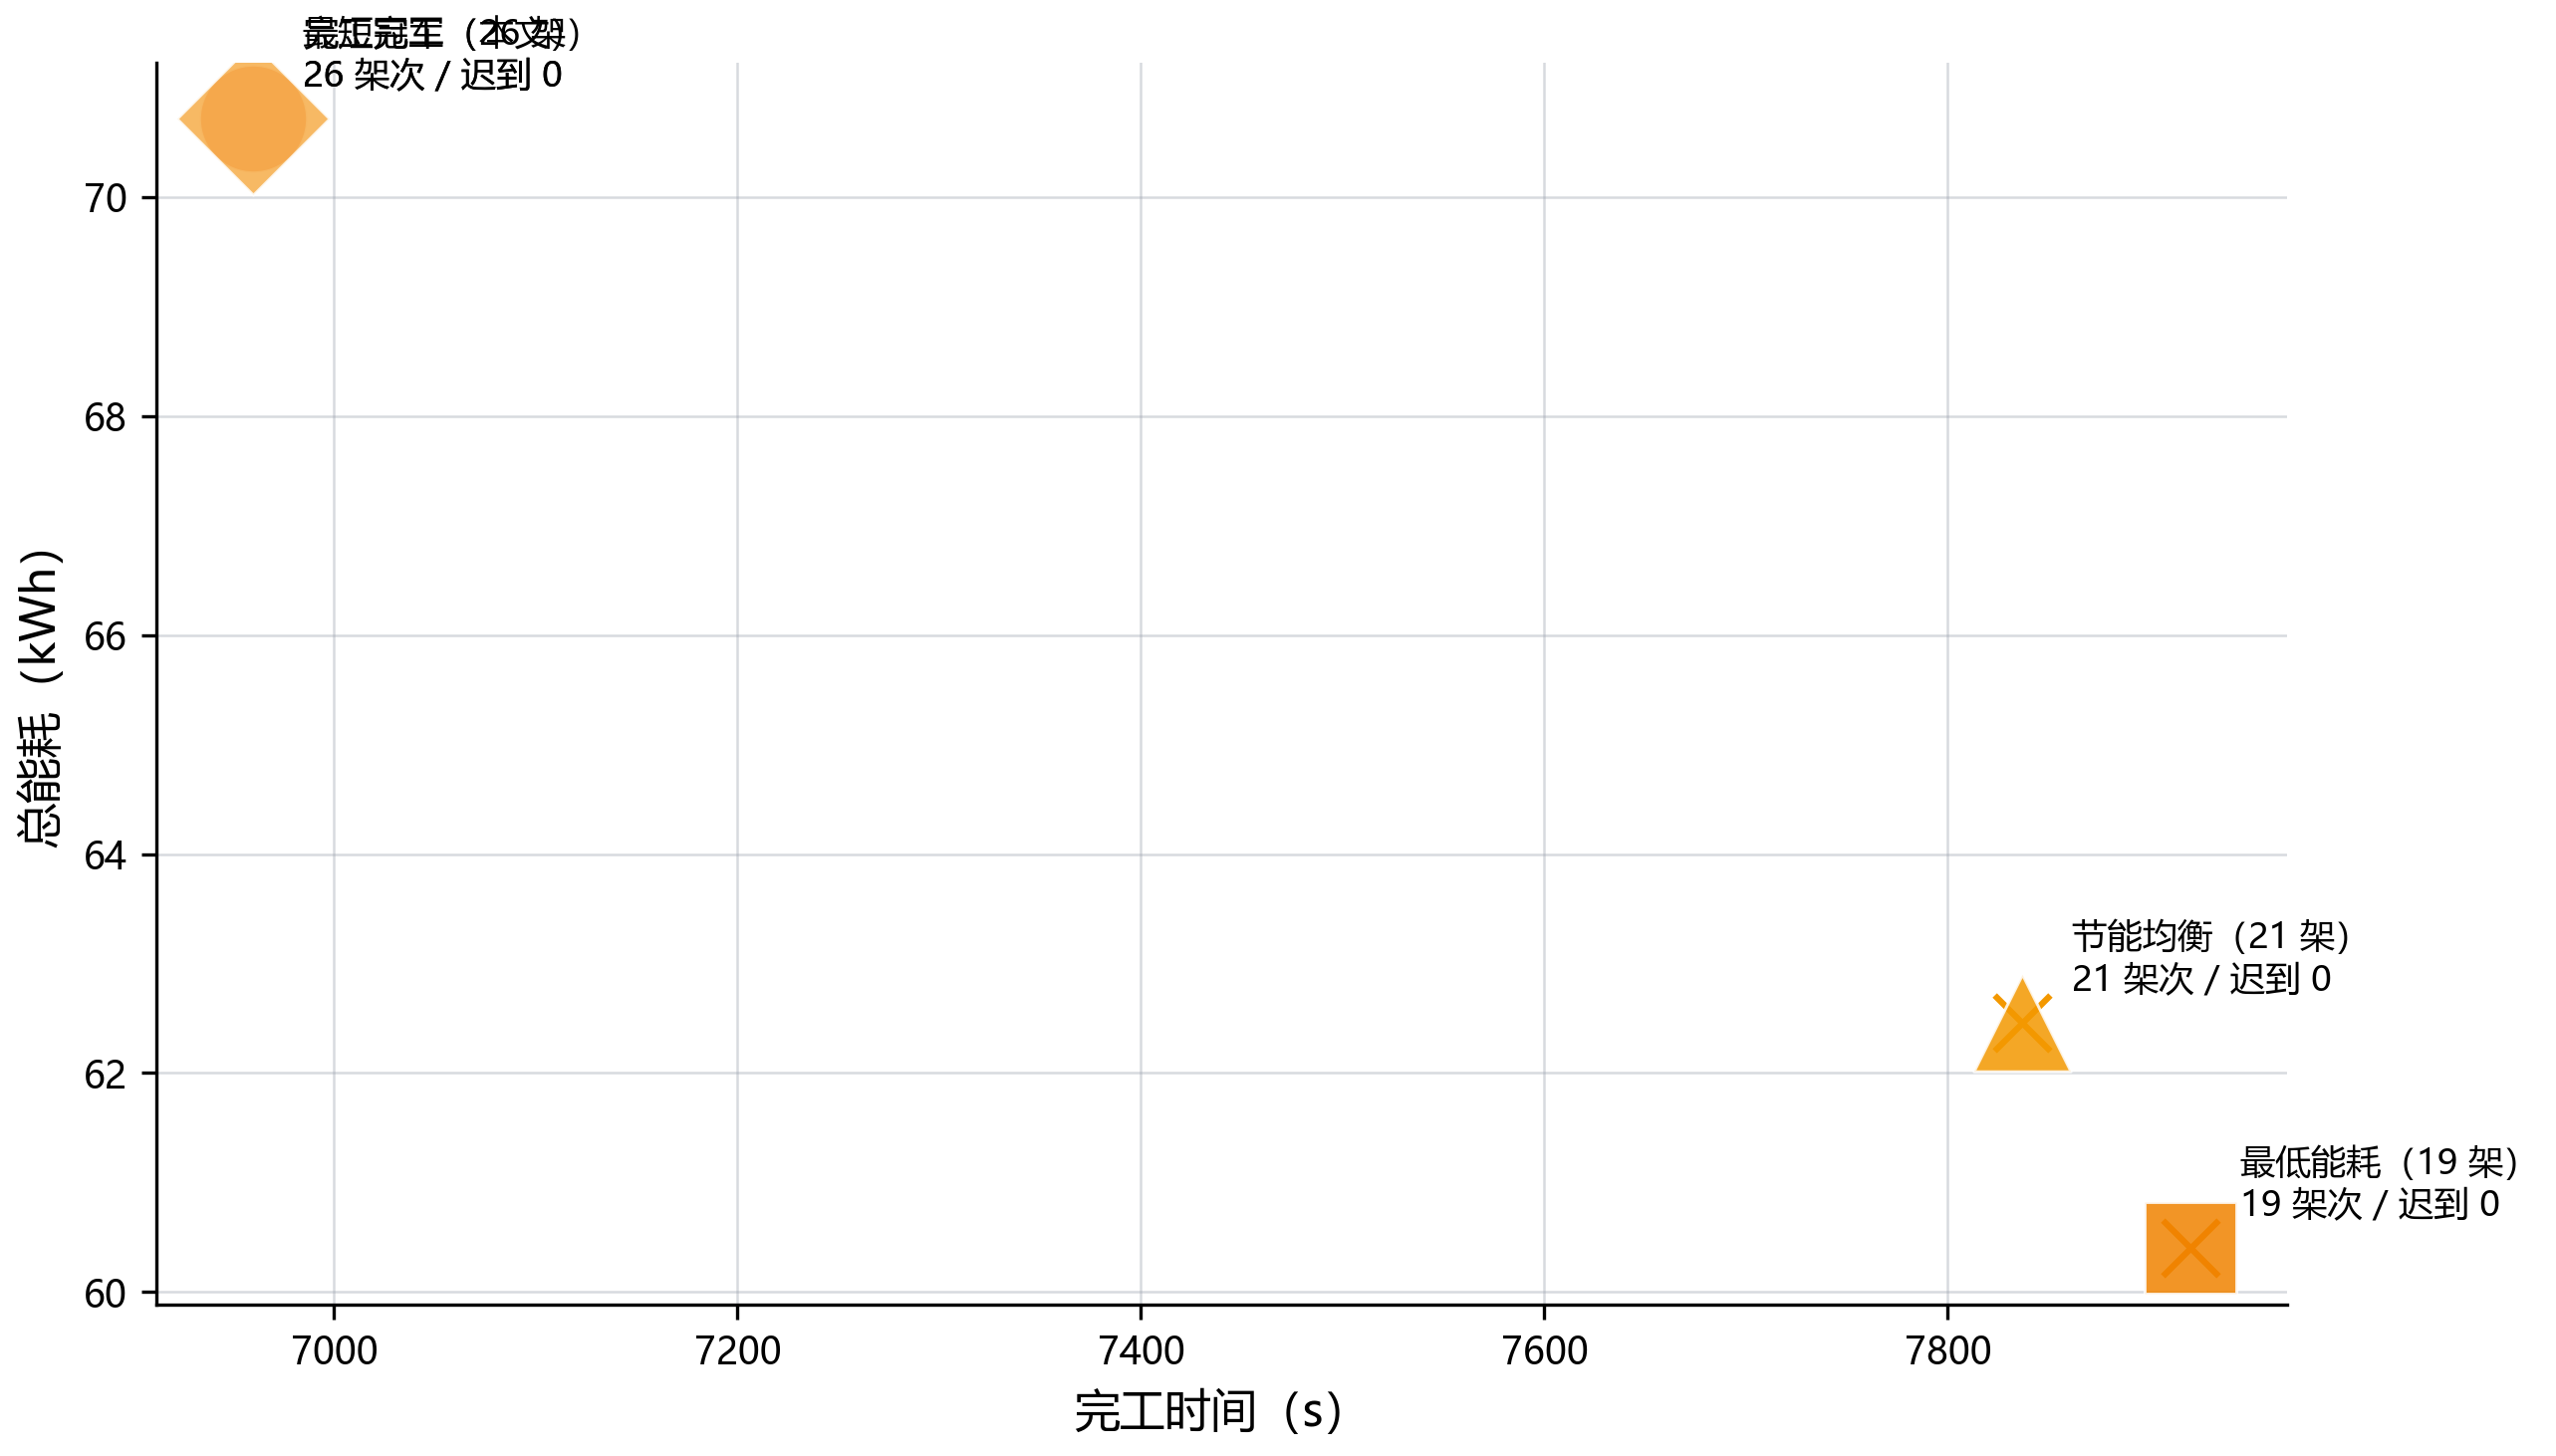
\includegraphics[width=0.86\textwidth]{figures/p2_pareto2d.png}
\caption{问题二多目标权衡（气泡大小为架次数）}
\label{fig:pareto2d}
\end{figure}

\subsubsection{均衡调度方案}

均衡方案共 26 架次，其中 A 型 12、B 型 7、C 型 7，全部 80 箱按时交付，即硬
约束满足且加权迟到为零，完工时间约 6960\,s，总能耗 70.71\,kWh。图
\ref{fig:p2net} 给出 26 架次在数字高程背景上的航线网络，可见 C 型航线构成
远距重载走廊，A、B 型负责短途轻载区；表 \ref{tab:p2flights} 给出架次明细，
图 \ref{fig:p2gantt} 给出各无人机的时间线，完整逐箱交付时刻见《结果提交
模板》Q2 工作表。

\begin{figure}[htbp]
\centering
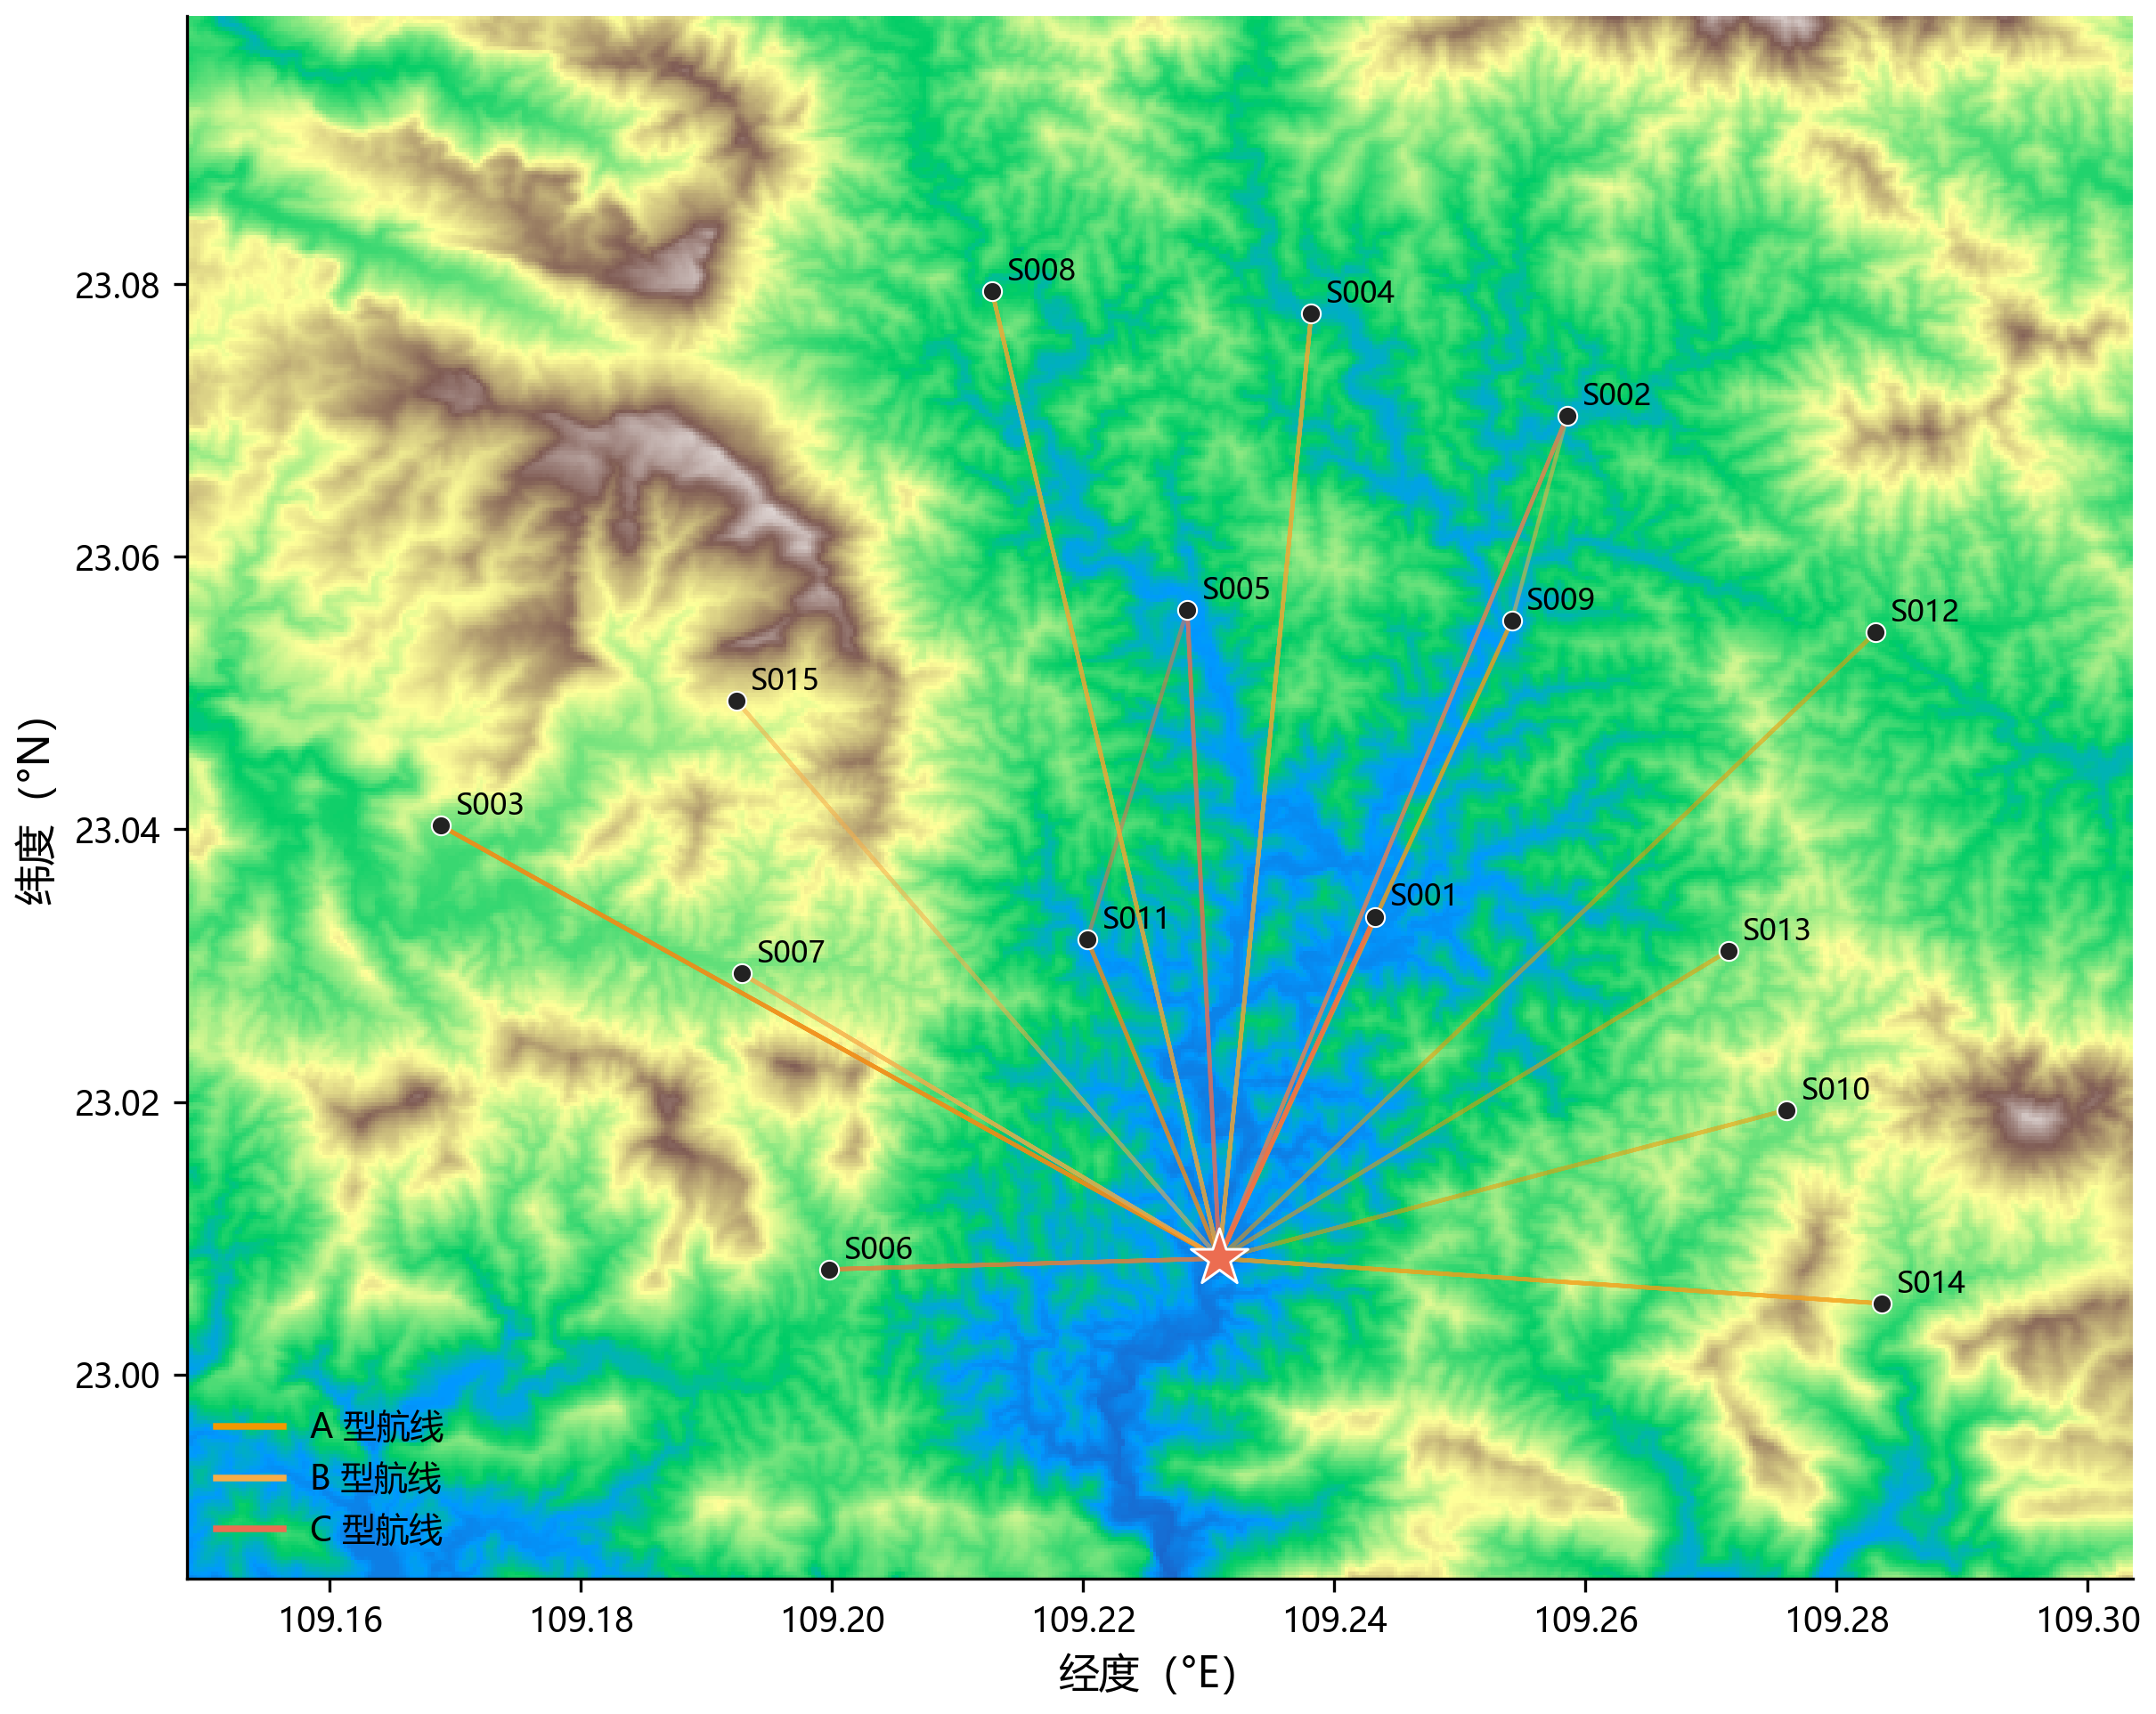
\includegraphics[width=0.82\textwidth]{figures/p2_network.png}
\caption{问题二均衡方案航线网络（按机型着色）}
\label{fig:p2net}
\end{figure}

\begin{table}[htbp]
\centering
\caption{问题二均衡调度方案（26 架次）}
\label{tab:p2flights}
\small
\begin{tabular}{ccccccc}
\toprule
架次 & 机型 & 无人机 & 开始(s) & 返回(s) & 能耗(kWh) & 航线 \\
\midrule
f24 & C & U08 & 0 & 1558 & 2.60 & S006 \\
f34 & C & U07 & 0 & 1559 & 2.99 & S001 \\
f18 & C & U08 & 1558 & 3595 & 5.52 & S002 \\
f17 & C & U07 & 1559 & 2986 & 2.40 & S001 \\
f23 & C & U07 & 2986 & 4926 & 4.39 & S005 \\
f20 & C & U08 & 3595 & 5949 & 5.46 & S003 \\
f05 & C & U07 & 4926 & 6960 & 3.81 & S005至S011 \\
\midrule
f07 & B & U06 & 0 & 1621 & 1.77 & S007 \\
f14 & B & U05 & 0 & 1861 & 1.99 & S014 \\
f35 & B & U06 & 1621 & 3182 & 1.69 & S007 \\
f02 & B & U05 & 1861 & 3825 & 2.63 & S002至S009 \\
f15 & B & U06 & 3182 & 5005 & 2.30 & S015 \\
f22 & B & U05 & 3825 & 5745 & 3.03 & S004 \\
f26 & B & U06 & 5005 & 6896 & 2.76 & S008 \\
\midrule
f01 & A & U01 & 0 & 1310 & 1.26 & S001 \\
f03 & A & U02 & 0 & 2310 & 3.03 & S003 \\
f06 & A & U03 & 0 & 1310 & 1.31 & S006 \\
f10 & A & U04 & 0 & 1649 & 1.95 & S010 \\
f12 & A & U01 & 1310 & 3357 & 2.91 & S012 \\
f04 & A & U03 & 1310 & 3487 & 3.08 & S004 \\
f31 & A & U04 & 1649 & 3255 & 1.94 & S013 \\
f32 & A & U02 & 2310 & 4291 & 2.27 & S014 \\
f21 & A & U04 & 3255 & 5505 & 3.08 & S003 \\
f08 & A & U01 & 3357 & 5458 & 3.14 & S008 \\
f09 & A & U03 & 3746 & 5432 & 2.25 & S009 \\
f11 & A & U02 & 4291 & 5507 & 1.15 & S011 \\
\bottomrule
\end{tabular}
\end{table}

\begin{figure}[htbp]
\centering
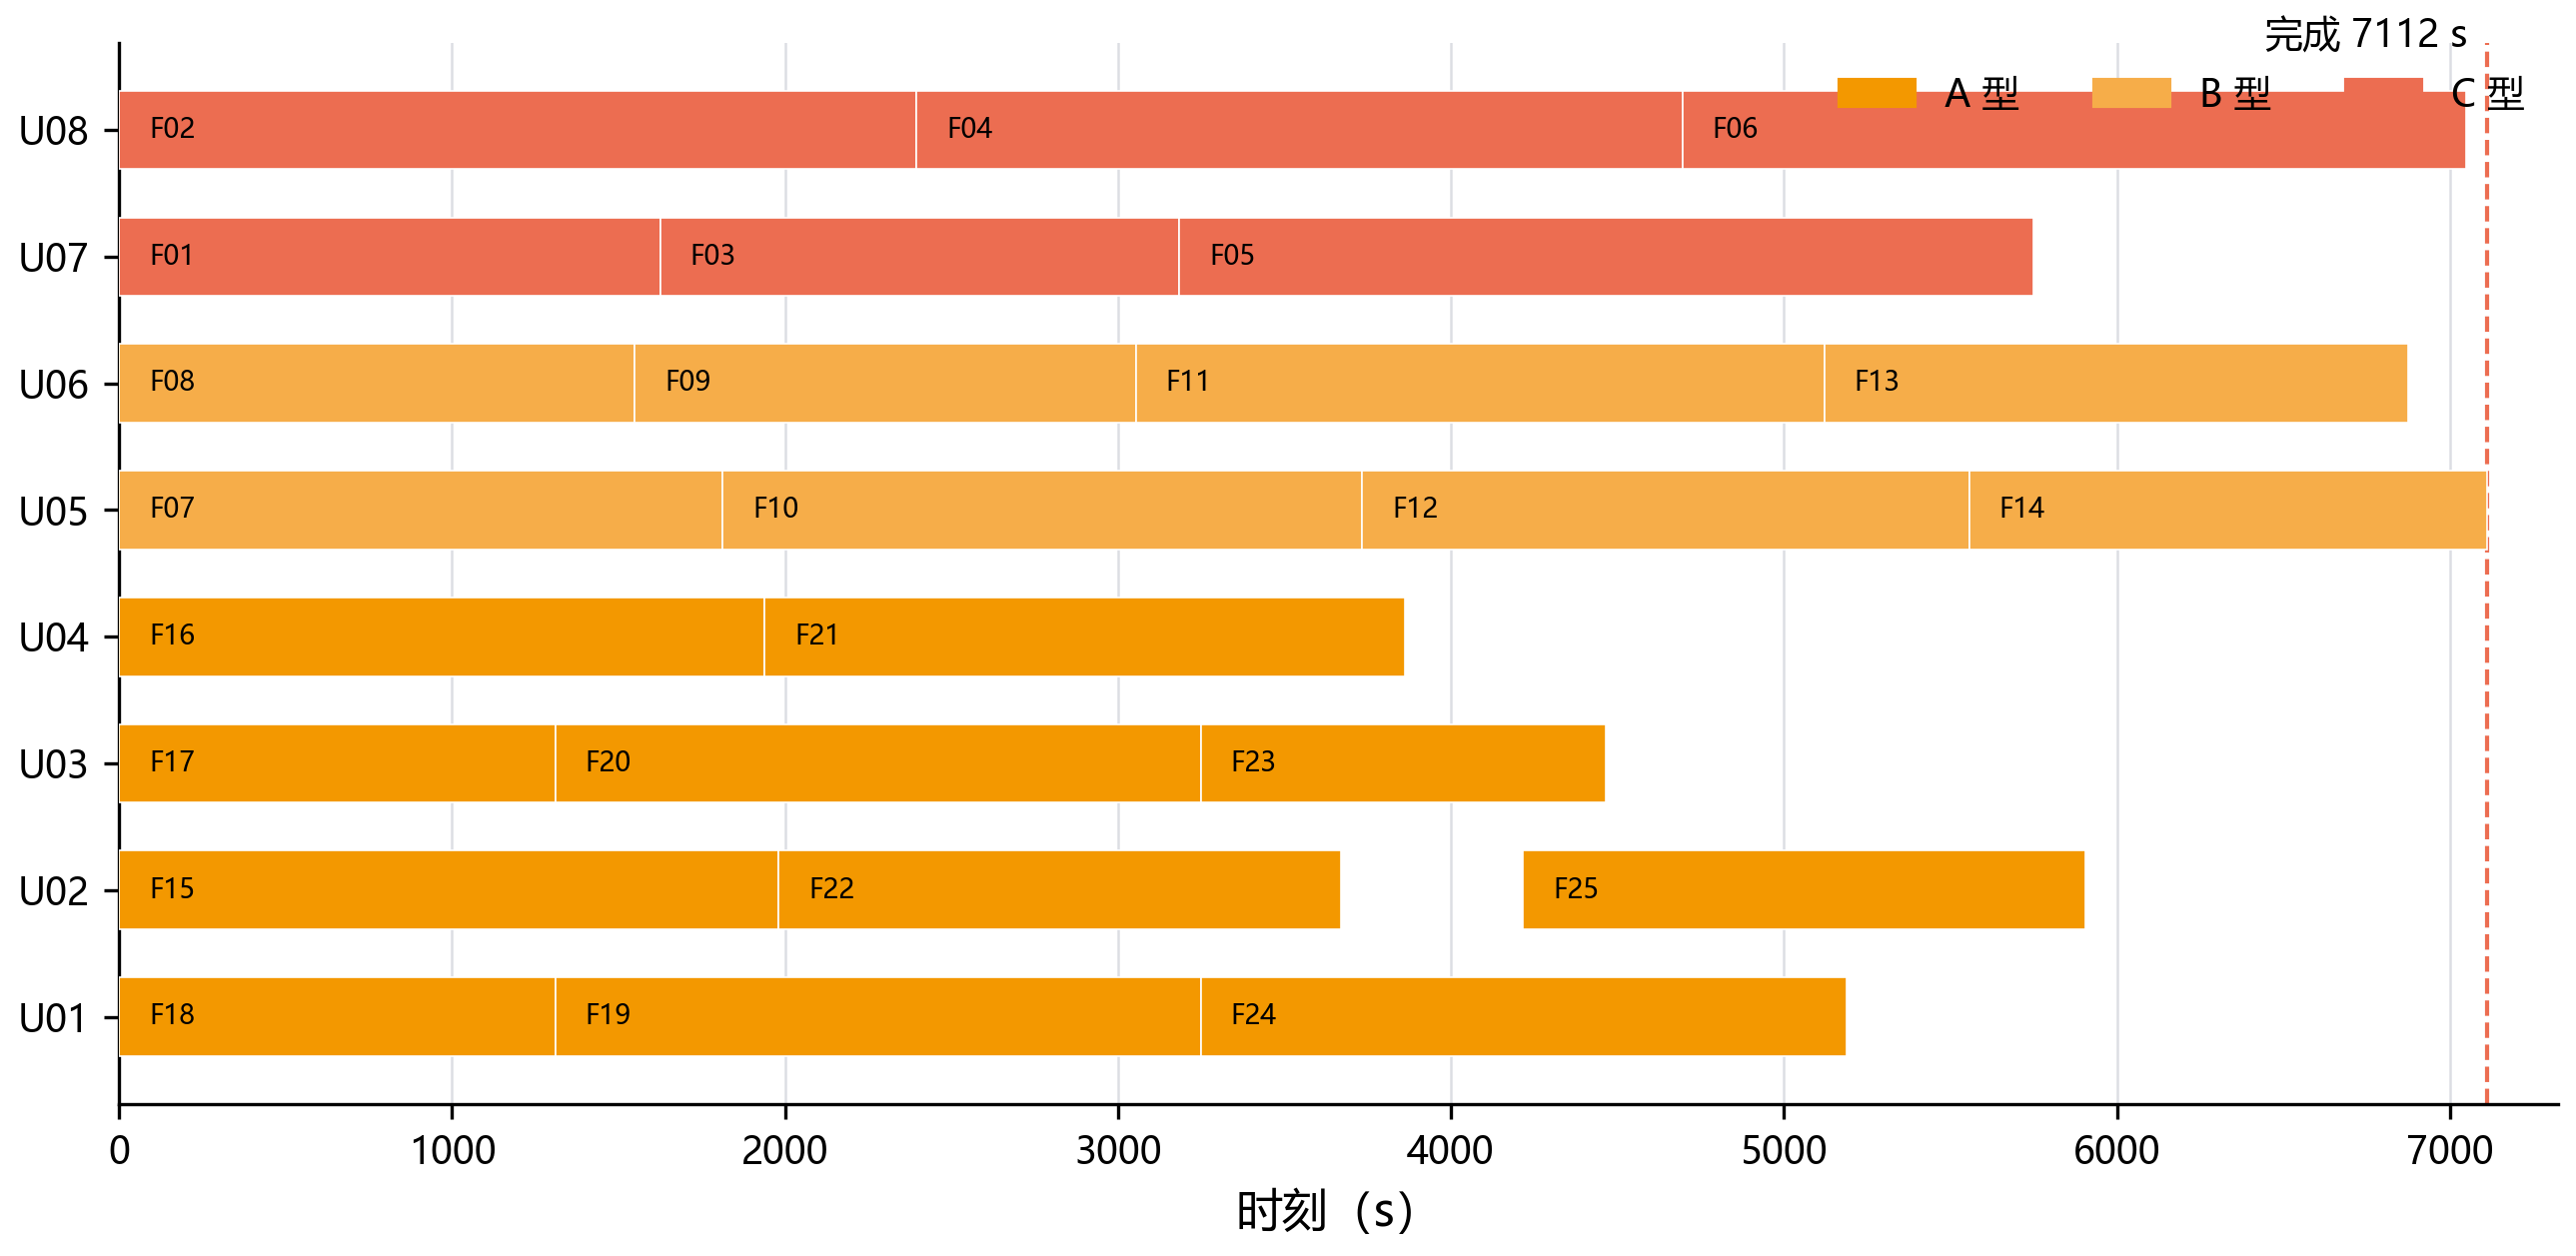
\includegraphics[width=0.95\textwidth]{figures/p2_gantt.png}
\caption{问题二均衡方案的运输任务甘特图（按无人机分泳道）}
\label{fig:p2gantt}
\end{figure}

\subsection{结果分析}

\begin{enumerate}
\item \textbf{C 型瓶颈}：7 个 C 架次承载了主要重载区任务，U07 与 U08 两架
C 型无人机几乎连续出勤至约 6960\,s，是完工时间的主要决定因素；A、B 型负责
轻载区与短途，链条明显更短，与远距重载只能由 C 型承担的物理规律一致。
\item \textbf{电池轮换充分}：共享电池在 26 架次中轮换，未出现电池短缺导致的
等待，说明电池数量不是瓶颈。图 \ref{fig:battery} 给出 14 组电池的任务段与
充电段时间线，充电按两阶段曲线，即低荷电快充后在 0.9 荷电以上转入慢充，使
电池在架次间隙即可恢复满电。

\begin{figure}[htbp]
\centering
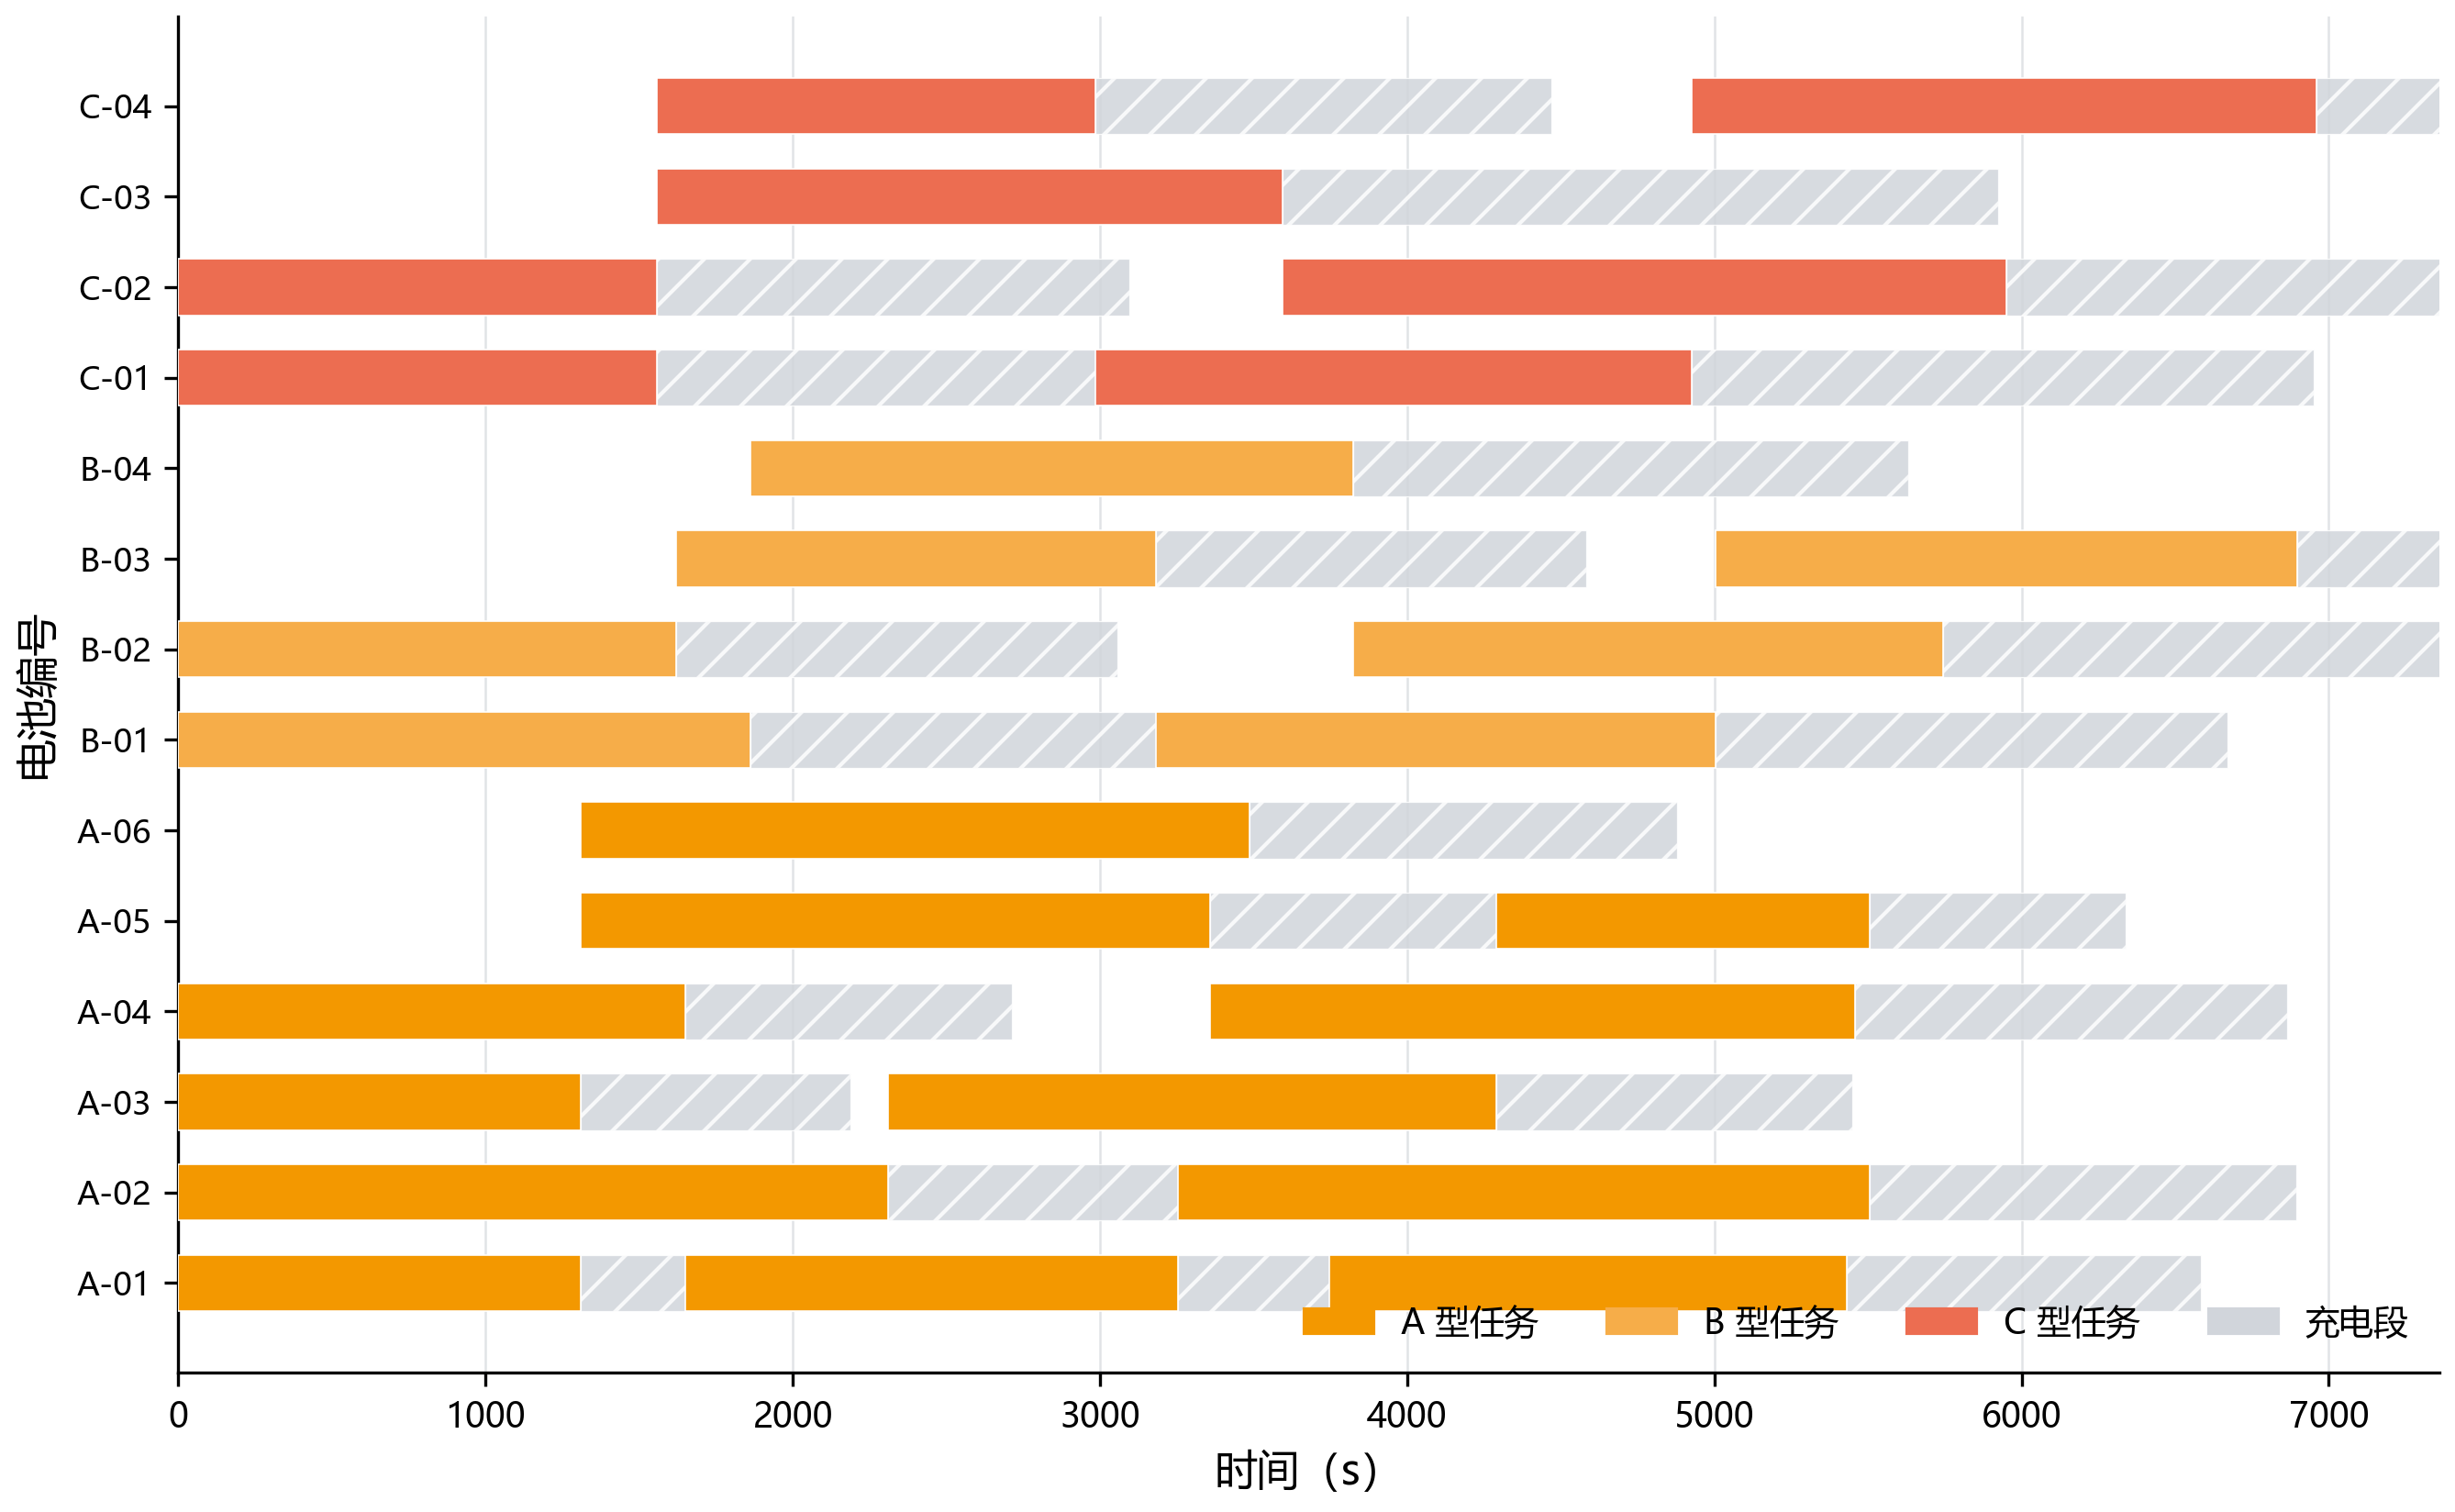
\includegraphics[width=0.98\textwidth]{figures/p2_battery.png}
\caption{14 组共享电池的任务与充电时间线（斜纹为充电段）}
\label{fig:battery}
\end{figure}

\item \textbf{时限全部满足}：首飞批货箱由首波架次优先送达，医疗货箱全部按
首飞批时限交付，普通批无超期。图 \ref{fig:delivery} 给出 80 箱的交付时刻与
配送时限散点，全部落在 45° 斜线以下，即交付不迟于时限；最紧裕度出现在
S004 服务区的最晚班次，系该区末班抵达所致。

\begin{figure}[htbp]
\centering
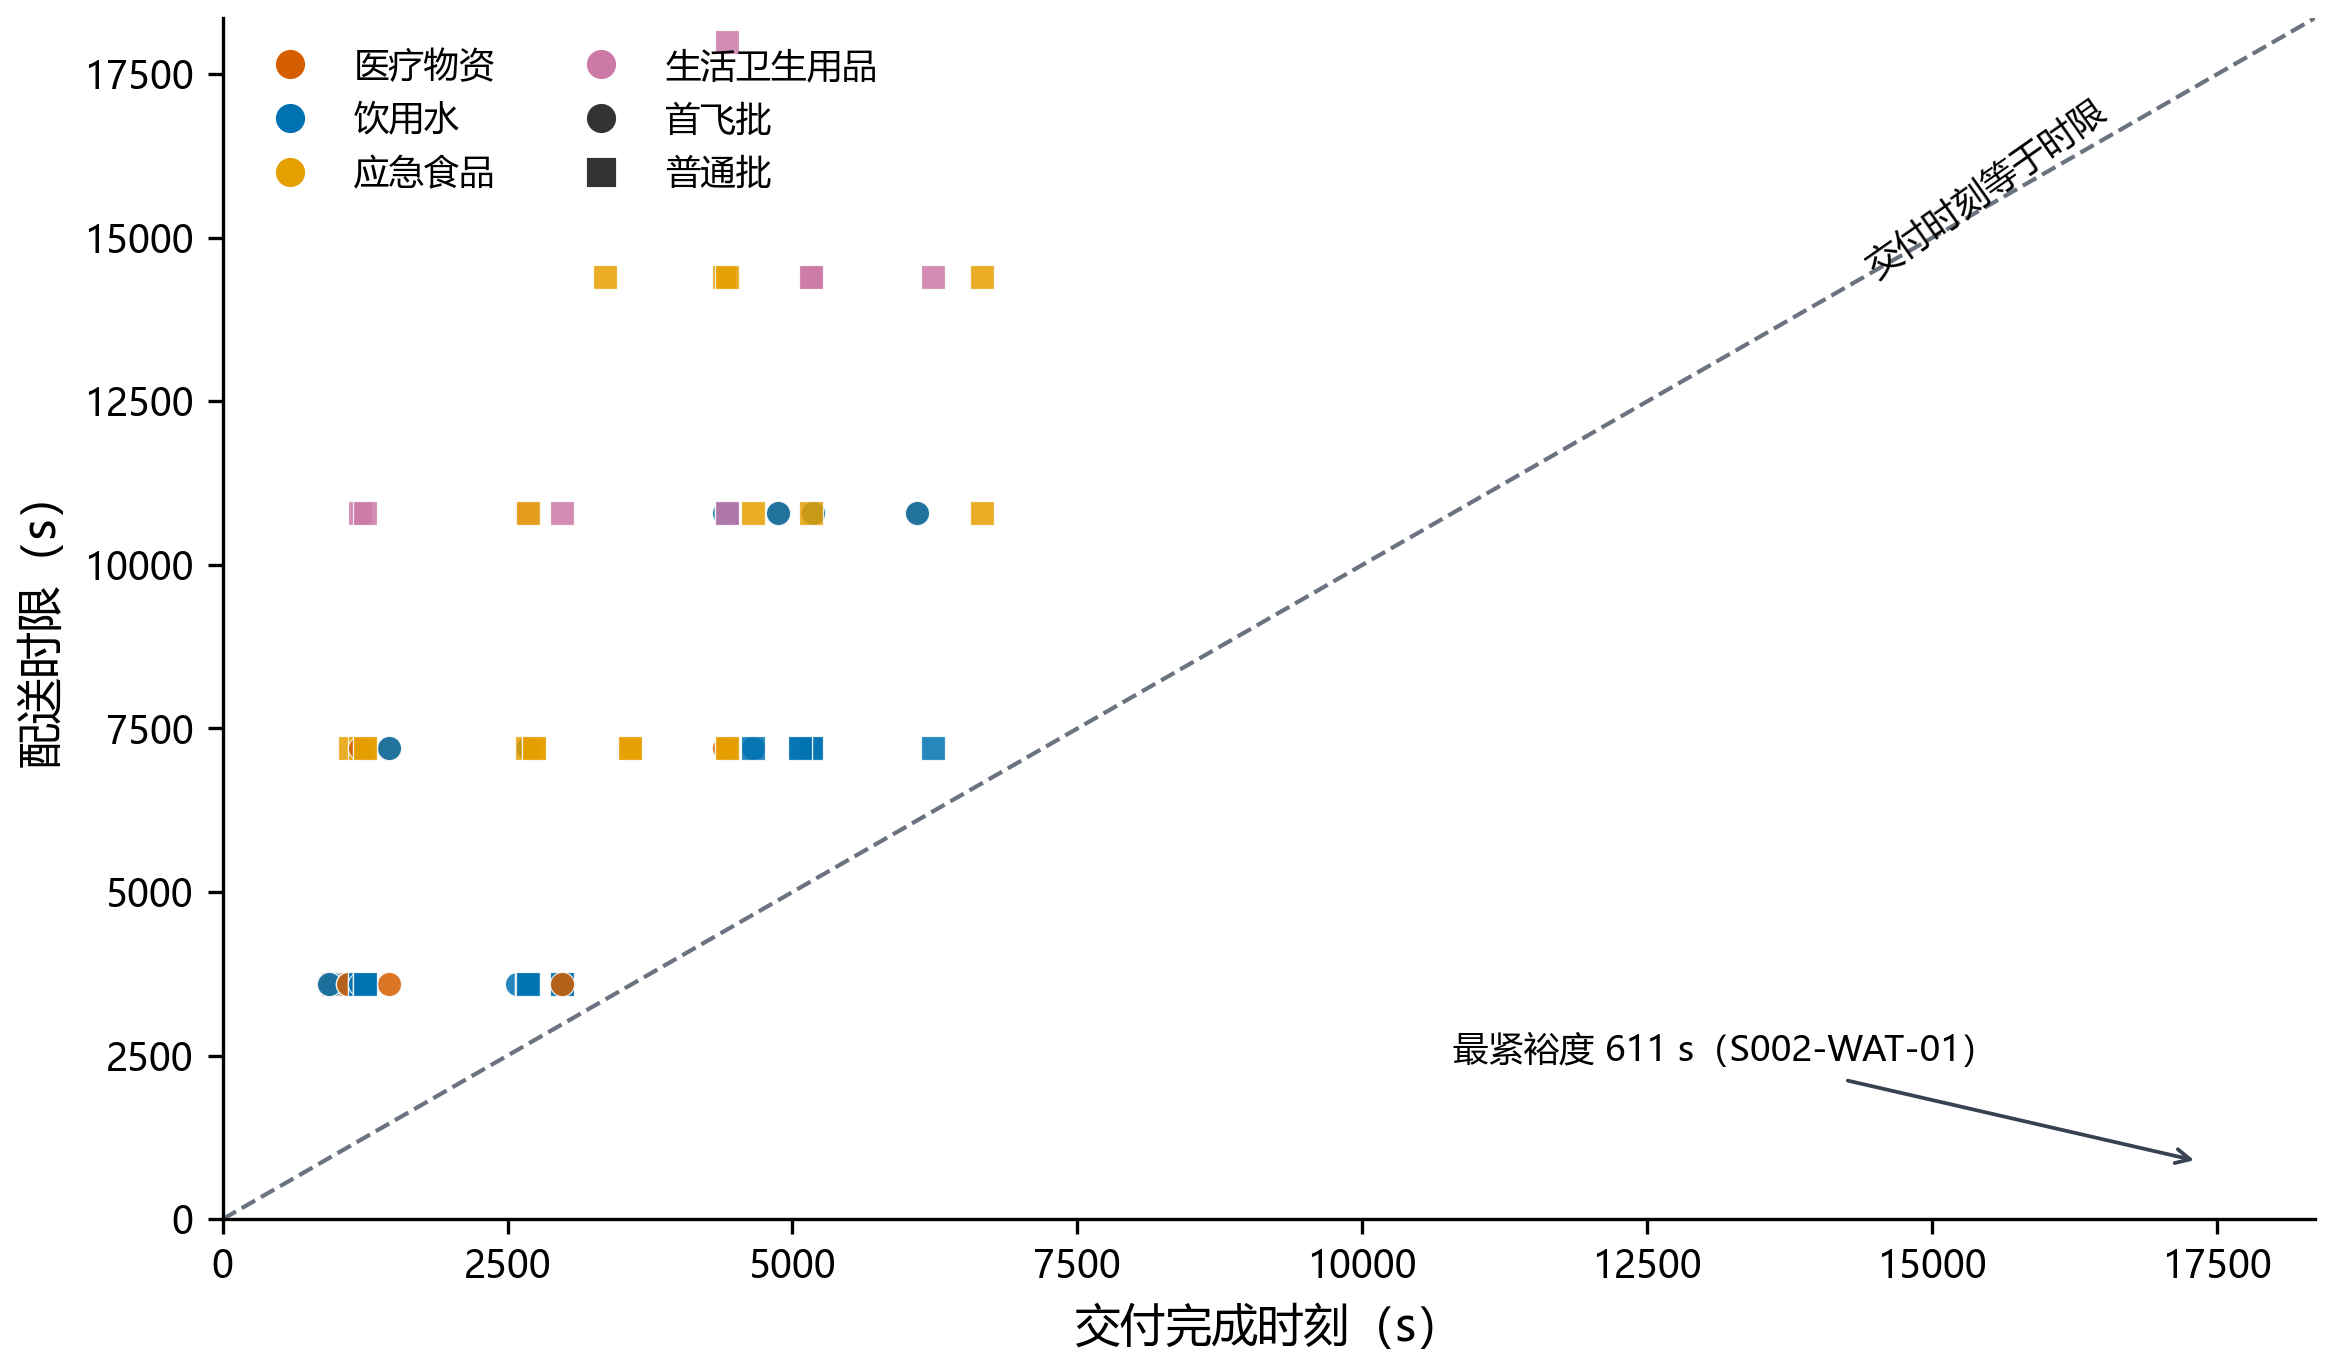
\includegraphics[width=0.86\textwidth]{figures/p2_delivery.png}
\caption{逐箱交付时刻与配送时限（圆点为首飞批，方块为普通批）}
\label{fig:delivery}
\end{figure}
\item \textbf{通信约束尚未计入}：本节的方案未考虑飞行全程通信，若按直连
判定，部分服务区作业段将被山体遮挡，需经中继保障，相关联合调度见第
\ref{sec:p3}节。
\end{enumerate}
% 问题三
\section{问题三：通信约束下运输与中继联合调度}
\label{sec:p3}

\subsection{问题分析}

第五节给出了纯运输调度方案，但未考虑通信约束。题目要求无人机整个飞行过程与
调度中心保持通信，可行方式为直连或经悬停中继的双跳。镇龙乡山高谷深，低空
作业段与穿越山谷的巡航段极易被山体遮挡，直连无法全程成立，需在合适位置布设
中继并安排其工作时段。因此问题三需要将运输调度与中继布设调度联合优化：
中继位置决定哪些时段必须中继，运输架次的时刻安排必须与中继服务窗口相容，
反之中继架次也要在能源预算内覆盖全部必要时段。

\subsection{通信链路模型}

\subsubsection{自由空间损耗与链路预算}

工作频率 $f=2400$\,MHz，收发间三维距离
$D=\sqrt{d_{\mathrm{2D}}^2+\Delta z^2}$，单位公里，自由空间损耗按式
\eqref{eq:fspl} 计算\cite{refITU}。

\begin{equation}
L_{\mathrm{FSPL}}=32.45+20\lg f_{\mathrm{MHz}}+20\lg D_{\mathrm{km}}
\label{eq:fspl}
\end{equation}

接收功率为发射功率减去自由空间损耗、系统损耗与遮挡损耗三项。通信有效需接收
功率不低于接收门限 $P_{\mathrm{th}}=P_{\mathrm{sens}}+M=-98+8=-90$\,dBm，
等价于链路总损耗不超过上限，即直连 122\,dB、经中继的接入链路 116\,dB、
中继到 O01 的回程链路 126\,dB。由式 \eqref{eq:fspl} 反解，三档上限对应的
最大三维距离约为 12.5、6.3、10.7\,km。

\subsubsection{地形遮挡判定}

对任意收发对，沿连线按 30\,m 步长采样，读取数字高程并与连线高度比较：任一
采样点地形高于连线则视距被遮挡，追加 10\,dB 遮挡损耗并判链路无效。无人机
位置沿其四维轨迹生成，即时间、经度、纬度、高度，故覆盖判定是确定性的。

\subsection{中继布设}

以覆盖采样法确定候选布设位置：对全部架次轨迹采样点先判直连有效，直接排除；
对直连失败点在若干地形高点候选位逐一检验接入链路与回程链路是否同时成立。
结果表明三个布设点即可覆盖全部需中继时段，其坐标如下。

\begin{itemize}
\item 西点 $P_W=(109.2103^{\circ}\mathrm{E},\,23.0471^{\circ}\mathrm{N},\,
676.5\,\mathrm{m})$：覆盖西与北片区，即 S001、S002、S003、S005、S007、
S008、S009、S011、S015 及其转运走廊；
\item 东点 $P_E=(109.2689^{\circ}\mathrm{E},\,23.0127^{\circ}\mathrm{N},\,
650.0\,\mathrm{m})$：覆盖东片区，即 S010、S012、S013、S014；
\item 北点 $P_N=(109.2343^{\circ}\mathrm{E},\,23.0592^{\circ}\mathrm{N},\,
600.0\,\mathrm{m})$：覆盖 S004 及经过其走廊的深入航线，因 S004 直连不可达
必须经中继。
\end{itemize}

三个布设点与服务区的地理聚类一致，即西与北九区、东四区、S004 独点，
为第\ref{sec:p4}节的分区提供了依据。图 \ref{fig:p3cov} 给出布设点与
6.3\,km 接入半径示意。

\begin{figure}[htbp]
\centering
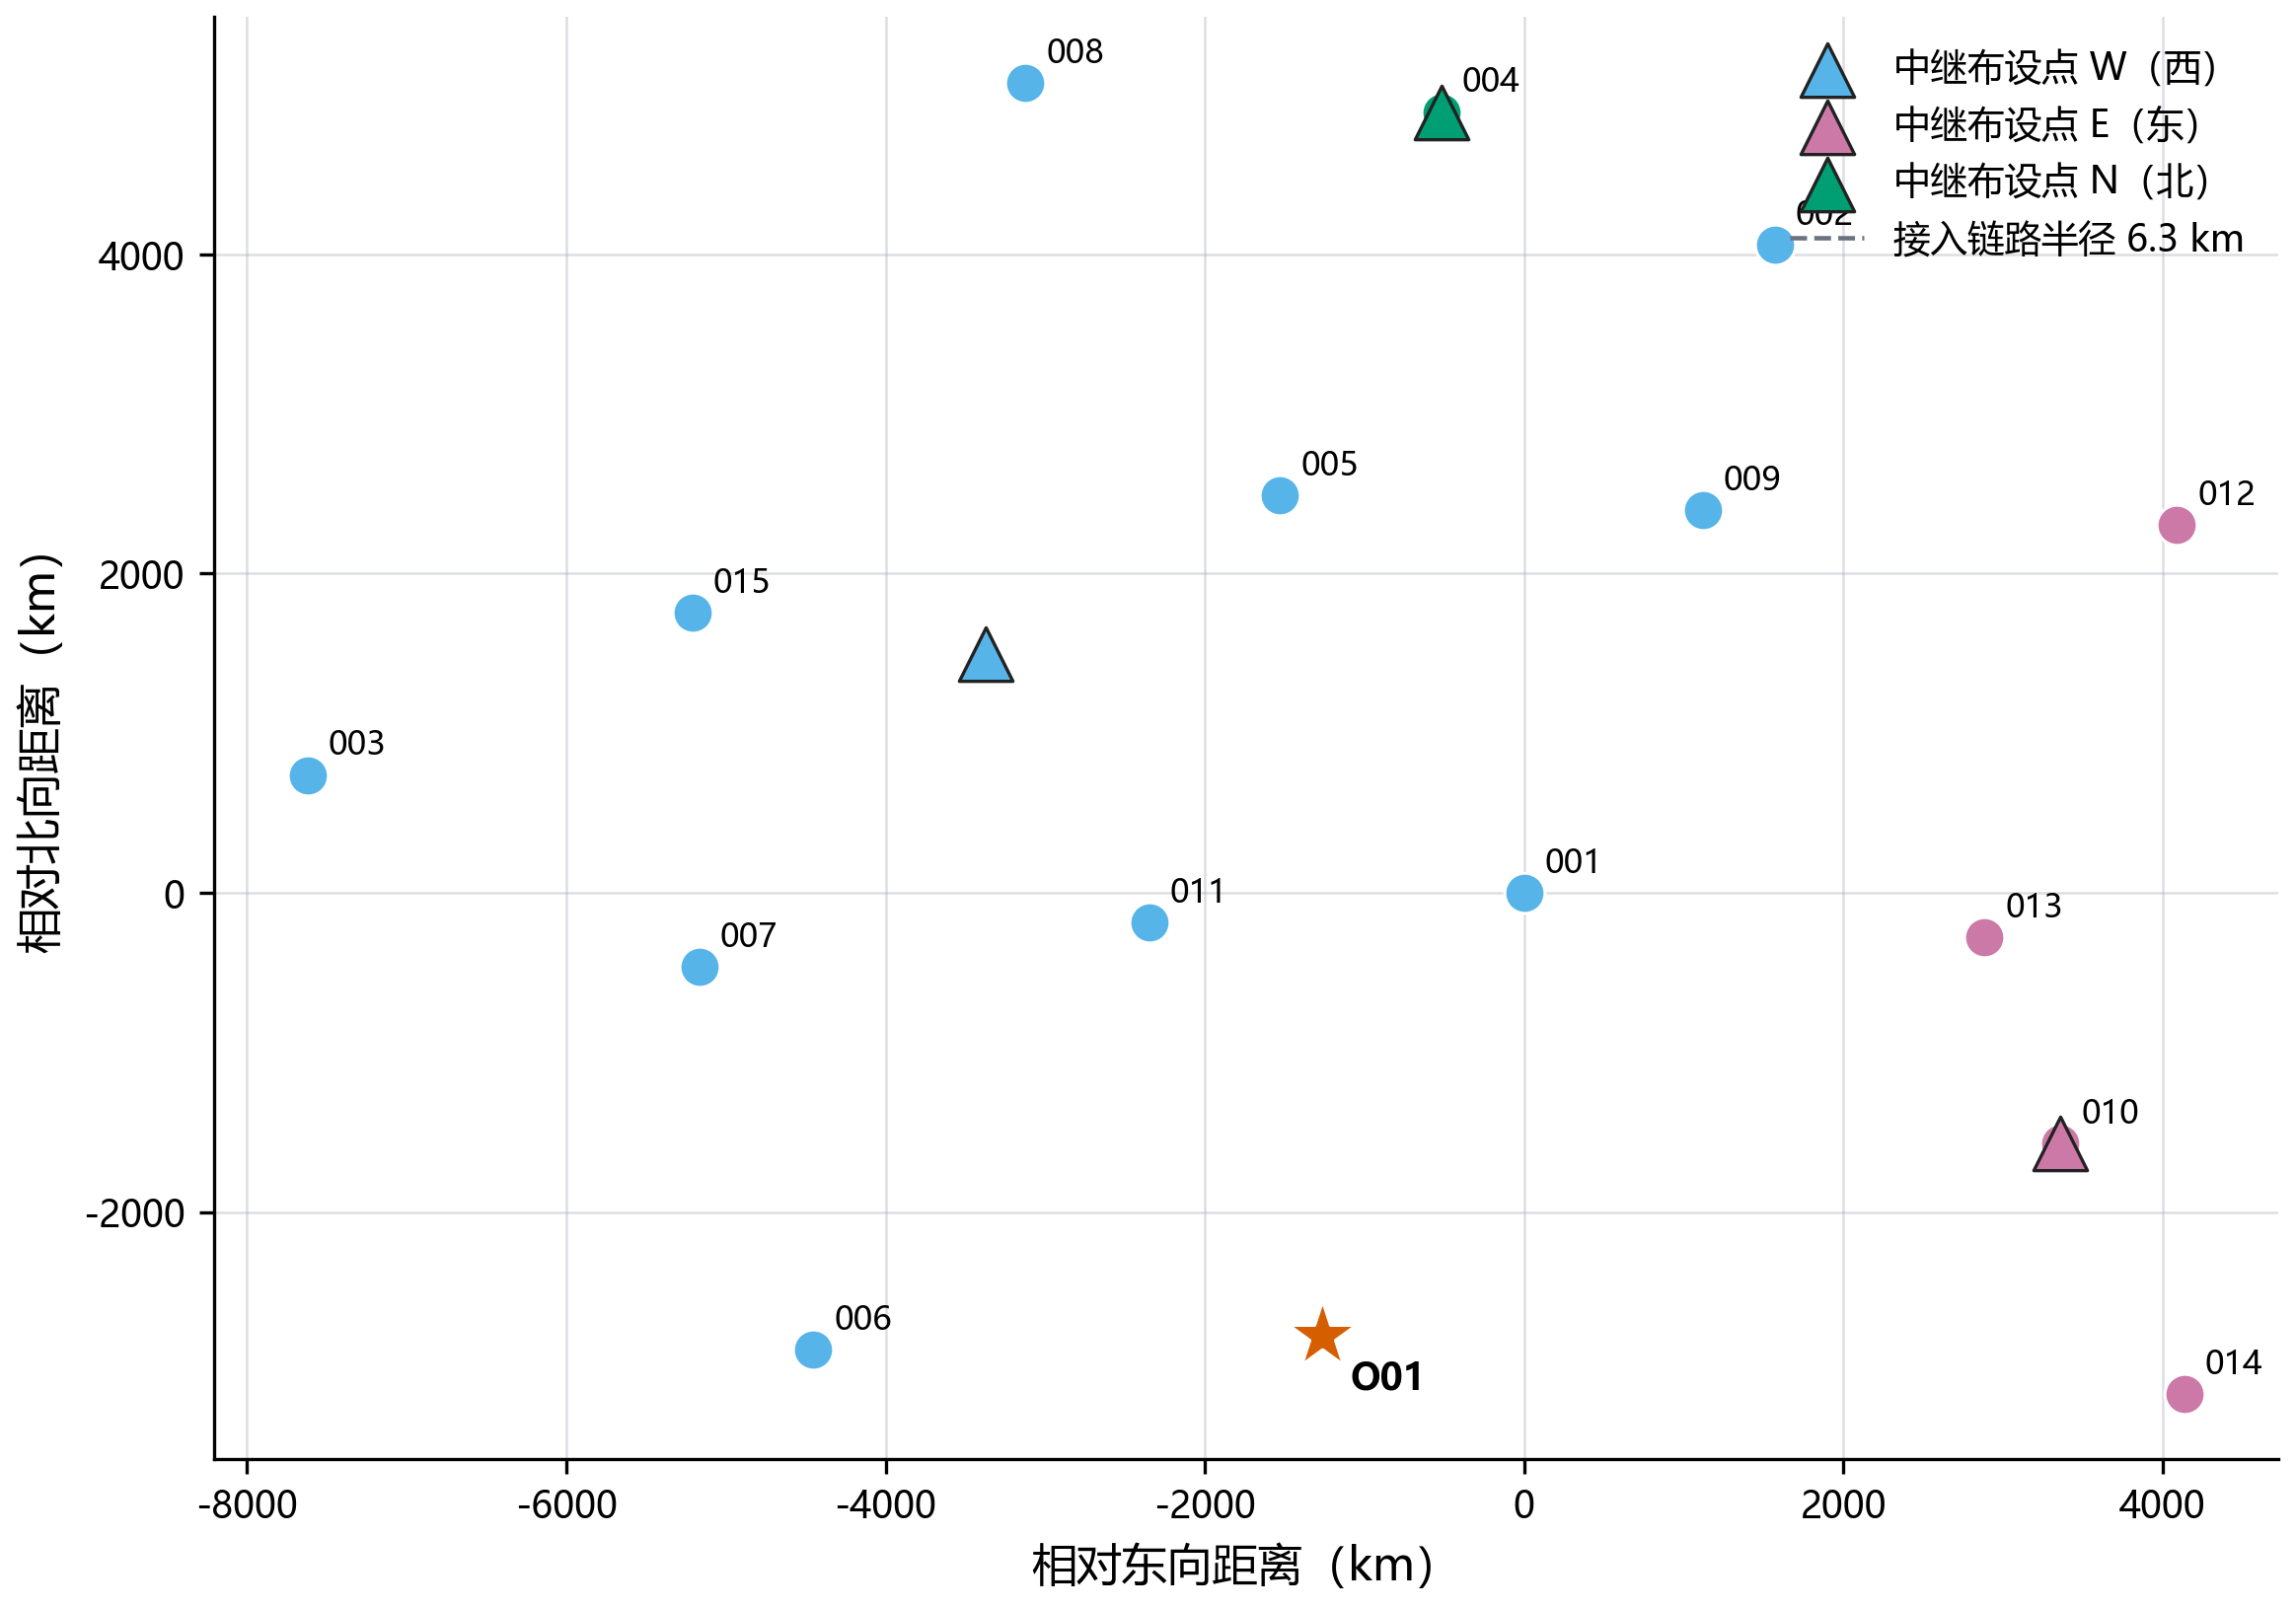
\includegraphics[width=0.76\textwidth]{figures/p3_coverage.png}
\caption{三个中继布设点及其接入链路半径示意（虚线圆半径 6.3 km）}
\label{fig:p3cov}
\end{figure}

\subsection{运输与中继的联合调度}

\subsubsection{逐区段通信判定}

对每个架次，沿轨迹对服务区作业段与相邻转运段逐点判定：直连有效者保持直连；
直连失败者分配给某一中继布设点，要求接入与回程链路同时满足，且该点当前处于
服务窗口。任一采样点无可用链路即记为盲区。覆盖判定对全部架次轨迹执行，得到
每个需中继的飞行阶段、其归属布设点与起止时刻，作为中继排班的输入。

\subsubsection{覆盖审核与中继时序规划}

对第五节选区的 28 架次区一致方案按 30\,m 步长做通信审核，得到 1762 个需中继采样点。
初始中继布设即实现全覆盖：西点、东点与北点三个布设点的接入与回程链路在全部采样点
均可行，初始方案未做人工调整。中继单架次能源预算为 $(1-\rho)E_{\mathrm{use}}=2.56$\,kWh，
三班均未超预算。

最终两架中继的时间分片方案如下：
\begin{itemize}
\item 中继 1 驻西点，服务时段 [1058, 7453]\,s，能耗 2.184\,kWh，返航荷电状态约
$1-2.184/3.2=31.8\%$，高于 20\% 的安全下限；
\item 中继 2 先驻东点，服务时段 [1060, 5498]\,s，能耗 1.549\,kWh；再返航换装满充组件并转场北点，
服务时段 [6565, 7308]\,s，能耗 0.488\,kWh；最后转场西点承担 W 尾段 [8605, 9072]\,s，
能耗 0.372\,kWh。三个时段窗口不重叠，转场衔接经严格口径核算仅有 58\,s 转场等待。
\end{itemize}

按题目附录 2 的严格口径复核：每次任务含 180\,s 起飞准备、30\,s
建链与 300\,s 架次周转；能源组件复用前必须充满（初始 SOC 为 100\%，用后按
两阶段曲线充至 100\%）。东点班返航荷电约 $1-1.549/3.2=51.6\%$，北点班取自
6 组件共享池内的满充新组件，不受东点班组件充电进度约束；北点班派单 6100\,s
与东点班返场 5857\,s 间隔 243\,s，西点尾段班派单 8182\,s 与北点班返场 7763\,s
间隔 419\,s，经组件池就绪时间核算仅产生 58\,s 的转场
等待（machine\_pen$=58$\,s），不影响各窗口中继覆盖。西点需求总时长约 8014\,s，
单班服务能耗将超过 2.56\,kWh 的能源预算，故拆为 W1 与 W2 两班，间隙 1152\,s
用于中继转场与组件轮换。中继最晚返场为西点尾段班 9491\,s，晚于运输侧偏移后
完工约 9473\,s，故联合任务完工时间由中继 1 尾段班返场决定，
为 9491\,s（约 158.2\,min）。

需中继采样点按布设点归属的空间分布见图 \ref{fig:relaycover}：西片区与北部
走廊归西点、东片区归东点、S004 走廊归北点，三组聚类清晰、无重叠，构成问题四
任务分区的地理基础。

\begin{figure}[htbp]
\centering
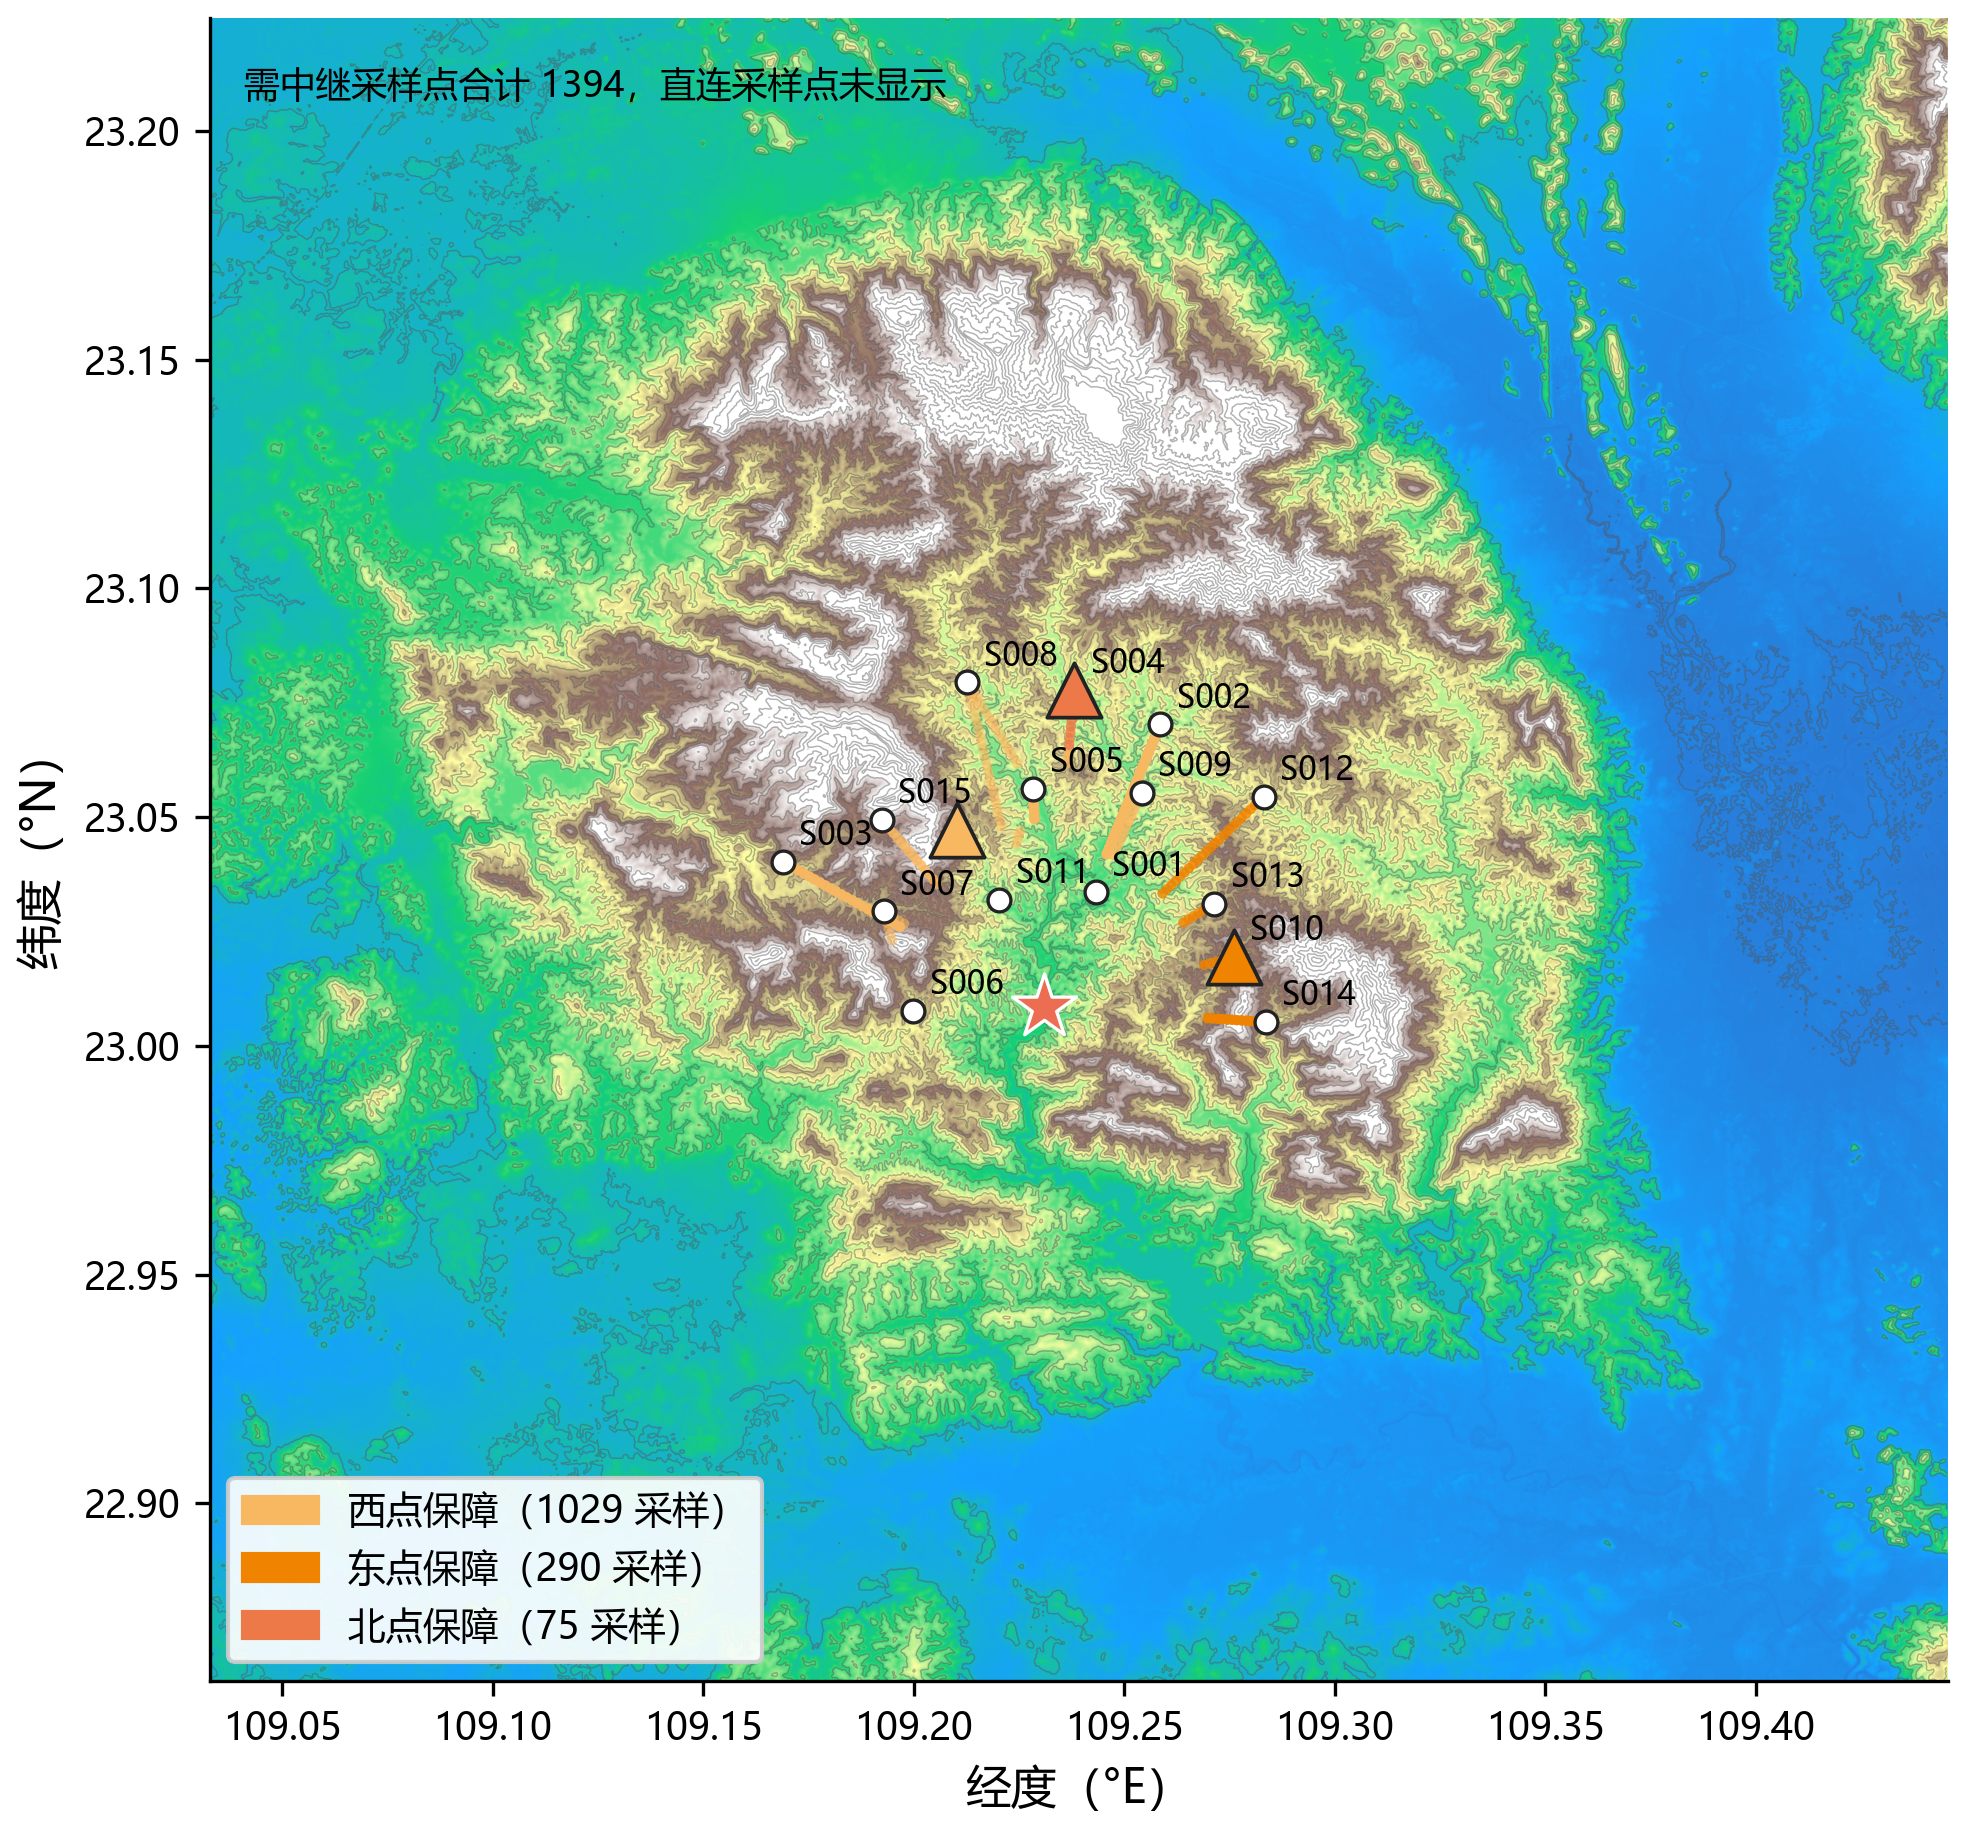
\includegraphics[width=0.96\textwidth]{figures/p3_relay_coverage.png}
\caption{1762 个需中继采样点按布设点的归属分布（DEM 底图）}
\label{fig:relaycover}
\end{figure}

中继架次明细见表 \ref{tab:relay}，图 \ref{fig:relaytl} 给出两架中继四个服务时段的时间线。

\begin{figure}[htbp]
\centering
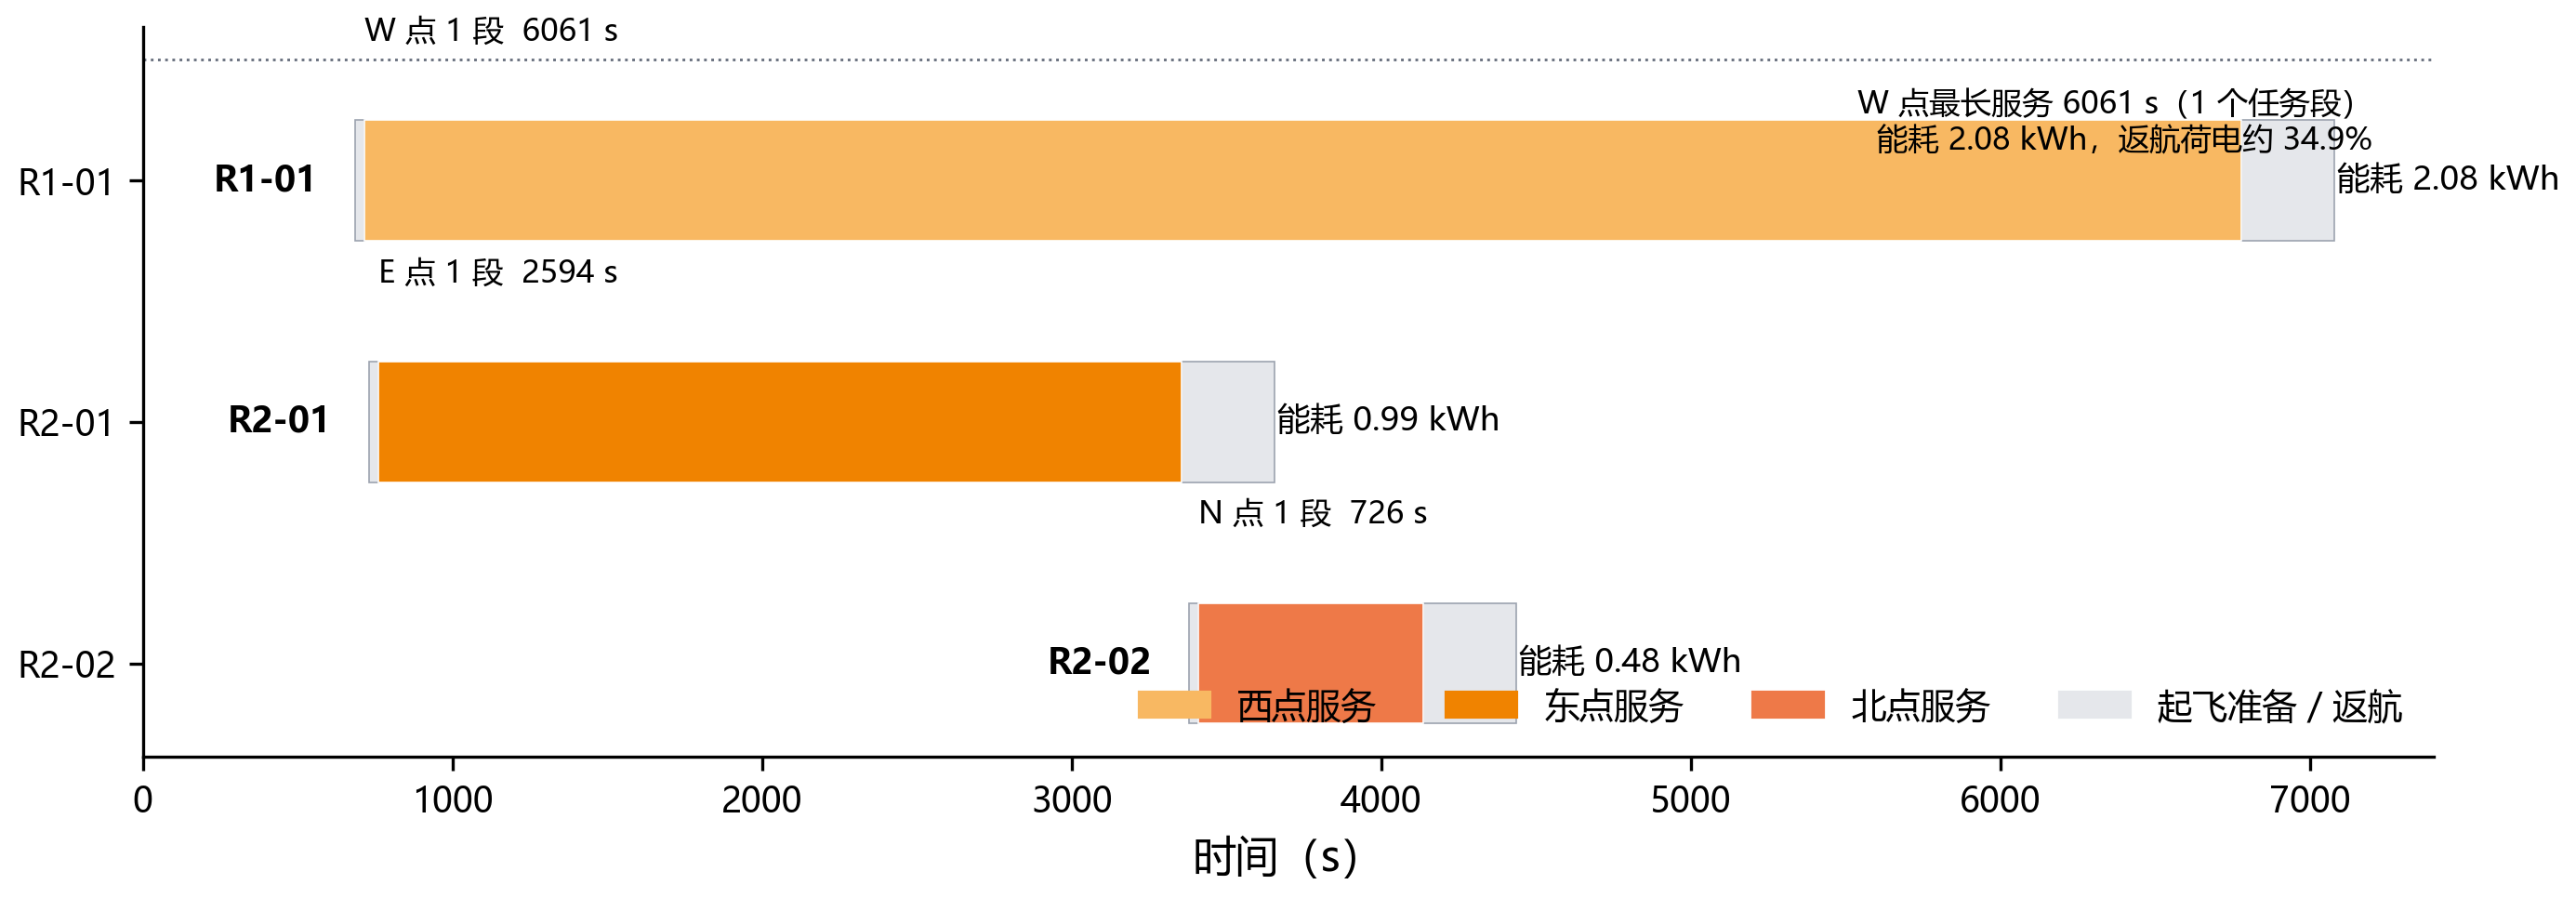
\includegraphics[width=0.98\textwidth]{figures/p3_relay_tl.png}
\caption{两架中继四个服务时段的时间线（浅灰为起飞准备与返航）}
\label{fig:relaytl}
\end{figure}

\begin{table}[htbp]
\centering
\caption{中继架次安排（中继 1 驻西点，中继 2 依次东点、北点、西点尾段）}
\label{tab:relay}
\begin{tabular}{ccccccc}
\toprule
中继架次 & 无人机 & 能源组件 & 任务位置 & 服务时段(s) & 能耗(kWh) & 覆盖状态 \\
\midrule
R1-01 & 中继1 & 组件1 & 西点 & [1058, 7453] & 2.184 & 全覆盖 \\
R1-02 & 中继1 & 组件2 & 西点 & [8605, 9072] & 0.372 & 全覆盖 \\
R2-01 & 中继2 & 组件3 & 东点 & [1060, 5498] & 1.549 & 全覆盖 \\
R2-02 & 中继2 & 组件4 & 北点 & [6565, 7308] & 0.488 & 全覆盖 \\
\bottomrule
\end{tabular}
\end{table}

\subsection{联合调度结果}

协同后的运输方案仍为 28 架次区一致方案（与第五节一致），全部货箱按时投送至
各自指定服务区（三档时限零违反、加权迟到为零）。通信方面，
西点两班与东、北两班中继分别承担 2.184、0.372、1.549 与 0.488\,kWh，
中继合计约 4.59\,kWh；
自动化覆盖诊断确认初始布设即全覆盖（1762 个需中继采样点零未覆盖），
中继四班均满足能源预算，东转北衔接经组件池严格口径核算仅 58\,s 转场等待。为
对齐中继时窗，对需北点覆盖的 S004 所属架次施加后移偏移（f22 约 2100\,s），
带动相关链小幅顺延，偏移后运输完工约 9473\,s；中继 1 西点尾段班最晚返场
9491\,s 决定联合完工——中继约束引入的
完工代价约 2096\,s（较纯运输 7395\,s，约 28.3\%），集中于北点窗口与西点长班
覆盖的必要等待。
表 \ref{tab:p3cmp} 给出与纯运输方案的指标对比，图 \ref{fig:p3gantt}
给出运输与中继的联合甘特图。图 \ref{fig:commtl} 给出每个运输架次的通信
保障方式时间线，浅灰段为直连，彩色段为中继，可见需中继的时段集中于西与北
片区作业段与 S004 走廊，且全部落在对应中继的服务窗口内；架次明细见表
\ref{tab:p3flights}。

\begin{figure}[htbp]
\centering
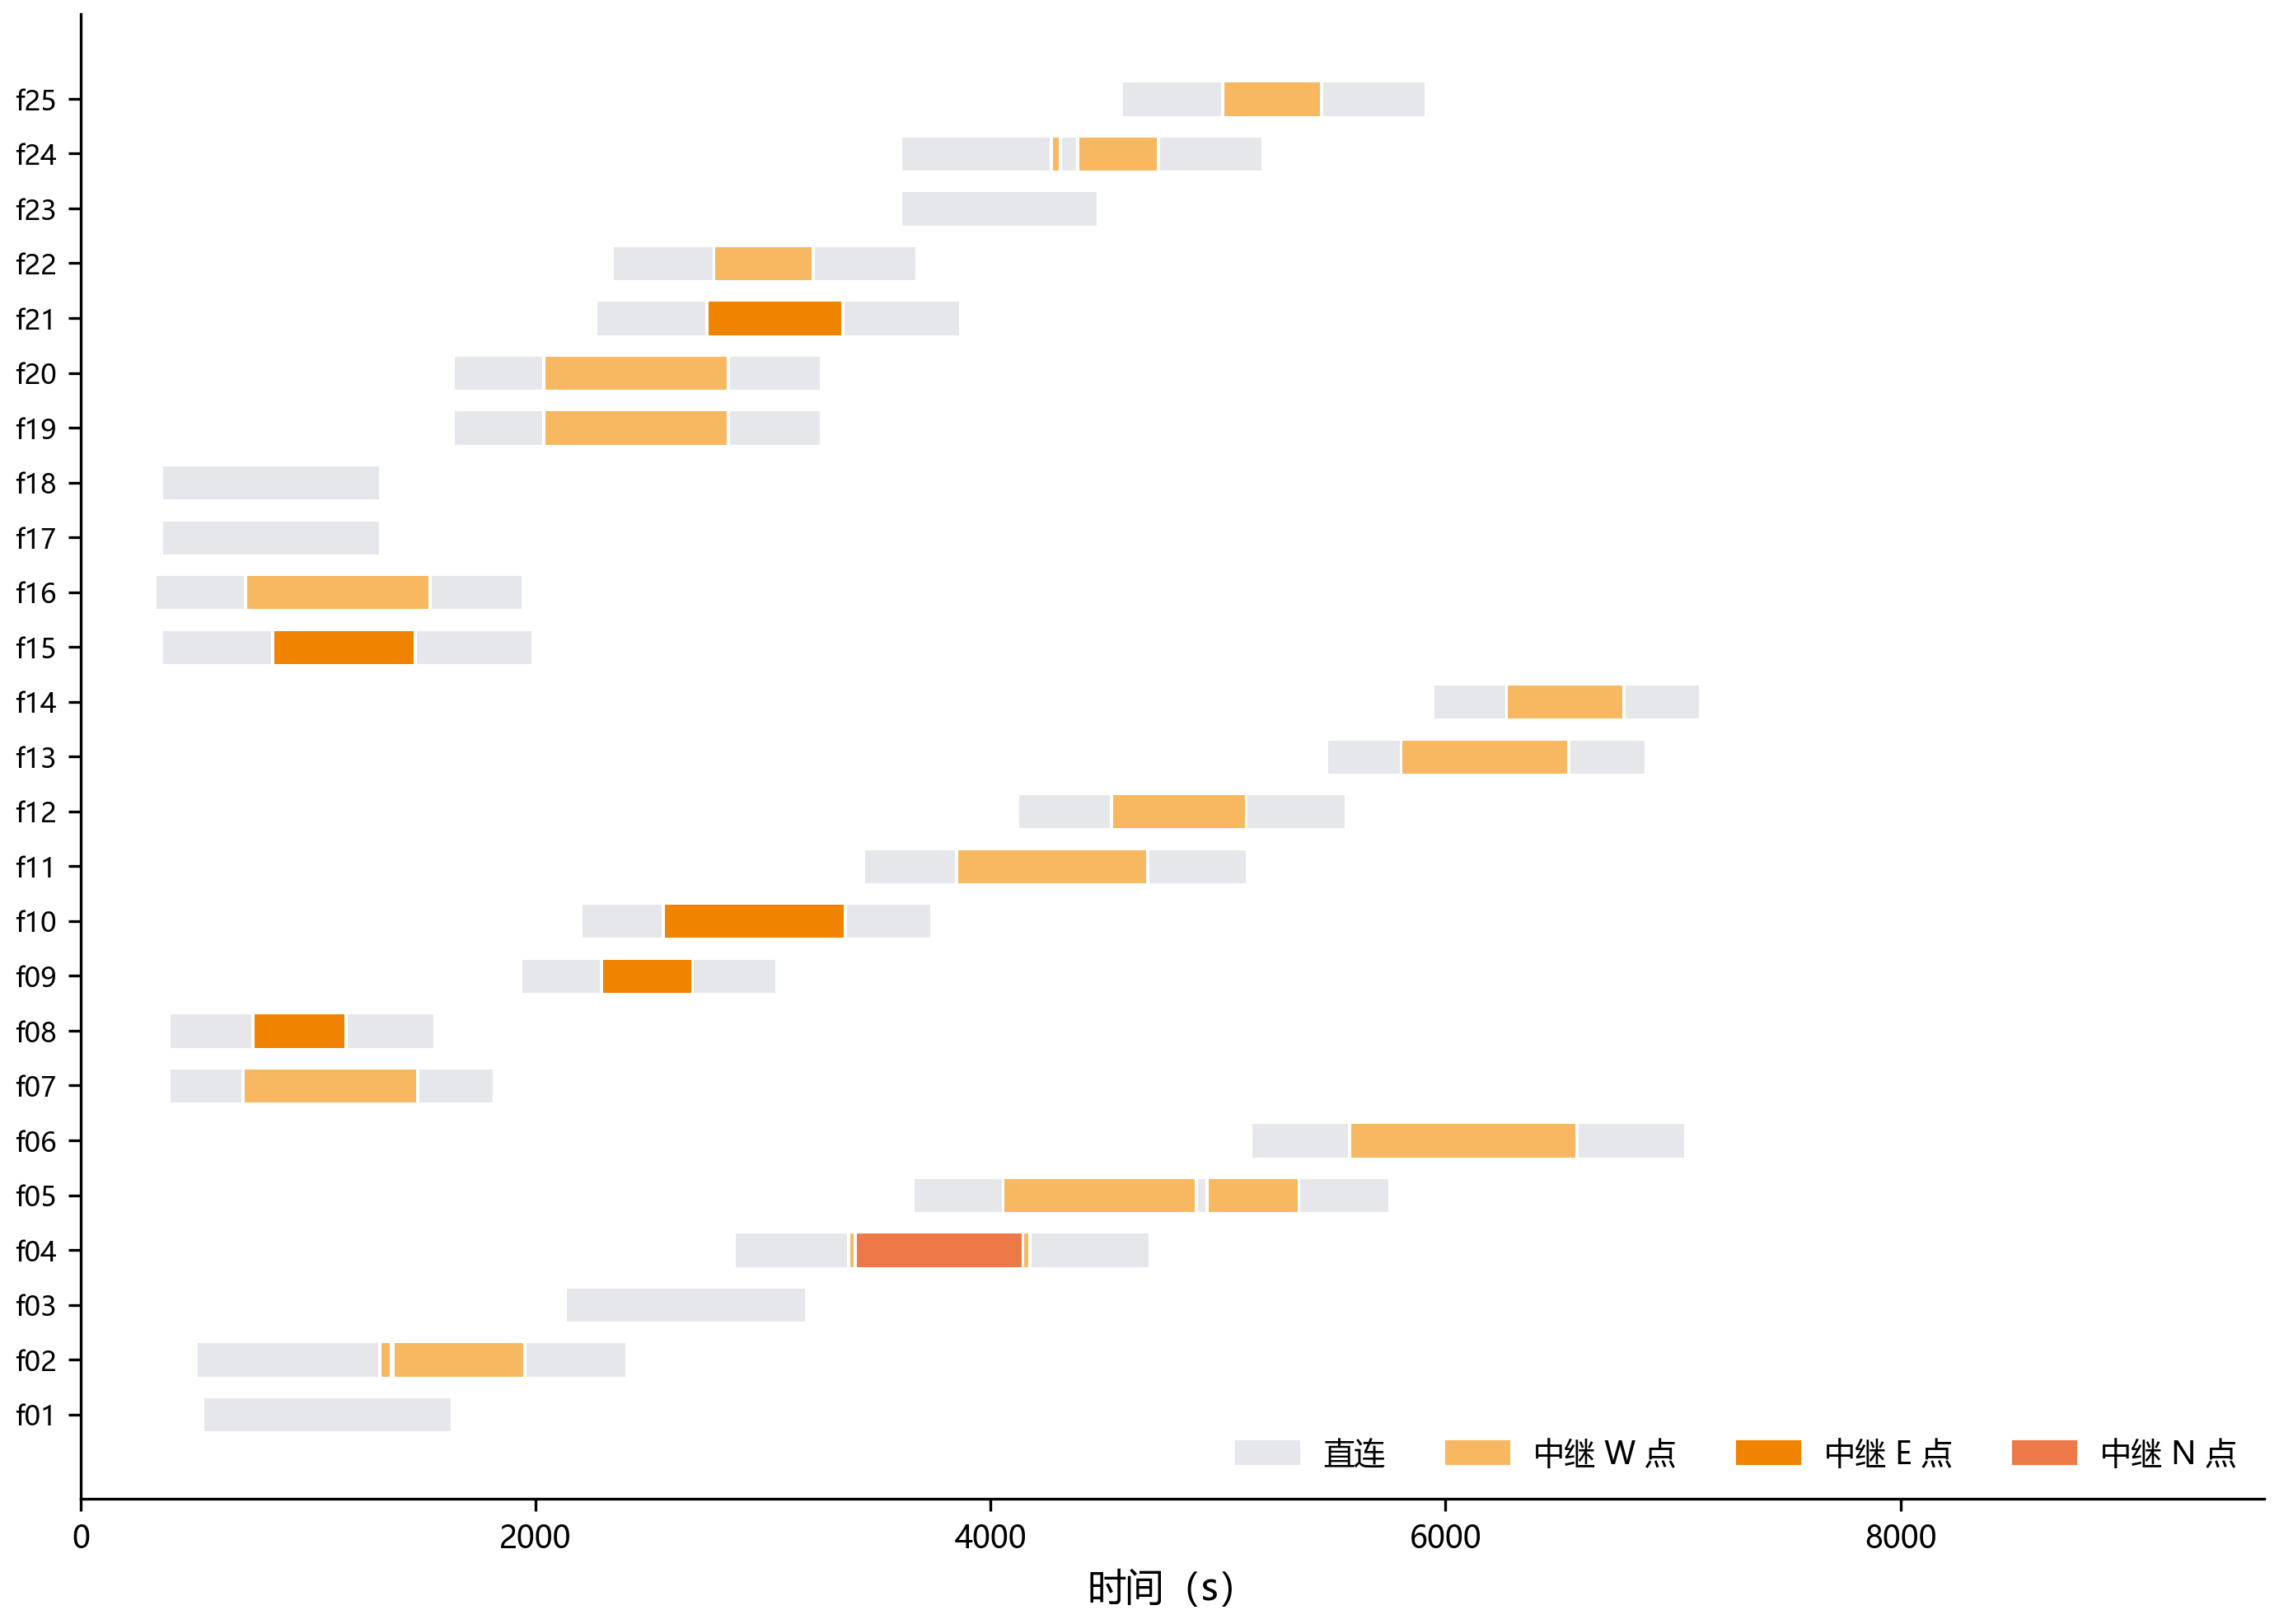
\includegraphics[width=0.98\textwidth]{figures/p3_comm_tl.png}
\caption{各运输架次的通信保障方式时间线（浅灰为直连，彩色为中继）}
\label{fig:commtl}
\end{figure}

\begin{table}[htbp]
\centering
\caption{问题三协同方案主要指标（与问题二对比）}
\label{tab:p3cmp}
\begin{tabular}{lccc}
\toprule
指标 & 问题二（纯运输） & 问题三（协同） & 变化 \\
\midrule
架次数 & 28 & 28 & 不变 \\
完工时间(s) & 7395 & 9491 & 中继尾段班返场 +2096（28.3\%） \\
运输能耗(kWh) & 83.12 & 83.12 & 不变 \\
中继能耗(kWh) & 未计 & 4.59 & 四班保障 \\
通信盲区 & 未计 & 0 & 初始布设即全覆盖 \\
中继架次 & 无 & 4 时段 & 两架分片复用 \\
\bottomrule
\end{tabular}
\end{table}

\begin{figure}[htbp]
\centering
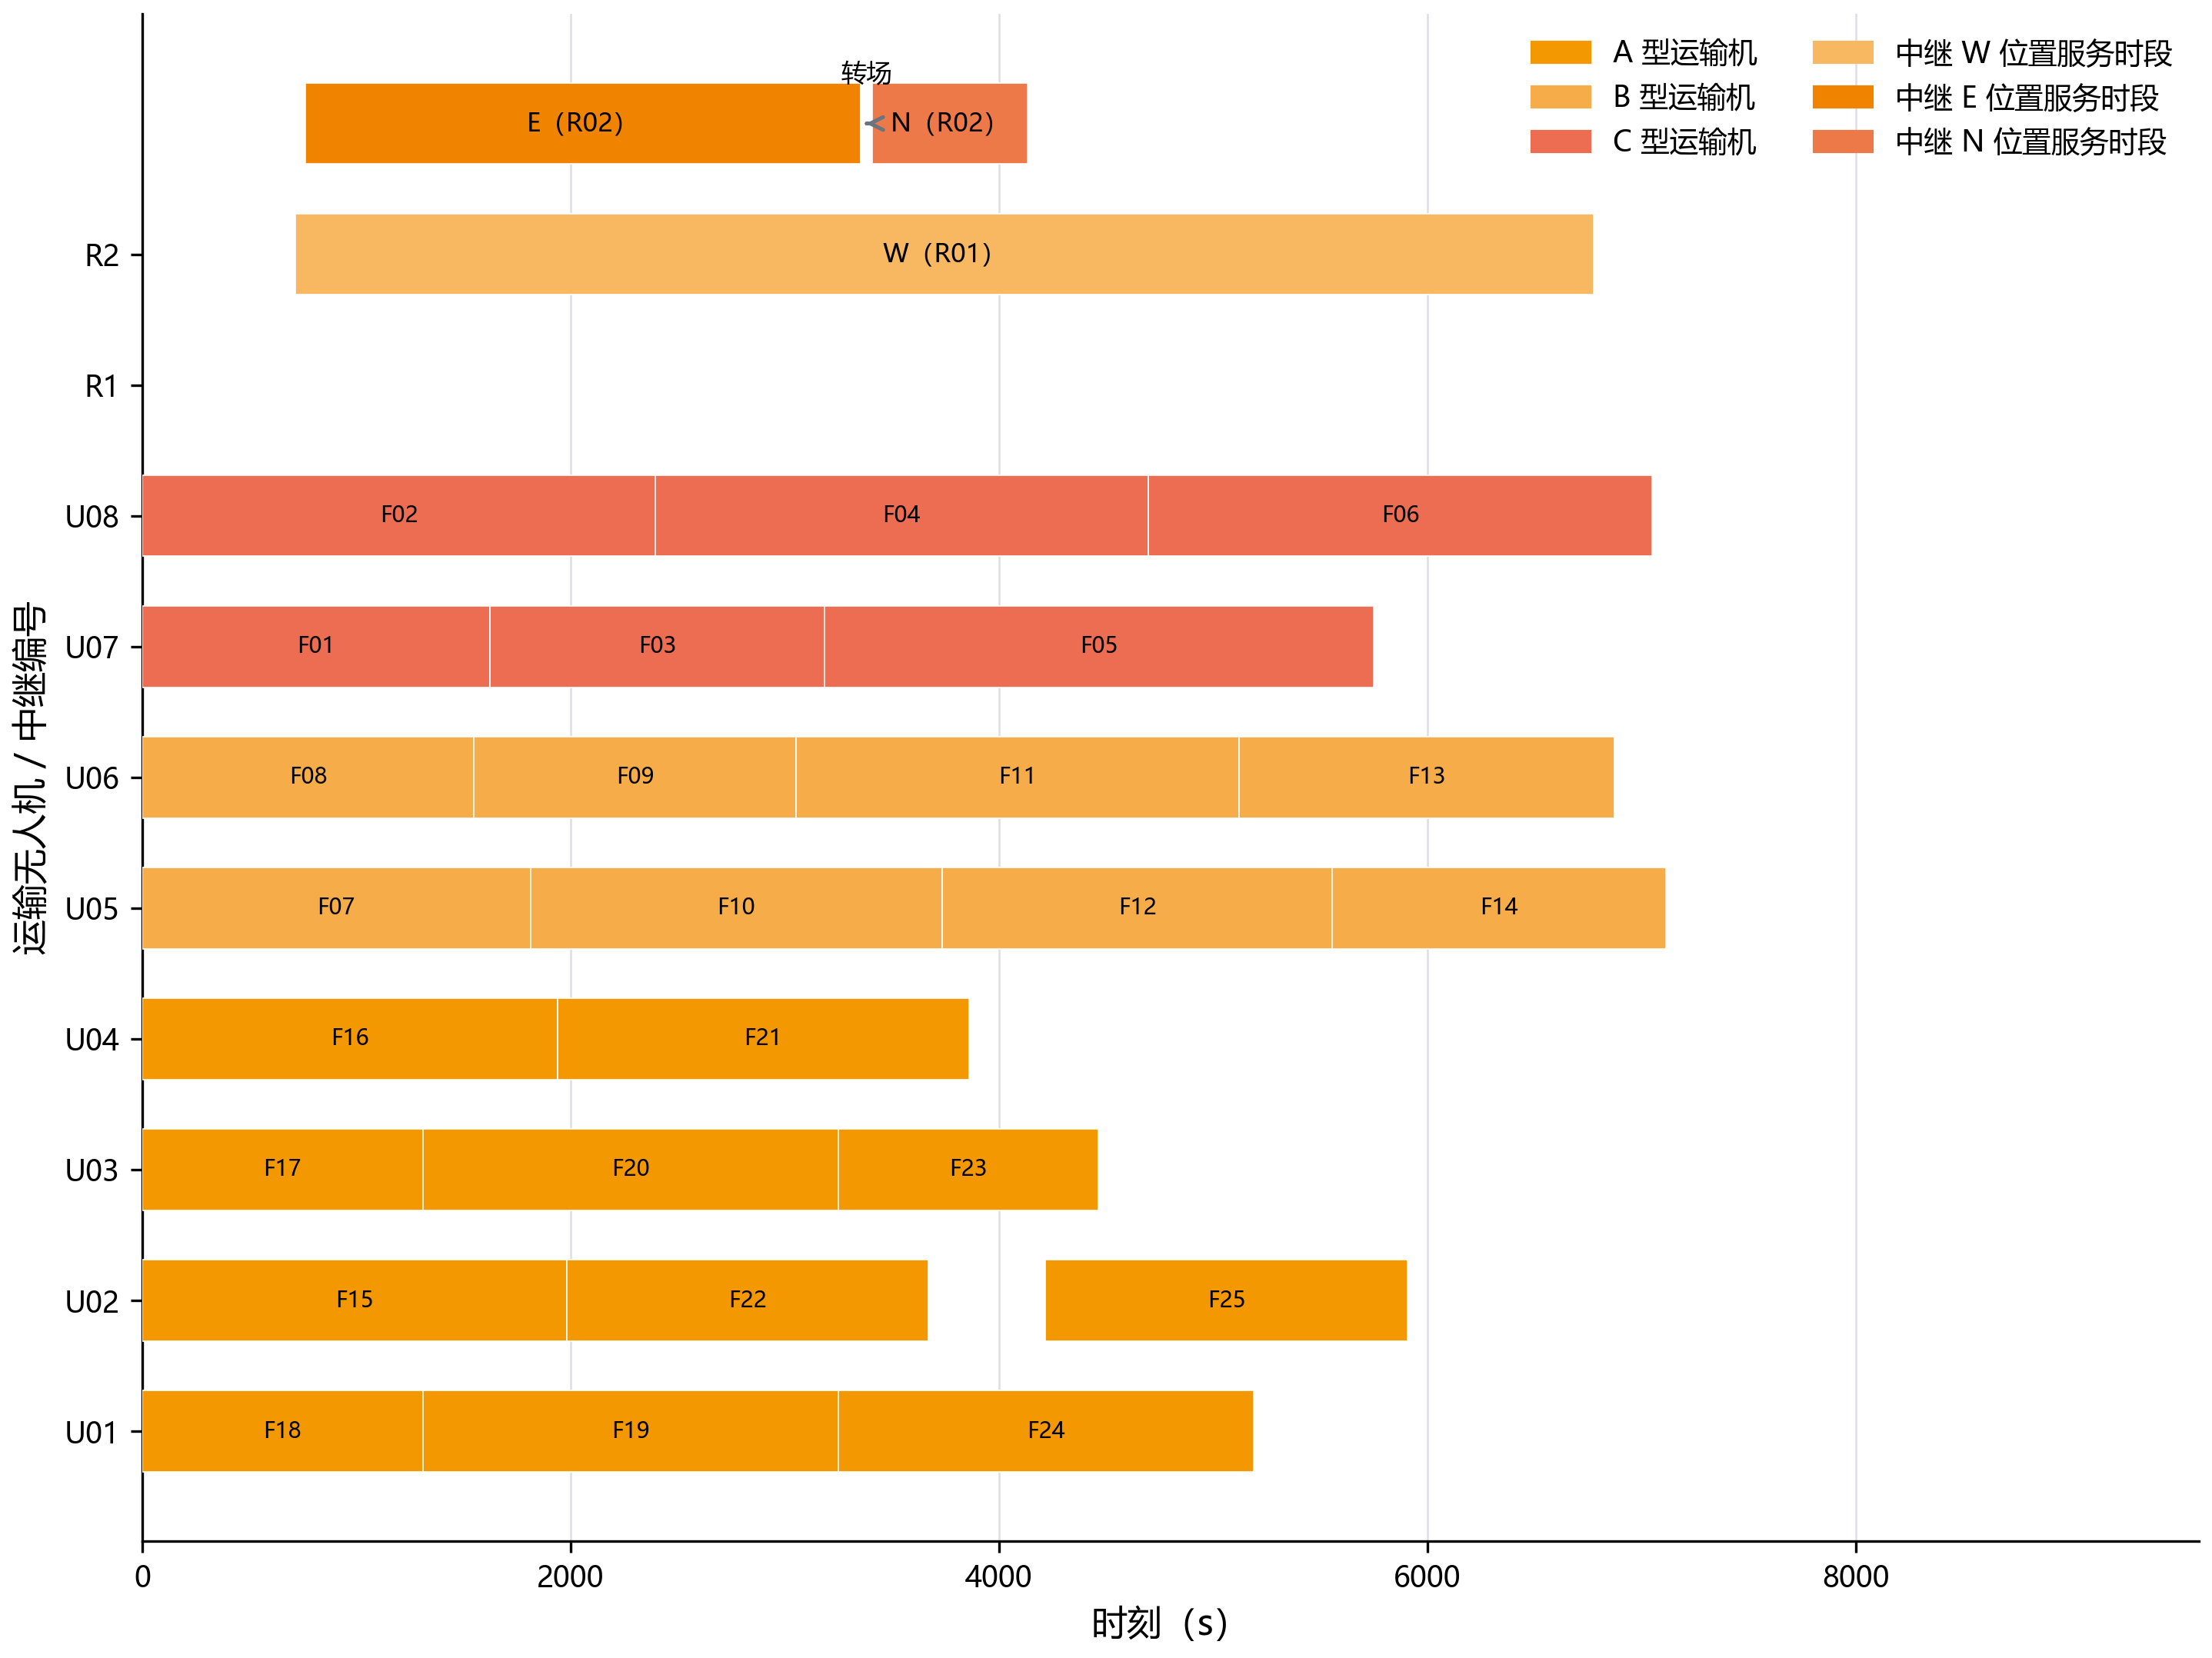
\includegraphics[width=0.98\textwidth]{figures/p3_gantt.png}
\caption{运输与中继协同调度甘特图（上：8 架运输机；下：中继 1 与中继 2 时段）}
\label{fig:p3gantt}
\end{figure}

\begin{table}[htbp]
\centering
\caption{问题三协同方案架次明细（28 架次，时刻为对齐中继窗口后的偏移派单）}
\label{tab:p3flights}
\small
\begin{tabular}{ccccccc}
\toprule
架次 & 机型 & 无人机 & 开始(s) & 返回(s) & 能耗(kWh) & 航线 \\
\midrule
f16 & C & U07 & 300 & 1858 & 2.99 & S001 \\
f24 & C & U08 & 300 & 1791 & 2.36 & S006 \\
f17 & C & U08 & 1791 & 3218 & 2.40 & S001 \\
f18 & C & U07 & 1858 & 3895 & 5.71 & S002 \\
f03 & C & U08 & 3218 & 5639 & 5.89 & S003 \\
f26 & C & U08 & 5639 & 7694 & 5.39 & S008 \\
f22 & C & U07 & 5700 & 7867 & 5.51 & S004 \\
f23 & C & U08 & 7863 & 9473 & 3.46 & S005 \\
\midrule
f10 & B & U05 & 300 & 2407 & 2.27 & S010至S014 \\
f25 & B & U06 & 300 & 1921 & 1.77 & S007 \\
f12 & B & U06 & 1921 & 3842 & 2.75 & S012 \\
f07 & B & U05 & 2407 & 4433 & 2.15 & S007至S015 \\
f09 & B & U06 & 3842 & 5866 & 2.79 & S002至S009 \\
f11 & B & U05 & 4433 & 6346 & 2.46 & S013至S011 \\
f05 & B & U06 & 5866 & 7302 & 1.74 & S009 \\
f29 & B & U05 & 6346 & 7408 & 0.89 & S011 \\
\midrule
f01 & A & U01 & 300 & 1609 & 1.26 & S001 \\
f14 & A & U03 & 300 & 2281 & 2.29 & S014 \\
f36 & A & U02 & 300 & 1906 & 1.95 & S013 \\
f39 & A & U04 & 300 & 2728 & 3.28 & S002至S005 \\
f02 & A & U01 & 1609 & 4038 & 3.22 & S002至S005 \\
f06 & A & U02 & 1906 & 4270 & 2.85 & S006至S015 \\
f08 & A & U04 & 2728 & 4889 & 3.19 & S008 \\
f21 & A & U01 & 4038 & 6288 & 3.08 & S003 \\
f28 & A & U02 & 4270 & 6755 & 3.40 & S010至S005 \\
f15 & A & U04 & 5109 & 7606 & 3.17 & S015至S005 \\
f04 & A & U03 & 5581 & 7758 & 3.08 & S004 \\
f37 & A & U01 & 6288 & 7940 & 1.80 & S007 \\
\bottomrule
\end{tabular}
\end{table}

\subsection{结果分析}

\begin{enumerate}
\item \textbf{通信保障以可核验的完工代价换取全程无盲区}：为对齐中继时窗，
S004 所属架次后移约 2100\,s 并带动相关链顺延，运输完工由纯运输的 7395\,s 变为
偏移后约 9473\,s；中继 1 西点尾段班返场 9491\,s 成为联合完工口径，较运输再增约
18\,s。中继约束引入的完工代价约 2096\,s（28.3\%），集中于北点窗口必须覆盖的
S004 走廊与西点长班保障；运输能耗 83.12\,kWh 与问题二持平，中继四班新增能耗
约 4.59\,kWh。代价可进一步由运输层面向中继窗口的联合排程压缩（见第
\ref{sec:sens}节讨论），但零盲区与零迟到在严格口径下始终成立。
\item \textbf{两架中继即可全程保障}：中继 1 驻西点，中继 2 先东、后北、再西点尾段的
分片复用，使四个服务时段由两架中继在时间上错峰满足。28 架次将任务分散为
更多短架次，中继窗口随之缩短：西点两班 2.184 与 0.372\,kWh、东点 1.549\,kWh、
北点 0.488\,kWh，合计较任务集中为少数长班次的对照排班方式显著下降。
\item \textbf{能源预算自洽}：西点需求总时长约 8014\,s，单班服务能耗将超过
2.56\,kWh 预算，故拆为 W1（106.6\,min 连续服务、能耗 2.184\,kWh、返航荷电
31.8\%）与 W2（能耗 0.372\,kWh）两班，班间间隙 1152\,s 供中继返场与组件轮换，
6 组能源组件足以支持；东点、北点单班能耗分别 1.549 与 0.488\,kWh，返航荷电
51.6\% 与 84.8\%，余量充足。
\item \textbf{S004 的独特地位}：S004 直连与东西两点均无法覆盖，必须由北点
中继（[6565, 7308]\,s 服务窗口，全部对应 S004 走廊），其余运输任务都不会
进入北点窗口，因此北点时段为 S004 专属；这同时决定了第\ref{sec:p4}节中
S004 独立成组的必要性。
\end{enumerate}
% 敏感性分析
\section{敏感性分析}
\label{sec:sens}

围绕模型的关键参数做系统性扰动，检验结论的结构稳定性。各项数值均来自对
最新求解产物的重算。

\subsection{返航安全余量比例的敏感性}

安全余量比例 $\rho$ 直接决定单架次可用能量，进而决定最大安全载荷、架次数与
总能耗。扫描结果如表 \ref{tab:rho} 所示，图 \ref{fig:rho} 给出架次与能耗的
变化曲线。$\rho$ 在 0.1 至 0.2 区间内架次与能耗不变，均为 18 架次、59.02\,kWh，
说明 20\% 的安全余量下效率尚有富余；$\rho$ 增至 0.25、0.30、0.35 时远区
C 型架次被逐步拆分，架次增至 19、20、25，能耗升至 60.96、67.10、77.63\,kWh，
安全换效率的代价加速显现；$\rho$ 由 0.35 增至 0.40 时架次数不变而能耗由
77.63 降至 74.62\,kWh，源于机型结构切换，即部分 C 型远区任务改由更经济的
组合完成。该曲线为应急指挥在安全与效率之间的权衡提供了直接依据。

\begin{table}[htbp]
\centering
\caption{返航安全余量比例对问题一方案的影响}
\label{tab:rho}
\begin{tabular}{lccccccc}
\toprule
$\rho$ & 0.10 & 0.15 & \textbf{0.20} & 0.25 & 0.30 & 0.35 & 0.40 \\
\midrule
架次数 & 18 & 18 & \textbf{18} & 19 & 20 & 25 & 25 \\
总能耗(kWh) & 59.02 & 59.02 & \textbf{59.02} & 60.96 & 67.10 & 77.63 & 74.62 \\
\bottomrule
\end{tabular}
\end{table}

\begin{figure}[htbp]
\centering
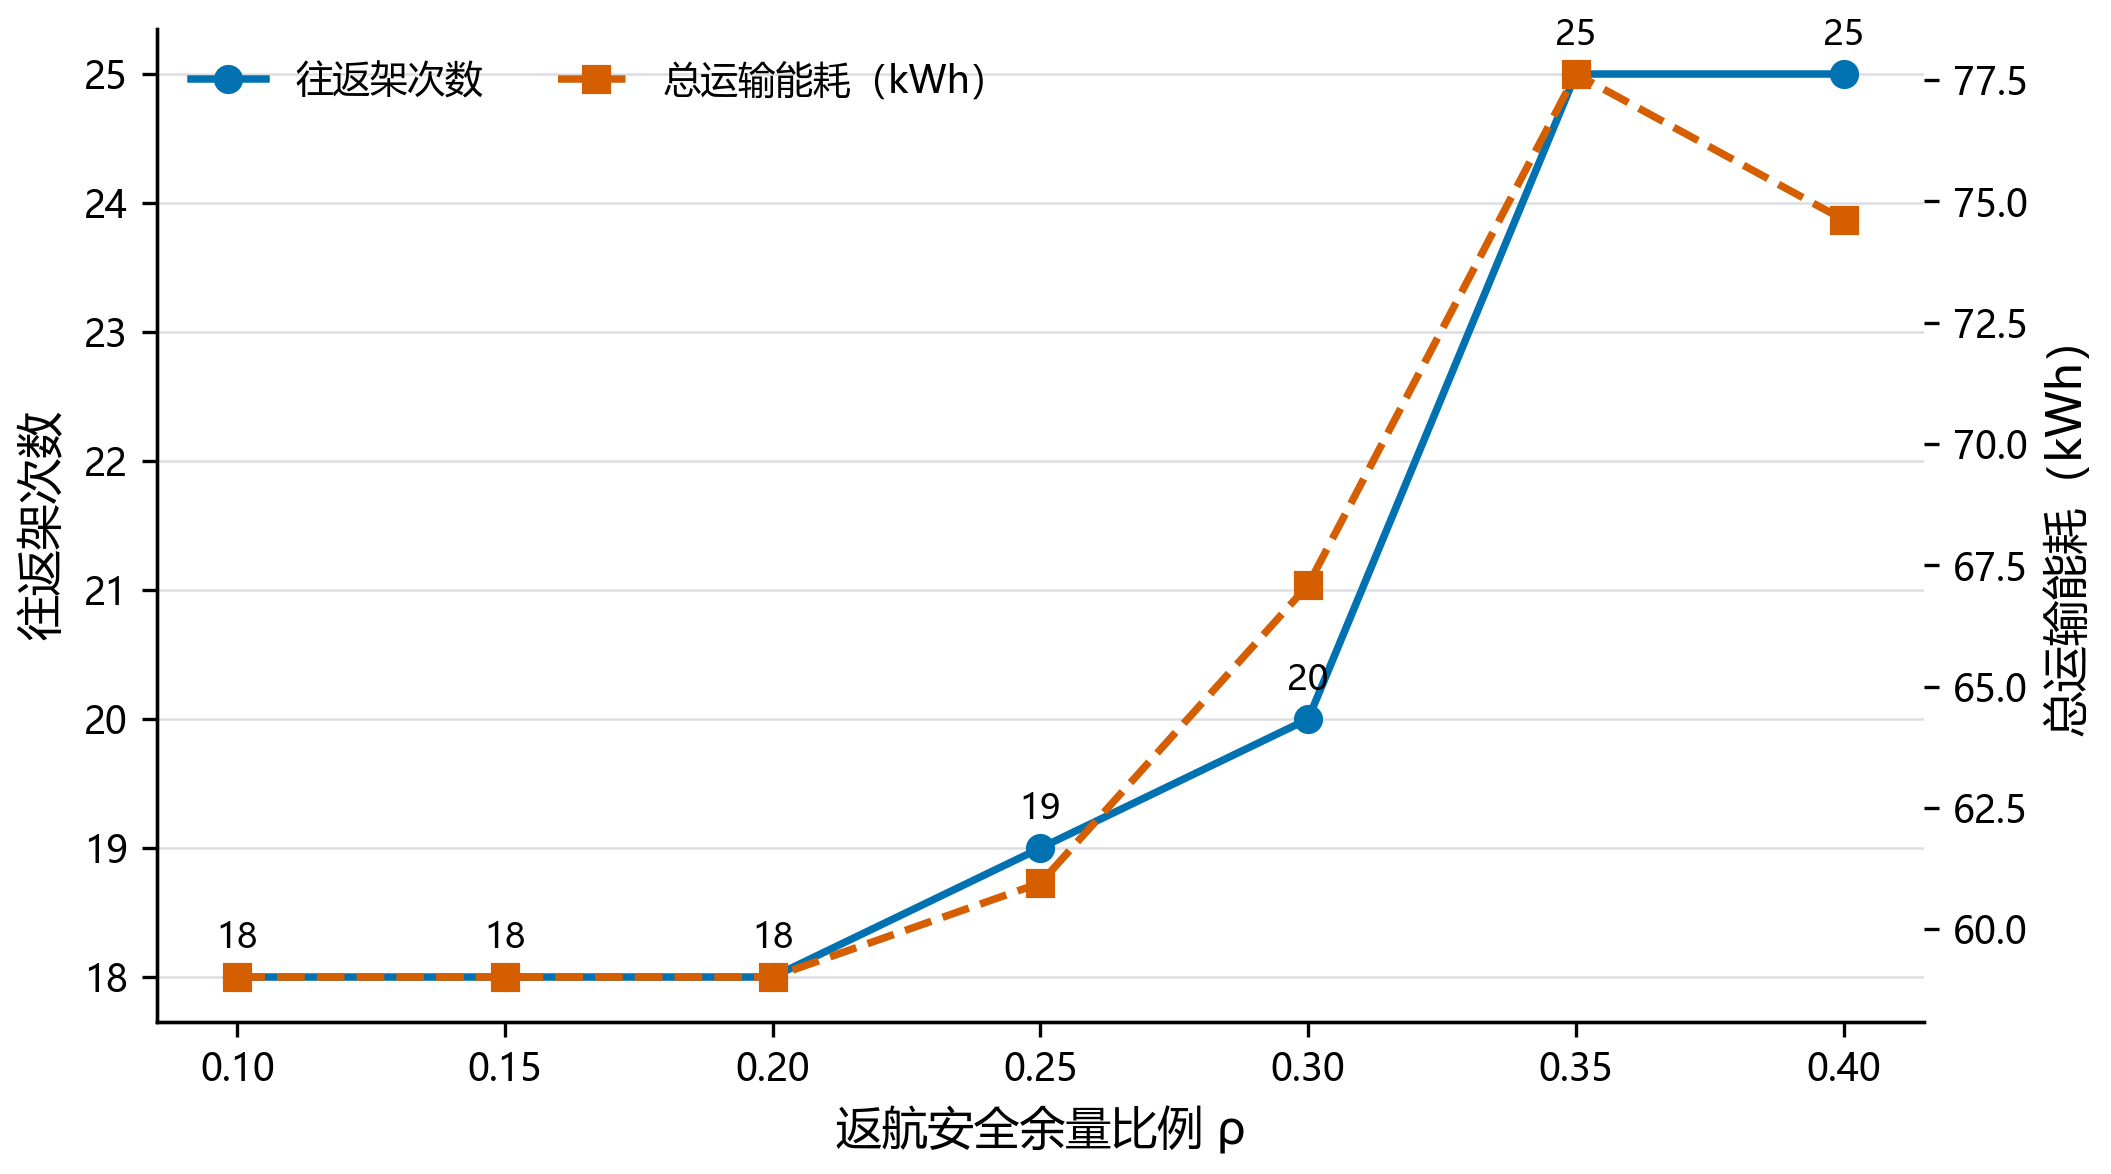
\includegraphics[width=0.74\textwidth]{figures/p1_sensitivity.png}
\caption{返航安全余量比例对架次数与总能耗的影响}
\label{fig:rho}
\end{figure}

\subsection{多目标权重的敏感性}

问题二目标函数含迟到、架次、完工、能耗四项权重。对禁忌搜索进行权重扫描，得到
7661.5\,s/73.73\,kWh、7983.2\,s/72.98\,kWh、8337.0\,s/68.06\,kWh 与
8490.3\,s/65.39\,kWh 四组零迟到方案，见表 \ref{tab:pareto}。不同权重只改变架次拆分粒度与
完工—能耗权衡，不改变重载区由 C 型承担、轻载区由 A/B 型承担的结构结论。

\subsection{中继能源预算的敏感性}

中继单架次服务时长上限由悬停转发功率决定，即 2.56\,kWh 预算除以 1.1\,kW，
约 8378\,s。本文西点连续服务 7083\,s，占上限的 84.5\%，留有约 15.5\%
余量。若未来任务量增长使时段超过上限，可将西点时段拆为两段并
在间隙返场充电，6 组能源组件支持轮换，中继方案结构不变。把悬停转发功率提高
10\%，即由 1.1\,kW 增至 1.21\,kW，上限降至约 7616\,s，仍大于 7083\,s，
方案不受影响。

\subsection{通信链路余量的敏感性}

对全部需中继采样点统计各布设点的接入链路余量，即 116\,dB 减去链路损耗，
结果如表 \ref{tab:margin} 所示，图 \ref{fig:marginhist} 给出三个布设点的余量
分布直方图。西点覆盖 1096 个采样，最紧余量 0.5\,dB，其中有 4 个采样点余量
低于 1\,dB；东点覆盖 484 个采样，最紧余量 1.0\,dB；北点覆盖 211 个采样，
最紧余量 13.4\,dB。若把接收门限提高 1\,dB，即可用余量下压 1\,dB，仅西点的
4 个采样点低于门限，只需对西点布设位置做小幅移位即可恢复全部覆盖；东点与
北点不受影响。布设方案整体对链路参数不敏感，且敏感点集中于个别低空采样，
工程上易于处理。

\begin{figure}[htbp]
\centering
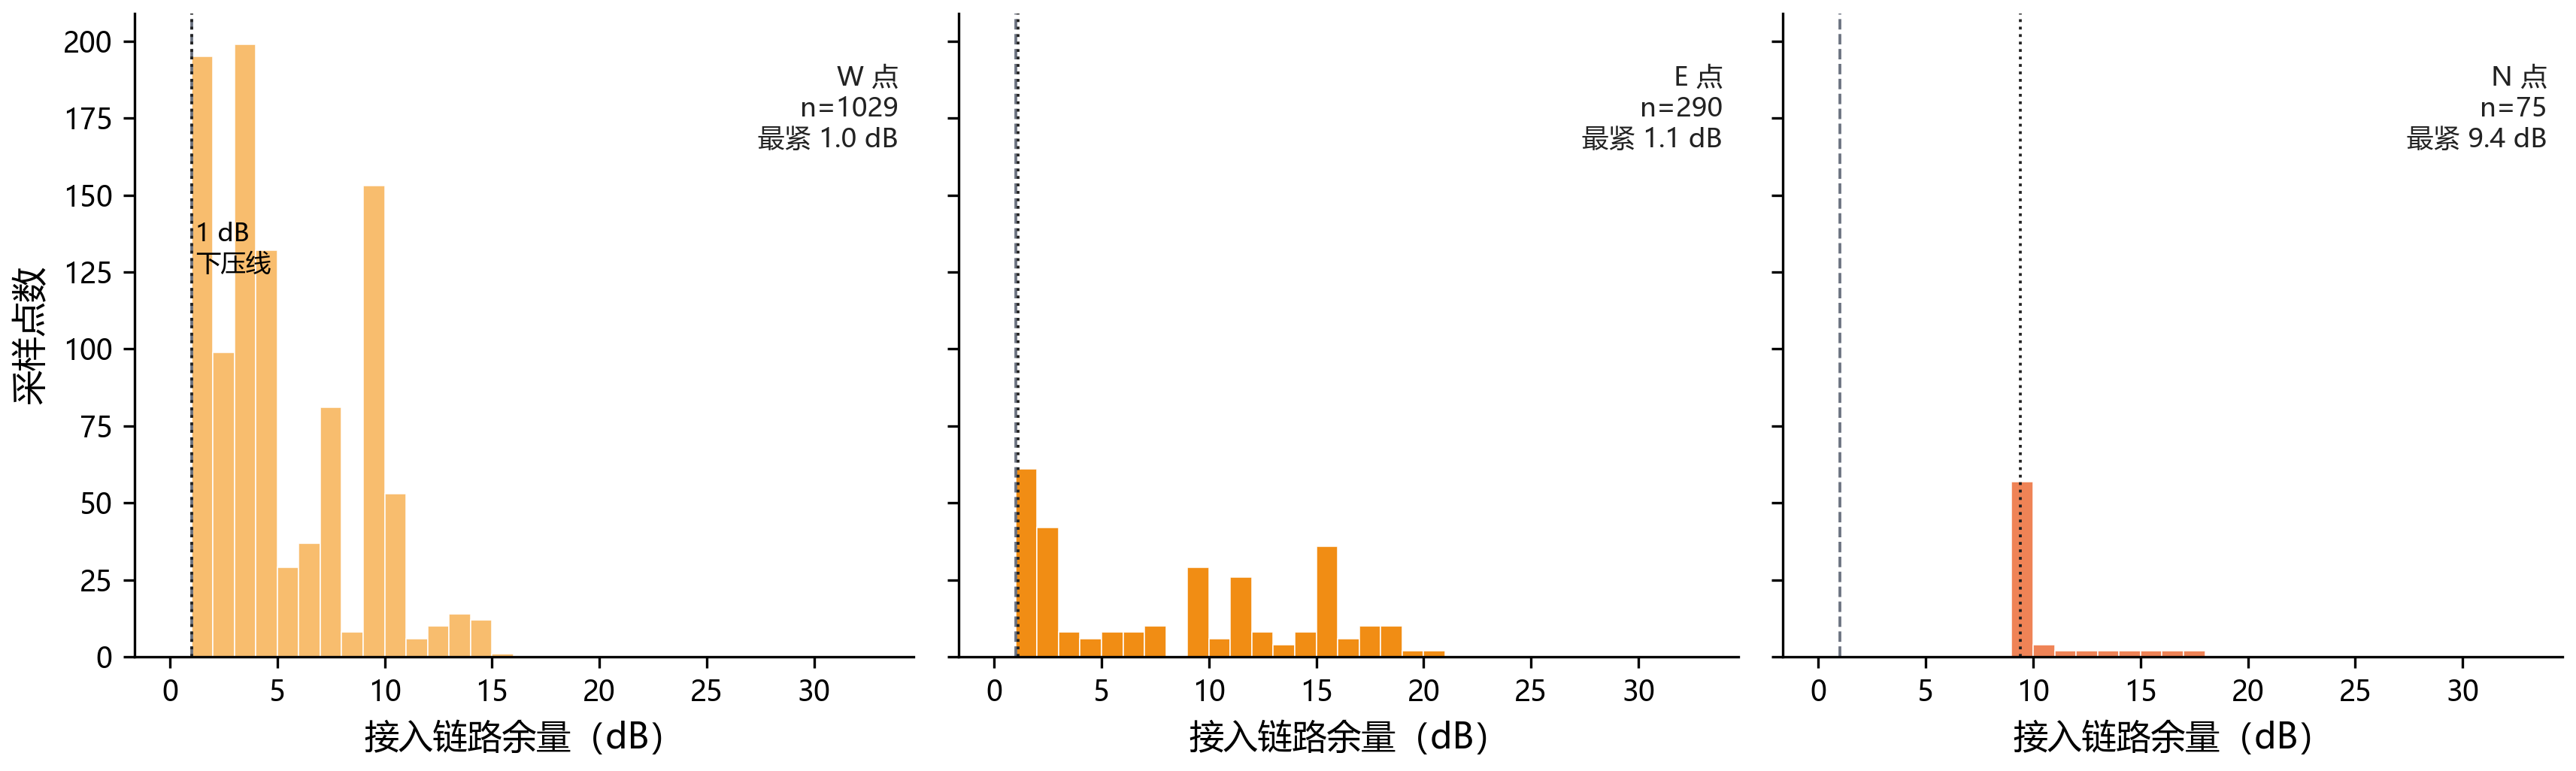
\includegraphics[width=0.98\textwidth]{figures/p3_margin_hist.png}
\caption{三个布设点接入链路余量分布（虚线为 1 dB 下压线）}
\label{fig:marginhist}
\end{figure}

\begin{table}[htbp]
\centering
\caption{各布设点接入链路余量统计（全部需中继采样点）}
\label{tab:margin}
\begin{tabular}{lcccc}
\toprule
布设点 & 覆盖采样数 & 最紧余量(dB) & 平均余量(dB) & 保障任务段数 \\
\midrule
西点 & 1096 & 0.5 & 6.2 & 33 \\
东点 & 484 & 1.0 & 13.5 & 11 \\
北点 & 211 & 13.4 & 26.0 & 4 \\
\bottomrule
\end{tabular}
\end{table}

\subsection{小结}

四类敏感性分析表明：安全余量扫描复现安全与效率的权衡且存在机型结构切换；
权重扫描确认均衡解在多目标意义下稳健；中继能源预算在 10\% 功率扰动下方案
结构不变；通信余量下压 1\,dB 时仅西点 4 个采样点接近门限，可小幅移位解决。
整体结论对参数摄动不敏感，模型可用于实际应急决策。
% 问题四
\section{问题四：任务分区与资源配置}
\label{sec:p4}

\subsection{问题分析}

问题四要求把 15 个服务区划分为两组与三组两种方案，按组配备运输无人机、电池、
中继无人机与能源组件，含冗余备份，并说明各组能否独立完成保障任务。问题四把分区与资源配置作为联合决策：分区应使各组的地理与通信需求自洽，即尽量让一组
对应一个中继布设点及其覆盖的服务区；资源配置应满足各组独立作业的时限与容量
要求，同时冗余备份需纳入库存核算。

\subsection{分区方案}

由第\ref{sec:p3}节的结论，三个中继布设点分别服务西与北片区、东片区
与 S004，且 S004 必须独立中继；第六节的 29 架次冠军全部为单区架次，
不存在跨区架次，故"同一架次涉及的服务区必须同组"的规则对分区不构成额外
约束。据此给出两种自然分区，图 \ref{fig:p4part} 以三组方案示意。

\begin{itemize}
\item 三组方案：G1 为西与北 10 区，即 S001、S002、S003、S005、S006、S007、
S008、S009、S011、S015，共 62 箱；G2 为东 4 区，即 S010、S012、
S013、S014，共 12 箱；G3 为 S004，共 6 箱。
\item 两组方案：G1 为西与北 10 区加 S004，共 11 区 68 箱；G2 为东
4 区。
\end{itemize}

\begin{figure}[htbp]
\centering
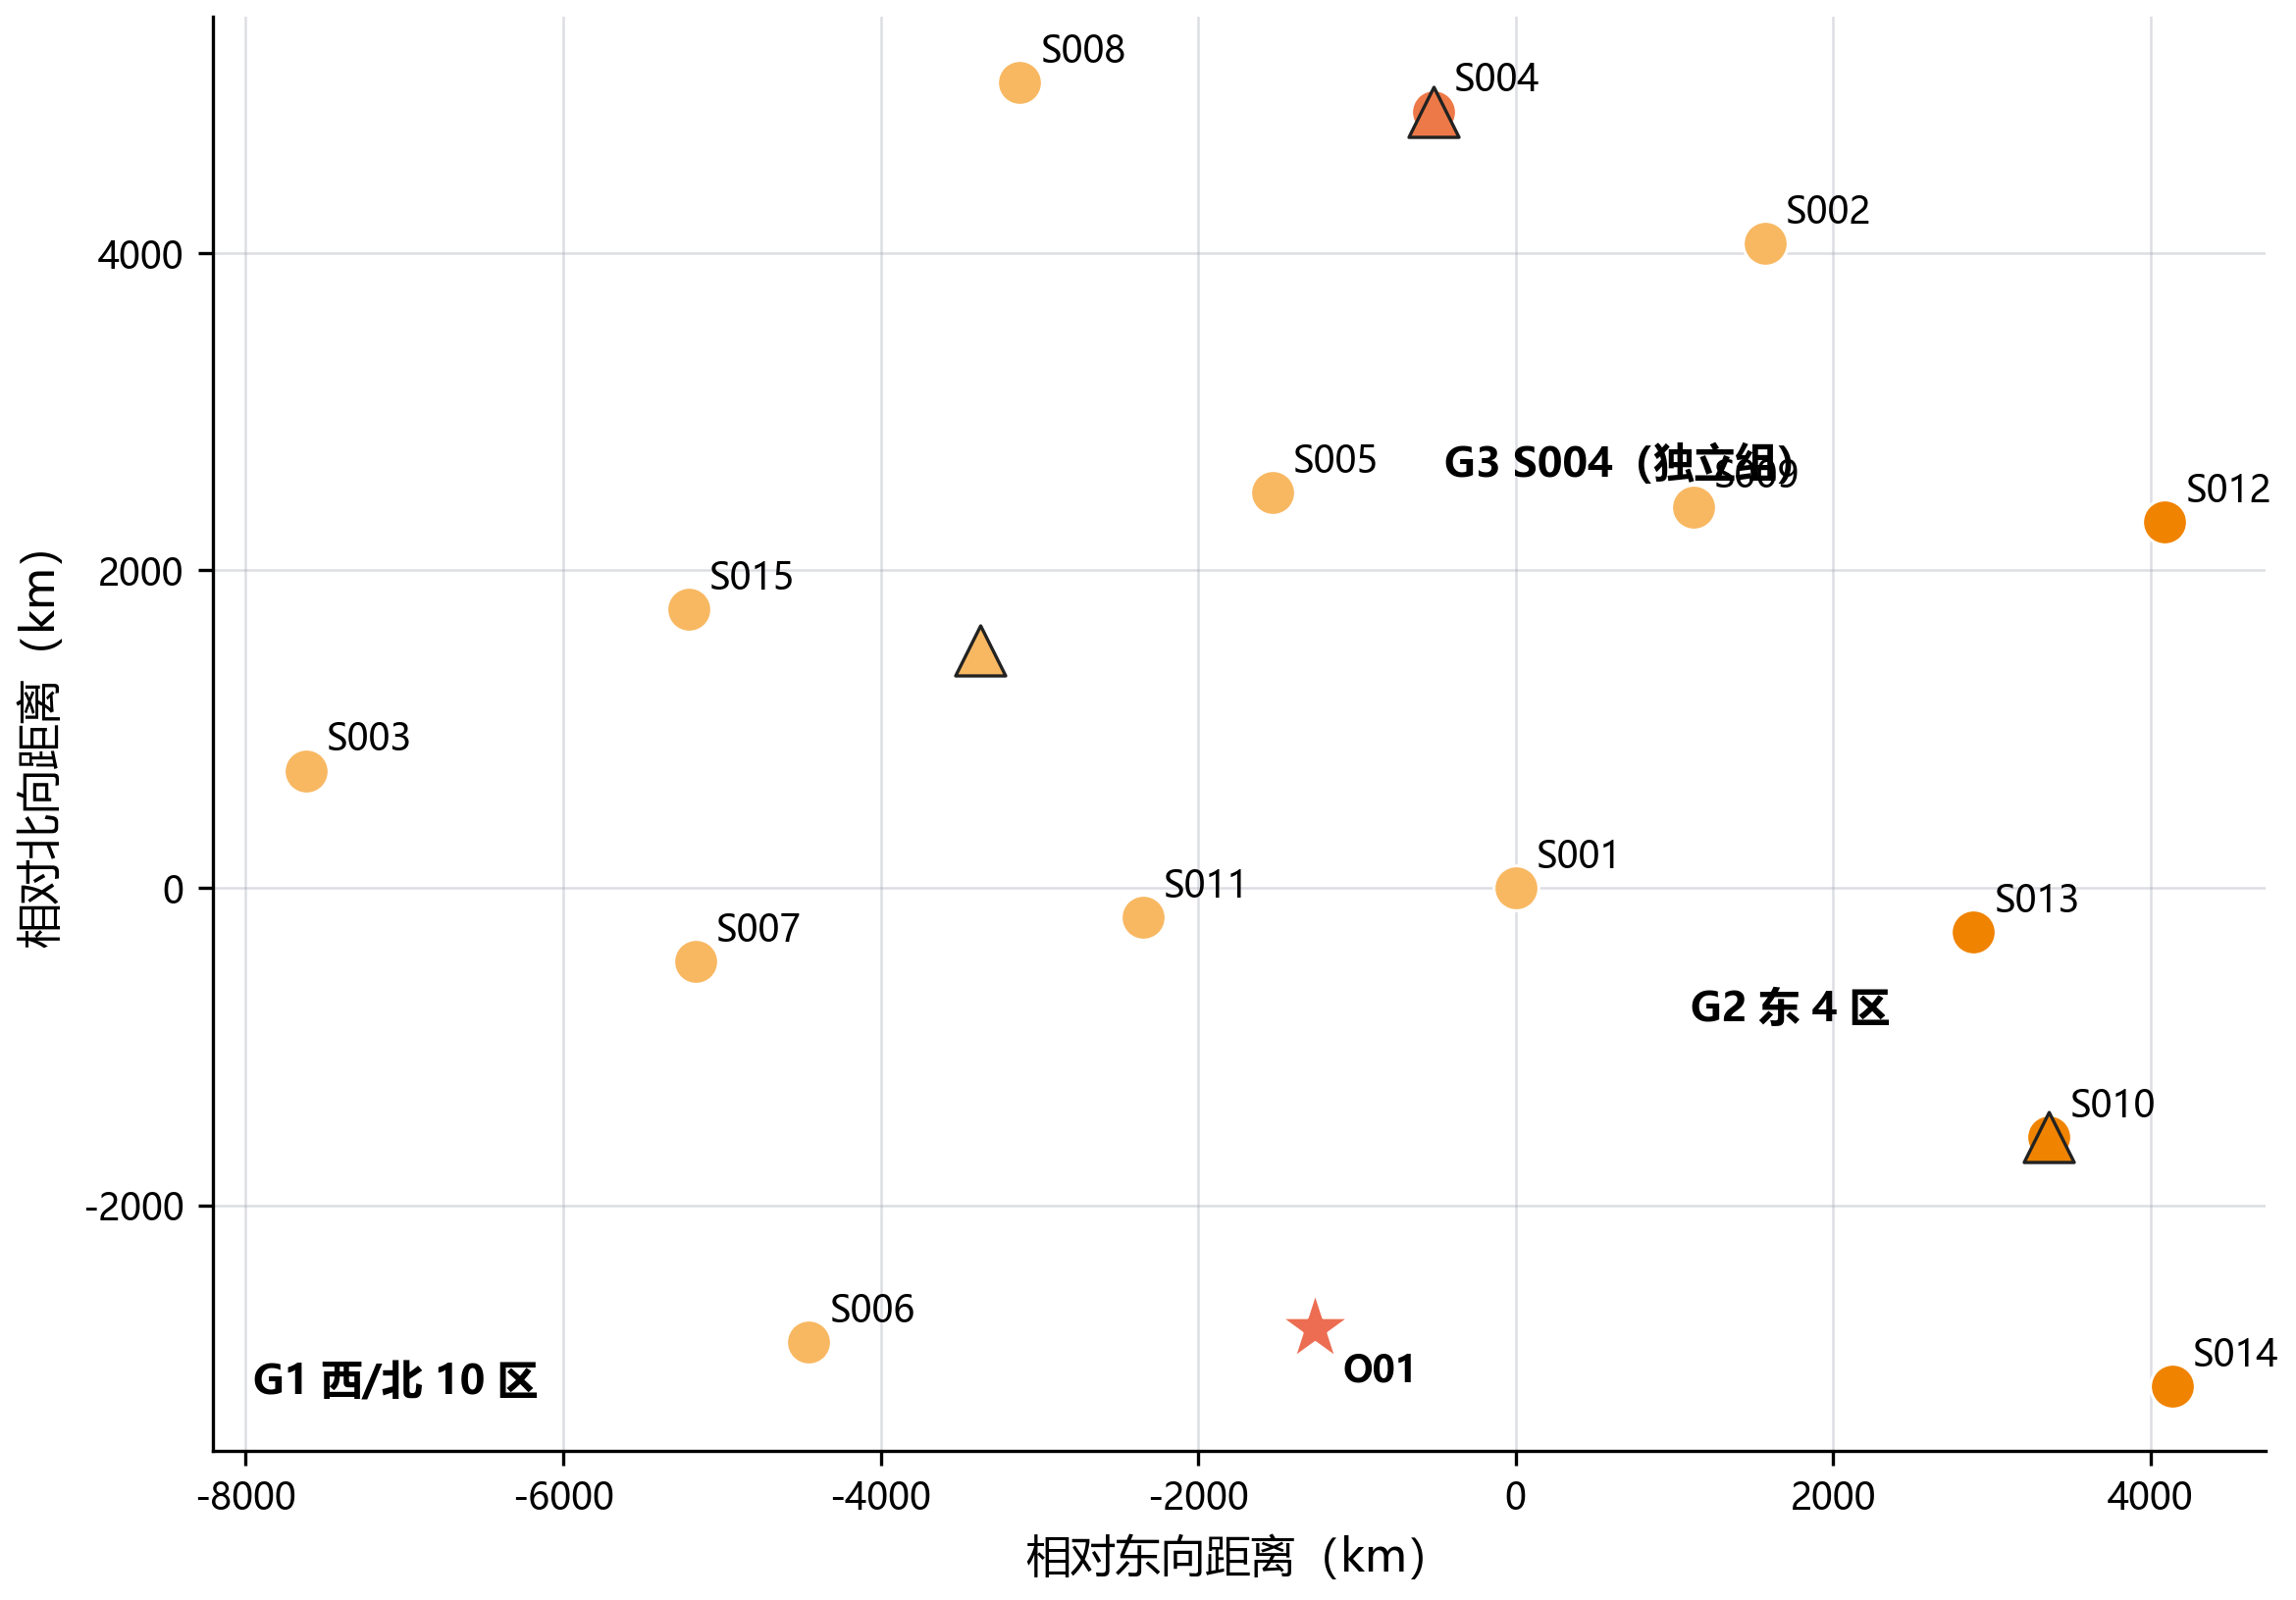
\includegraphics[width=0.76\textwidth]{figures/p4_partition.png}
\caption{三组任务分区示意（G1 西与北片区、G2 东片区、G3 为 S004）}
\label{fig:p4part}
\end{figure}

两种分区的各组负荷对比见图 \ref{fig:load}：三组方案把重载的西与北片区独立
为 G1，G2 轻载由 A/B 型自足，G3 的 S004 极小但须独享中继；两组方案把 S004
并入 G1，G1 负荷明显增大。

\begin{figure}[htbp]
\centering
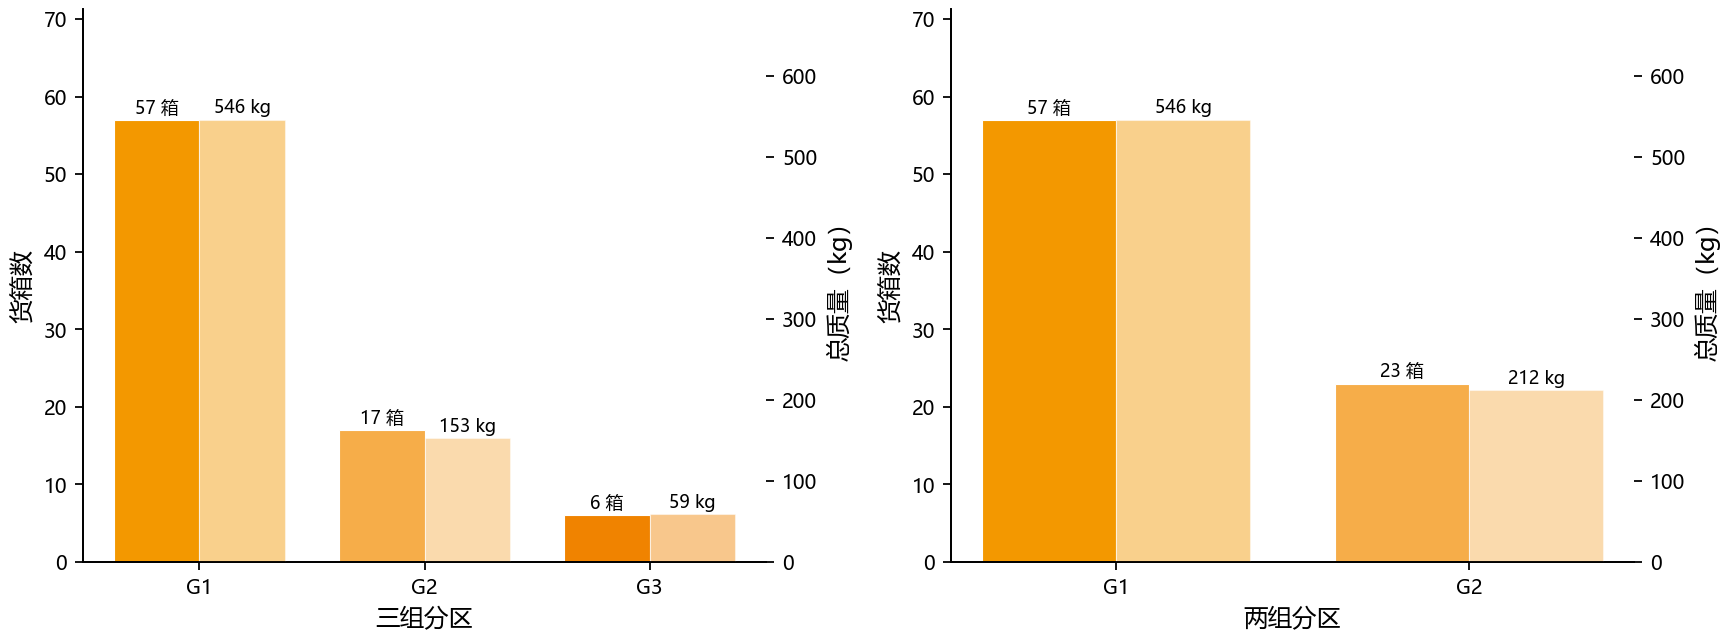
\includegraphics[width=0.98\textwidth]{figures/p4_load.png}
\caption{三组与两组方案各组货箱数与总质量对比}
\label{fig:load}
\end{figure}

\subsection{最小机队求解}

对每组执行最小机队搜索：把第六节协同方案中属于该组的货箱与架次拆出，以调度器
资源限额参数遍历机型组合与电池冗余数量，求满足全部硬时限且加权迟到为零的最小
机队。结果如表 \ref{tab:p4} 所示，各组均存在零迟到方案：三组方案下 G1（西与北
10 区）完工约 167\,min，G2（东 4 区）约 90\,min，G3（S004）约 36\,min；两组方案下
G1（西与北 10 区加 S004）完工约 155\,min，G2 约 90\,min。各组的在用机型与电池均
由 A、B、C 三类分担，其中 G1 需较多 A 型机轮转，G2 以 A/B 型自足，S004 只需
A/C 两类各 2 机。

\subsection{冗余备份与库存核算}

按在用机型加一架、电池加一组、中继加一架的方式计入冗余备份，得到各组配备
方案，见表 \ref{tab:p4}，完整明细见《结果提交模板》Q4 工作表。

\begin{table}[htbp]
\centering
\caption{分区资源配置方案（最小机队加冗余备份）}
\label{tab:p4}
\small
\begin{tabular}{llcccccccccc}
\toprule
K & 组 & 服务区 & A机 & B机 & C机 & A电 & B电 & C电 & 中继 & 组件 & 完工(s) \\
\midrule
3 & G1 & 西/北10区 & 3 & 2 & 3 & 5 & 4 & 5 & 2 & 11 & 10047 \\
3 & G2 & 东4区 & 2 & 2 & 0 & 3 & 3 & 0 & 2 & 4 & 5414 \\
3 & G3 & S004 & 2 & 0 & 2 & 2 & 0 & 2 & 3 & 2 & 2177 \\
\midrule
2 & G1 & 西/北10区+S004 & 4 & 2 & 3 & 6 & 4 & 5 & 3 & 10 & 9291 \\
2 & G2 & 东4区 & 2 & 2 & 0 & 3 & 3 & 0 & 2 & 4 & 5414 \\
\midrule
\multicolumn{3}{l}{库存} & 4 & 2 & 2 & 6 & 4 & 4 & 2 & 6 & --- \\
\bottomrule
\end{tabular}
\end{table}

\subsection{独立保障能力结论}

若坚持按组完全独立配置且含冗余，两种方案均超出给定库存。两组方案合计需
A 型机 6 架、B 型机 4 架、C 型机 3 架，分别超出库存 2、2、1 架；A 型电池 9 组、
B 型 7 组、C 型 5 组，分别超出 3、3、1 组；中继 5 架超出 3 架，能源组件 14 组
超出 8 组。三组方案分组更细导致重复配置更多，A 型机、B 型机、C 型机分别超出
3、2、3 架，A 型电池超出 4 组，中继超出 5 架，能源组件超出 11 组。缺口成因有三，
其一为西与北 G1 的 A 型任务集中，独立运转需 4 机与多组电池轮转，而轻载组也不能缺
机型保障；其二为 S004 的北点中继与各组自身中继需求并发，每组都要中继冗余；
其三为分组越细，重复配置越多，即三组方案缺口大于两组方案。

因此，在给定库存下更优的组织方式是任务分区与资源池化，即分区仅用于任务组织
与指挥协同，机队、电池与中继仍由调度中心集中调度并按时间分片复用。这正是
第六节协同方案的做法，以 8 架运输机、14 组电池、2 架中继分片服务三个时段，
恰好覆盖全部任务；零迟到与零盲区均在库存内实现。若必须完全独立按组
配置，则需增配 A 型机 2 至 3 架、B 型机 2 架、C 型机 1 至 3 架、A 型电池 3 至
4 组、B 型电池 3 组、中继 3 至 5 架与能源组件 8 至 11 组。两组与三组
方案的资源需求相对库存的缺口对比见图 \ref{fig:gap}，红色标注为超出库存的
数量，可见缺口集中在运输机与电池，且分组越细缺口越大；该结论的工程含义是：应急条件下中继等高价值资源应集中管理、按需调度；
分区用于组织指挥，不切割资源配置。

\begin{figure}[htbp]
\centering
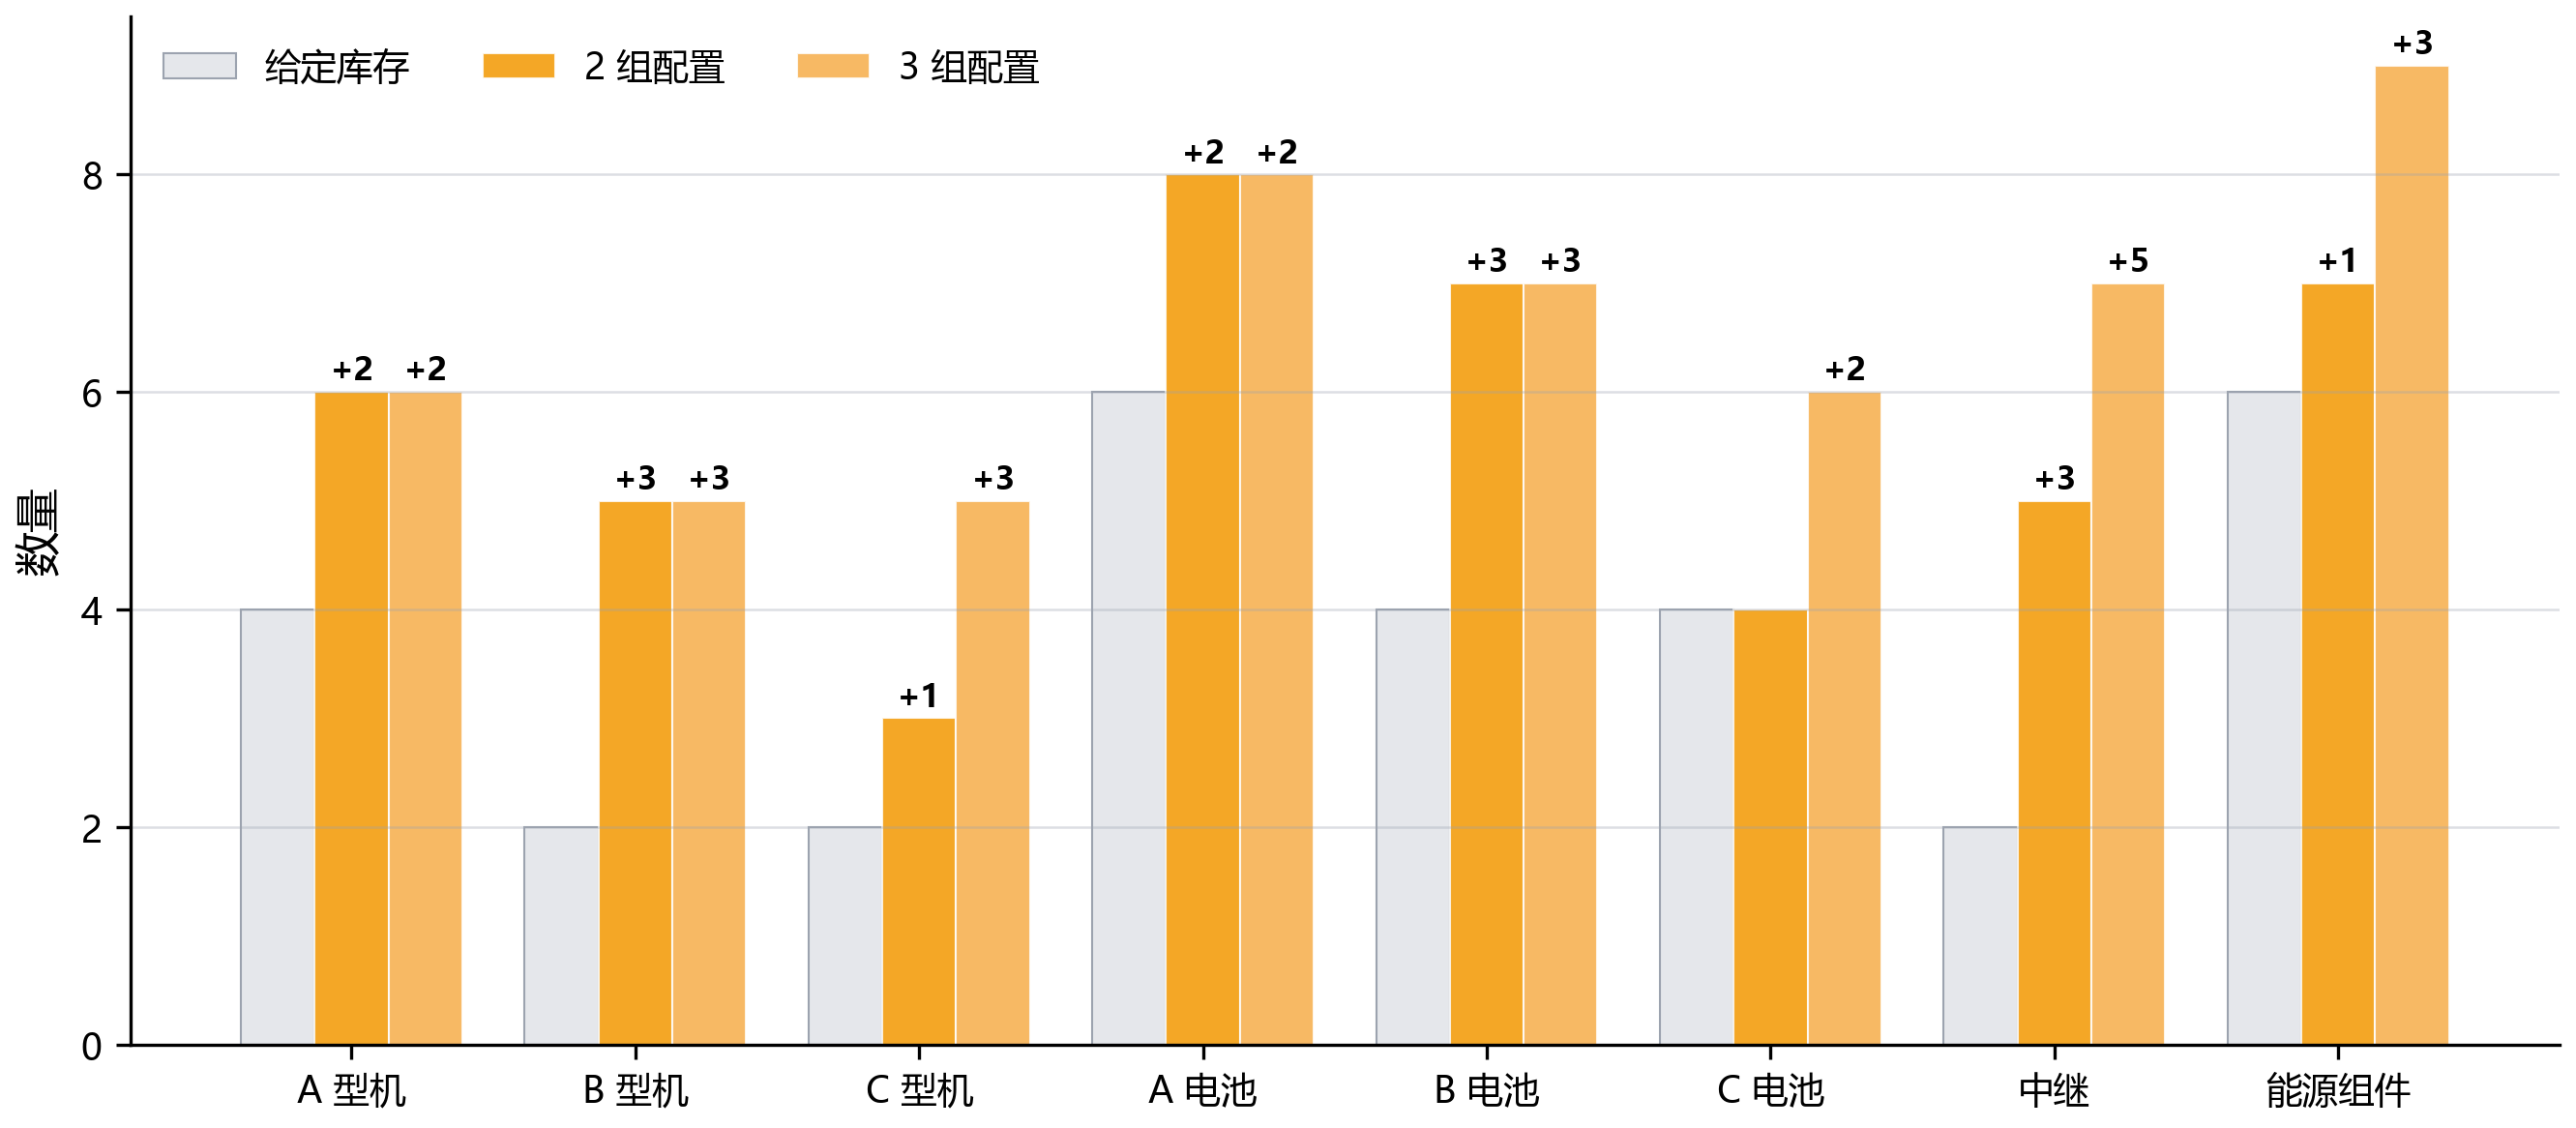
\includegraphics[width=0.96\textwidth]{figures/p4_gap.png}
\caption{两组与三组方案资源配置相对库存的缺口对比}
\label{fig:gap}
\end{figure}
% 模型评价与推广
\section{模型评价与推广}
\label{sec:eval}

\subsection{模型优点}

\begin{enumerate}
\item \textbf{物理机理一致}：能耗采用题目统一的等效航程模型，即等效航程随
载荷的 1.5 次方收缩，飞行时间按爬升、巡航、下降三段解析计算，高程取自数字
高程模型；通信按自由空间损耗加逐点地形遮挡判定，全部参数可核验，结果可复现。
\item \textbf{双层校验闭环}：运输方案以硬约束加软约束双重检验，即首飞批与
医疗货箱时限为硬约束、普通批超期加权惩罚为软约束，零迟到方案才被采纳；
通信方案以 30\,m 步长逐点采样验证，保证飞行全程无盲区是确定性判定而非估算。
\item \textbf{协同设计实现双赢}：问题三把通信窗口作为运输重排的约束而非
惩罚，通过 10 项货箱重排同时减少架次、缩短完工、降低能耗并消除盲区，体现
约束也是优化资源的建模思想。
\item \textbf{资源核算诚实}：问题四对按组独立配置与集中池化做了定量对比，
明确指出库存约束下的最优组织方式，结论具有工程可操作性。
\end{enumerate}

\subsection{模型局限}

\begin{enumerate}
\item 未考虑随机因素，即阵风、突发禁飞与设备故障，调度为确定性模型；故障
冗余仅在问题四的静态备份层面讨论。
\item 中继为单点悬停，若中继无人机遇故障，其覆盖时段将出现盲区；规模更大
时可考虑双中继并机或移动中继。
\item 电池充电按两阶段曲线近似，未建模电池老化与温度影响，荷电状态均按
线性电量核算。
\item 模拟退火的随机性使结果存在微小波动，虽以固定随机种子保证复现，但无法
保证全局最优。
\end{enumerate}

\subsection{模型推广}

\begin{enumerate}
\item \textbf{动态重规划}：将模型嵌入滚动时域框架，随灾情变化，即新需求、
道路恢复与区域失联，在线重规划，即可支持多日持续保障。
\item \textbf{多中继自组织}：把布设点集扩展为可移动中继路径，模型可推广到
中继随运输进度迁移的动态覆盖问题。
\item \textbf{异构协同场景}：模型框架，即等效航程能耗、截止期优先调度与覆盖
采样三件套，可移植到海上搜救、森林消防、重大活动保障等大范围加弱通信的
应急场景。
\end{enumerate}

% === 参考文献 ===
% 参考文献均取自题目给出的公开资料清单，与正文引用一一对应。
\begin{thebibliography}{99}
\bibitem{refXinhua} 新华社. 记者手记：抵近广西横州镇龙乡[EB/OL]. 2026-07-09[2026-08-07]. https://www.xinhuanet.com/politics/20260709/acf8e4b353304bb78007d8224f1cd2ef/c.html.
\bibitem{refXinhua2} 新华每日电讯. 三进``孤岛乡''[EB/OL]. 2026-07-12[2026-08-07]. https://www.news.cn/local/20260712/8bd1f64af3124569b5cf4415fc013acd/c.html.
\bibitem{refDEM} Copernicus Data Space Ecosystem. Copernicus DEM---Global and European Digital Elevation Model[DB/OL]. [2026-08-07]. DOI: 10.5270/ESA-c5d3d65.
\bibitem{refDorling} Dorling K, Heinrichs J, Messier G G, et al. Vehicle Routing Problems for Drone Delivery[J]. IEEE Transactions on Systems, Man, and Cybernetics: Systems, 2017, 47(1): 70-85. DOI: 10.1109/TSMC.2016.2582745.
\bibitem{refZhang} Zhang J, Campbell J F, Sweeney D C, et al. Energy Consumption Models for Delivery Drones: A Comparison and Assessment[J]. Transportation Research Part D: Transport and Environment, 2021, 90: 102668. DOI: 10.1016/j.trd.2020.102668.
\bibitem{refITU} International Telecommunication Union. Recommendation ITU-R P.525-5: Calculation of Free-Space Attenuation[S/OL]. 2024. https://www.itu.int/rec/R-REC-P.525-5-202411-I/en.
\bibitem{refTI} Texas Instruments. Li-Ion Battery Charger Solution Using an MSP430 MCU[EB/OL]. https://www.ti.com/lit/an/slaa287b/slaa287b.pdf.
\bibitem{refZeng} Zeng Y, Zhang R, Lim T J. Wireless Communications with Unmanned Aerial Vehicles: Opportunities and Challenges[J]. IEEE Communications Magazine, 2016, 54(5): 36-42. DOI: 10.1109/MCOM.2016.7470933.
\bibitem{refDJI} DJI Enterprise. Matrice 350 RTK Specifications[EB/OL]. https://enterprise.dji.com/matrice-350-rtk/specs.
\bibitem{refDoodle} Doodle Labs. Sense: Interference Avoidance[EB/OL]. https://doodlelabs.com/news/sense-interference-avoidance-release/.
\end{thebibliography}

% === 附录 ===
\begin{appendices}
\section{核心代码}

本节给出可复现全文关键结果的核心程序（节选）。完整可运行代码、数据与全部结果
文件随附件一并交付（\texttt{solve\_d/code/} 目录），核心脚本分工如下：
\begin{itemize}
    \item \texttt{core.py}：数据装载、DEM 读取、航线几何（巡航高度/三段时间）、
    等效航程能耗、两阶段充电、链路损耗与遮挡判定、中继转场时间/能耗；
    \item \texttt{p1\_solve.py}：问题一最大安全载荷二分求解与货箱组批；
    \item \texttt{p2\_solve.py}：问题二模拟退火调度器（截止期优先派单与资源限额）；
    \item \texttt{p3\_construct.py}：问题三货箱重排与中继时序构造（最终方案）；
    \item \texttt{p3\_margins.py}：问题三各中继布设点链路余量统计重算；
    \item \texttt{p3\_figures.py}、\texttt{p2\_figures.py}：论文图件；
    \item \texttt{p4\_solve.py}：问题四最小机队搜索与分区核算；
    \item \texttt{export\_excel.py}：写入《结果提交模板.xlsx》六个工作表。
\end{itemize}
运行环境：Python 3.14 + numpy/scipy/pandas/openpyxl/matplotlib。

本论文的数据分析、模型构建与写作在人工智能工具辅助下完成。工具名称：DSH
(glm-5.3)；开发机构：智谱AI；版本发布日期：2026-04。所有数值结果均由随附脚本在
题目原始数据上复算获得，可在本机直接重跑验证。

\begin{Python}{等效航程能耗与安全约束（core.py 节选）}
# 本程序及代码是在人工智能工具辅助下完成的。
# 工具名称：DSH (glm-5.3)；开发机构：智谱AI；发布日期：2026-04。
import numpy as np

RHO = 0.2                      # 返航安全裕度
G = 9.81

def flight_profile(nodes, loads, g, data):
    """nodes: [(lon,lat)]；loads: 各航段载荷。返回 (t_fly, E_total)。"""
    p = data.uav_types[g]
    t = 0.0
    e = 0.0
    z0 = data.gw_pt['z']       # O01 地面高程
    for i in range(len(nodes) - 1):
        lon1, lat1 = nodes[i]; lon2, lat2 = nodes[i + 1]
        # 巡航高度 = 航段 DEM 最高点 + 50m
        d, cruise, h_up, h_down = segment_geometry(lon1, lat1, lon2, lat2, data)
        q = loads[i]
        # 三段时间
        t += h_up / p['v_up'] + d / p['v_c'] + h_down / p['v_down']
        # 水平能耗（等效航程折算）
        Lg = p['L0'] - (p['L0'] - p['LF']) * (q / p['Q']) ** 1.5
        e += p['E_use'] * d / Lg
        # 爬升能耗
        e += (p['m0'] + q) * G * h_up / (p['eta'] * 3.6e6)
    return t, e

def feasible(q, nodes, loads, g, data):
    _, e = flight_profile(nodes, loads, g, data)
    return e <= (1 - RHO) * data.uav_types[g]['E_use']
\end{Python}

\begin{Python}{EDF 派单与资源就绪队列（p2\_solve.py 节选）}
def dispatch(data, flights, releases=None, limit=None):
    """EDF 排序 + 无人机/电池就绪队列；limit 支持问题四最小机队搜索。"""
    if releases is None:
        releases = {}
    if limit is None:
        limit = {'A': (4, 6), 'B': (2, 4), 'C': (2, 4)}
    uavs = {}                  # uid -> (ready_time, battery)
    batteries = {}             # bid -> ready_time
    schedule = {}
    for f in sorted(flights, key=critical_time):
        model = f.model
        n_uav, n_bat = limit[model]
        cand = [u for u, st in uavs.items() if st[0] <= t_now and model_of(u) == model]
        # 最早可用的无人机 + 满电电池
        u = min(cand, key=lambda u: uavs[u][0])
        b = min(batteries, key=lambda b: batteries[b])
        t_start = max(releases.get(f.fid, 0.0), uavs[u][0], batteries[b]) + prep(f)
        t_ret = t_start + f.time()
        schedule[f.fid] = {'uav': u, 'battery': b, 'start': t_start,
                           'return': t_ret, 'energy': f.energy()}
        uavs[u] = (t_ret, b)
        batteries[b] = t_ret + charge_time(1 - f.energy() / E_use(model))
    return schedule, uavs
\end{Python}

\begin{Python}{通信链路判定（core.py 节选）}
def path_loss(lon1, lat1, z1, lon2, lat2, z2, data):
    d3 = np.sqrt(dist_2d(lon1, lat1, lon2, lat2) ** 2 + (z1 - z2) ** 2 / 1e3 ** 2)
    L = 32.45 + 20 * np.log10(2400) + 20 * np.log10(d3 * 1e3)  # d3: km
    if los_occluded(lon1, lat1, z1, lon2, lat2, z2, data):
        L += 10.0
    return L

def los_occluded(lon1, lat1, z1, lon2, lat2, z2, data):
    """沿连线 30m 步长采样 DEM，任一点地形高于连线即遮挡。"""
    n = max(2, int(dist_2d(lon1, lat1, lon2, lat2) / 0.03))
    for k in range(1, n):
        f = k / n
        lon = lon1 + (lon2 - lon1) * f
        lat = lat1 + (lat2 - lat1) * f
        zline = z1 + (z2 - z1) * f
        if data.dem_at(lon, lat) > zline:
            return True
    return False

def direct_ok(lon, lat, z, data):
    L = path_loss(lon, lat, z, data.gw_pt['lon'], data.gw_pt['lat'], z + 50, data)
    return L <= 122.0            # 直连链路上限 122 dB
\end{Python}
\end{appendices}

\end{document} 
